\documentclass[11pt,fleqn]{book}
\usepackage[top=3cm,bottom=3cm,left=3.2cm,right=3.2cm,headsep=10pt,letterpaper]{geometry}
%中文支持
\usepackage[space]{ctex}
\usepackage{amsmath}
\usepackage{amssymb}
\usepackage{times}
\usepackage{titlesec}
%结构化
\graphicspath{{./pic/chapter1/}{./pic/chapter2/}{./pic/chapter3/}}
\usepackage{subfiles}
\usepackage{blindtext}
\usepackage{listings}%设置C风格代码格式
\usepackage{graphicx}
\usepackage{float}
\usepackage{pythonhighlight}
\usepackage{caption}
\usepackage{subfigure}
\usepackage{longtable}
\setlength{\arrayrulewidth}{1mm}
\usepackage{hyperref}
\usepackage{amsmath}
\pagenumbering{arabic}
\hypersetup{
    colorlinks=true,
    linkcolor=blue,
    filecolor=magenta,      
    urlcolor=cyan,
}
\urlstyle{same}
%字体设置
\usepackage{avant} % Use the Avantgarde font for headings
%\usepackage{times} % Use the Times font for headings
\usepackage{mathptmx} % Use the Adobe Times Roman as the default text font together with math symbols from the Sym­bol, Chancery and 
%tktz画图
\usepackage{tkz-graph}
\GraphInit[vstyle = Shade]
\tikzset{
  LabelStyle/.style = { rectangle, rounded corners, draw,
                        minimum width = 2em, fill = green!50,
                        text = red, font = \bfseries },
  VertexStyle/.append style = { inner sep=5pt,
                                font = \Large\bfseries},
  EdgeStyle/.append style = {->, bend left} }

\begin{document}
\frontmatter
\tableofcontents % Print the table of contents itself
\mainmatter
\lstset{numbers=left,numberstyle=\tiny,keywordstyle=\color{blue!70}, commentstyle=\color{red!50!green!50!blue!50},frame=shadowbox,rulesepcolor=\color{red!20!green!20!blue!20},escapeinside=``}
\chapter{deeplearning}
\section{降维}
\subsection{自编码}
人工神经网络(ANN)本身就是具有层次结构的系统,如果给定一个神经网络,我们假设其输出与输入是相同的,然后训练调整其参数,得到每一层中的权重。自然地,我们就得到了输入I的几种不同表示(每一层代表一种表示),这些表示就是特征。在研究中可以发现,如果在原有的特征中加入这些自动学习得到的特征可以大大提高精确度,甚至在分类问题中比目前最好的分类算法效果还要好!这种方法称为AutoEncoder(自动编码器)。自动编码器就是一种尽可能复现输入信号的神经网络。为了实现这种复现,自动编码器就必须捕捉可以代表输入数据的最重要的因素,就像PCA那样,找到可以代表原信息的主要成分。
我们将input输入一个encoder编码器,就会得到一个code,这个code也就是输入的一个表示,那么我们怎么知道这个code表示的就是input呢?我们加一个decoder解码器,这时候decoder就会输出一个信息,那么如果输出的这个信息和一开始的输入信号input是很像的(理想情况下就是一样的),那很明显,我们就有理由相信这个code是靠谱的。所以,我们就通过调整encoder和decoder的参数,使得重构误差最小,这时候我们就得到了输入input信号的第一个表示了,也就是编码code了。因为是无标签数据,所以误差的来源就是直接重构后与原输入相比得到。
\subsection{自动降噪编码}
以一定的概率分布擦出原始数据(将数据置为0),这样操作后的数据称为破损数据,这样的数据有两个作用:
\begin{enumerate}
\item 通过破损数据和非破损数据相比,破损数据训练出来的权重噪声小(可能不小心删除了噪声)。
\item 破损数据一定程度上减轻了训练数据和测试数据之间的代沟。由于数据部分被擦除,因而训练出来的权重的健壮性就提高了。
\end{enumerate}
\subsection{手写体数据自编码}
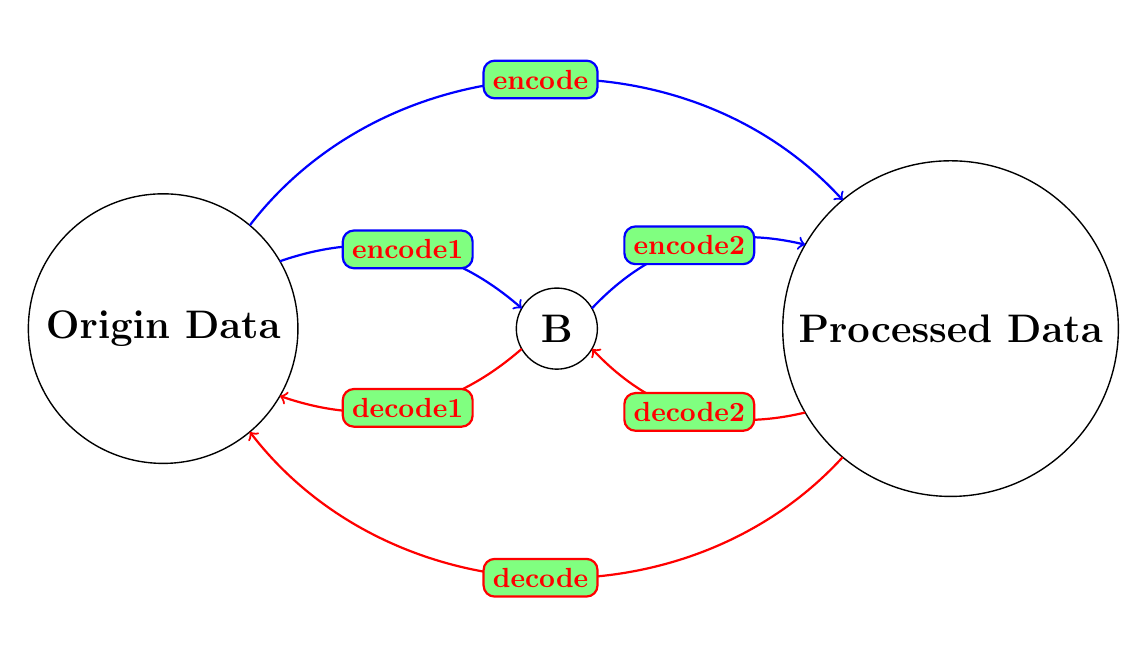
\begin{tikzpicture}
  \SetGraphUnit{5}
  \Vertex{B}
  \WE(B){Origin Data}
  \EA(B){Processed Data}
  \Edge[label = encode1,color = blue](Origin Data)(B)
  \Edge[label = encode2,color = blue](B)(Processed Data)
  \Edge[label = decode2,color = red](Processed Data)(B)
  \Edge[label = decode1,color = red](B)(Origin Data)
  \tikzset{EdgeStyle/.append style = {bend left = 50}}
  \Edge[label = encode,color=blue](Origin Data)(Processed Data)
  \Edge[label = decode,color=red](Processed Data)(Origin Data)
\end{tikzpicture}

\begin{python}
import tensorflow as tf
import matplotlib.pyplot as plt
data_path = '/home/hpc/文档/mnist_tutorial/mnist'

from tensorflow.examples.tutorials.mnist import input_data
mnist = input_data.read_data_sets(data_path, one_hot=False)


# Visualize decoder setting
learning_rate = 0.01
training_epochs = 5
batch_size = 256
display_step = 1
examples_to_show = 10

n_input = 784  # MNIST data input (img shape: 28*28)

x = tf.placeholder(tf.float32,[None,n_input])

n_hidden_1 = 256
n_hidden_2 = 128
weights = {
    'encode_h1':tf.Variable(tf.random_normal([n_input,n_hidden_1])),
    'encode_h2':tf.Variable(tf.random_normal([n_hidden_1,n_hidden_2])),
    'decode_h2':tf.Variable(tf.random_normal([n_hidden_2,n_hidden_1])),
    'decode_h1':tf.Variable(tf.random_normal([n_hidden_1,n_input]))
}
bias = {'encode_h1':tf.Variable(tf.random_normal([n_hidden_1])),
    'encode_h2':tf.Variable(tf.random_normal([n_hidden_2])),
    'decode_h2':tf.Variable(tf.random_normal([n_hidden_1])),
    'decode_h1':tf.Variable(tf.random_normal([n_input]))

}
def encode(x):
    layer_1 = tf.nn.sigmoid(tf.add(tf.matmul(x,weights['encode_h1']),bias['encode_h1']))
    layer_2 = tf.nn.sigmoid(tf.add(tf.matmul(layer_1,weights['encode_h2']),bias['encode_h2']))
    return layer_2

def decode(x):
    layer_1 = tf.nn.sigmoid(tf.add(tf.matmul(x,weights['decode_h2']),bias['decode_h2']))
    layer_2 = tf.nn.sigmoid(tf.add(tf.matmul(layer_1,weights['decode_h1']),bias['decode_h1']))
    return layer_2



encode_op = encode(x)
decode_op = decode(encode_op)
y_pred = decode_op
y_true = x
cost = tf.reduce_mean(tf.square(y_pred-y_true))
optimizer = tf.train.AdamOptimizer(learning_rate).minimize(cost)

with tf.Session() as sess:
    init = tf.global_variables_initializer()
    sess.run(init)
    total_batch = int(mnist.train.num_examples/batch_size)
    for epoch in range(training_epochs):
        for i in range(total_batch):
            batch_xs,batch_ys = mnist.train.next_batch(batch_size)
            _, c = sess.run([optimizer, cost], feed_dict={x: batch_xs})
        if epoch%display_step==0:
            print("Epoch:",'%04d'%(epoch+1),'cost=','{:.9f}'.format(c))
    print('Optimize finish')
    encode_decode = sess.run(y_pred,feed_dict={x:mnist.test.images[:examples_to_show]})
    f,a = plt.subplots(2,10,figsize=(10,2))
    for i in range(examples_to_show):
        a[0][i].imshow(sess.run(tf.reshape(mnist.test.images[i],[28,28])))
        a[1][i].imshow(sess.run(tf.reshape(encode_decode[i],[28,28])))
    plt.savefig('auto_encode.png',dpi=800)
\end{python}
\begin{center}
\begin{figure}[H]
\includegraphics[scale=0.5]{auto_encode.png}
\caption{原图和自编码解码后的图像}
\end{figure}
\end{center}
编码器输出可视化:
\begin{python}
import tensorflow as tf
import matplotlib.pyplot as plt

from tensorflow.examples.tutorials.mnist import input_data
path = '/home/hpc/文档/mnist_tutorial/mnist'
mnist = input_data.read_data_sets(path, one_hot=False)

learning_rate = 0.01
training_epochs = 5
batch_size = 256
display_step = 1
examples_to_show = 10

n_input = 784  # MNIST data input (img shape: 28*28)

X = tf.placeholder("float", [None, n_input])

n_hidden_1 = 256 # 1st layer num features
n_hidden_2 = 128 # 2nd layer num features

learning_rate = 0.01    # 0.01 this learning rate will be better! Tested
training_epochs = 10
batch_size = 256
display_step = 1
n_input = 784  # MNIST data input (img shape: 28*28)
X = tf.placeholder("float", [None, n_input])
n_hidden_1 = 128
n_hidden_2 = 64
n_hidden_3 = 10
n_hidden_4 = 2
weights = {
    'encoder_h1': tf.Variable(tf.truncated_normal([n_input, n_hidden_1],)),
    'encoder_h2': tf.Variable(tf.truncated_normal([n_hidden_1, n_hidden_2],)),
    'encoder_h3': tf.Variable(tf.truncated_normal([n_hidden_2, n_hidden_3],)),
    'encoder_h4': tf.Variable(tf.truncated_normal([n_hidden_3, n_hidden_4],)),
    'decoder_h1': tf.Variable(tf.truncated_normal([n_hidden_4, n_hidden_3],)),
    'decoder_h2': tf.Variable(tf.truncated_normal([n_hidden_3, n_hidden_2],)),
    'decoder_h3': tf.Variable(tf.truncated_normal([n_hidden_2, n_hidden_1],)),
    'decoder_h4': tf.Variable(tf.truncated_normal([n_hidden_1, n_input],)),
}
biases = {
    'encoder_b1': tf.Variable(tf.random_normal([n_hidden_1])),
    'encoder_b2': tf.Variable(tf.random_normal([n_hidden_2])),
    'encoder_b3': tf.Variable(tf.random_normal([n_hidden_3])),
    'encoder_b4': tf.Variable(tf.random_normal([n_hidden_4])),
    'decoder_b1': tf.Variable(tf.random_normal([n_hidden_3])),
    'decoder_b2': tf.Variable(tf.random_normal([n_hidden_2])),
    'decoder_b3': tf.Variable(tf.random_normal([n_hidden_1])),
    'decoder_b4': tf.Variable(tf.random_normal([n_input])),
}
def encoder(x):
    layer_1 = tf.nn.sigmoid(tf.add(tf.matmul(x, weights['encoder_h1']),
                                   biases['encoder_b1']))
    layer_2 = tf.nn.sigmoid(tf.add(tf.matmul(layer_1, weights['encoder_h2']),
                                   biases['encoder_b2']))
    layer_3 = tf.nn.sigmoid(tf.add(tf.matmul(layer_2, weights['encoder_h3']),
                                   biases['encoder_b3']))
    layer_4 = tf.add(tf.matmul(layer_3, weights['encoder_h4']),
                                    biases['encoder_b4'])
    return layer_4
def decoder(x):
    layer_1 = tf.nn.sigmoid(tf.add(tf.matmul(x, weights['decoder_h1']),
                                   biases['decoder_b1']))
    layer_2 = tf.nn.sigmoid(tf.add(tf.matmul(layer_1, weights['decoder_h2']),
                                   biases['decoder_b2']))
    layer_3 = tf.nn.sigmoid(tf.add(tf.matmul(layer_2, weights['decoder_h3']),
                                biases['decoder_b3']))
    layer_4 = tf.nn.sigmoid(tf.add(tf.matmul(layer_3, weights['decoder_h4']),
                                biases['decoder_b4']))
    return layer_4

encoder_op = encoder(X)
decoder_op = decoder(encoder_op)

y_pred = decoder_op
y_true = X

cost = tf.reduce_mean(tf.pow(y_true - y_pred, 2))
optimizer = tf.train.AdamOptimizer(learning_rate).minimize(cost)


with tf.Session() as sess:
    init = tf.global_variables_initializer()
    sess.run(init)
    total_batch = int(mnist.train.num_examples/batch_size)
    for epoch in range(training_epochs):
        for i in range(total_batch):
            batch_xs, batch_ys = mnist.train.next_batch(batch_size)  # max(x) = 1, min(x) = 0
            _, c = sess.run([optimizer, cost], feed_dict={X: batch_xs})
        if epoch % display_step == 0:
            print("Epoch:", '%04d' % (epoch+1),
                  "cost=", "{:.9f}".format(c))
    print("Optimization Finished!")
    encode_decode = sess.run(
        y_pred, feed_dict={X: mnist.test.images[:examples_to_show]})
    encoder_result = sess.run(encoder_op, feed_dict={X: mnist.test.images})
    plt.scatter(encoder_result[:, 0], encoder_result[:, 1], c=mnist.test.labels)
    plt.title('encode output')
    plt.colorbar()
    plt.savefig('auto_encode_v.png',dpi=800)
\end{python}

\begin{center}
\begin{figure}[H]
\includegraphics[scale=0.7]{auto_encode_v.png}
\end{figure}
\end{center}
\section{稀疏编码}
稀疏编码算法是一种无监督学习方法,它用来寻找一组“超完备”基向量来更高效地表示样本数据。稀疏编码算法的目的就是找到一组基向量 $\mathbf{\phi}_i$ ,使得我们能将输入向量 $\mathbf{x}$ 表示为这些基向量的线性组合:
\begin{align}
\mathbf{x} = \sum_{i=1}^k a_i \mathbf{\phi}_{i} 
\end{align}
虽然形如主成分分析技术(PCA)能使我们方便地找到一组“完备”基向量,但是这里我们想要做的是找到一组“超完备”基向量来表示输入向量 $\mathbf{x}\in\mathbb{R}^n$ (也就是说,k > n)。超完备基的好处是它们能更有效地找出隐含在输入数据内部的结构与模式。然而,对于超完备基来说,系数$a_i$不再由输入向量 $\mathbf{x}$ 唯一确定。因此,在稀疏编码算法中,我们另加了一个评判标准“稀疏性”来解决因超完备而导致的退化(degeneracy)问题。

这里,我们把“稀疏性”定义为:只有很少的几个非零元素或只有很少的几个远大于零的元素。要求系数$a_i$ 是稀疏的意思就是说:对于一组输入向量,我们只想有尽可能少的几个系数远大于零。选择使用具有稀疏性的分量来表示我们的输入数据是有原因的,因为绝大多数的感官数据,比如自然图像,可以被表示成少量基本元素的叠加,在图像中这些基本元素可以是面或者线。同时,比如与初级视觉皮层的类比过程也因此得到了提升。

我们把有 m 个输入向量的稀疏编码代价函数定义为:
\begin{align}
\text{minimize}_{a^{(j)}_i,\mathbf{\phi}_{i}} \sum_{j=1}^{m} \left|\left| \mathbf{x}^{(j)} - \sum_{i=1}^k a^{(j)}_i \mathbf{\phi}_{i}\right|\right|^{2} + \lambda \sum_{i=1}^{k}S(a^{(j)}_i)
\end{align}

此处 S(.) 是一个稀疏代价函数,由它来对远大于零的 $a_i$ 进行“惩罚”。我们可以把稀疏编码目标函式的第一项解释为一个重构项,这一项迫使稀疏编码算法能为输入向量 $\mathbf{x}$ 提供一个高拟合度的线性表达式,而公式第二项即“稀疏惩罚”项,它使 $\mathbf{x}$ 的表达式变得“稀疏”。常量$\lambda$是一个变换量,由它来控制这两项式子的相对重要性。

虽然“稀疏性”的最直接测度标准是 "L0" 范式$(S(a_i) = \mathbf{1}(|a_i|>0))$,但这是不可微分的,而且通常很难进行优化。在实际中,稀疏代价函数 S(.) 的普遍选择是L1 范式代价函数 $S(a_i)=\left|a_i\right|_1$  及对数代价函数 $S(a_i)=\log(1+a_i^2)$ 。

此外,很有可能因为减小 $a_i$ 或增加 $\mathbf{\phi}_i$ 至很大的常量,使得稀疏惩罚变得非常小。为防止此类事件发生,我们将限制 $\left|\left|\mathbf{\phi}\right|\right|^2$ 要小于某常量 C 。包含了限制条件的稀疏编码代价函数的完整形式如下:
\begin{equation}
\text{minimize}_{a_i^{(j)},\phi_i}\Sigma_{j=1}^m\|x^{(j)}-\Sigma_{i=1}^ka_i^{(j)}\phi_i\|^2+\lambda\Sigma_{i=1}^kS(s_i^{(j)})\quad\|\phi_i\|^2\leq C,\forall i=1,\ldots,k
\end{equation}
\subsection{稀疏编码的概率表示}
到目前为止,我们所考虑的稀疏编码,是为了寻找到一个稀疏的、超完备基向量集,来覆盖我们的输入数据空间。现在换一种方式,我们可以从概率的角度出发,将稀疏编码算法当作一种“生成模型”。

我们将自然图像建模问题看成是一种线性叠加,叠加元素包括 k 个独立的源特征 $\mathbf{\phi}_i$ 以及加性噪声 ν :
\begin{align}
\mathbf{x} = \sum_{i=1}^k a_i \mathbf{\phi}_{i} + \nu(\mathbf{x})
\end{align}

我们的目标是找到一组特征基向量 $\mathbf{\phi}$ ,它使得图像的分布函数 $P(\mathbf{x}\mid\mathbf{\phi})$ 尽可能地近似于输入数据的经验分布函数 $P^*(\mathbf{x})$ 。一种实现方式是,最小化 $P^*(\mathbf{x})$ 与 $P(\mathbf{x}\mid\mathbf{\phi})$ 之间的 KL 散度,此 KL 散度表示如下:
\begin{align}
D(P^*(\mathbf{x})||P(\mathbf{x}\mid\mathbf{\phi})) = \int P^*(\mathbf{x}) \log \left(\frac{P^*(\mathbf{x})}{P(\mathbf{x}\mid\mathbf{\phi})}\right)d\mathbf{x}
\end{align}

因为无论我们如何选择 $\mathbf{\phi}$ ,经验分布函数 $P^*(\mathbf{x})$ 都是常量,也就是说我们只需要最大化对数似然函数 $P(\mathbf{x}\mid\mathbf{\phi})$ 。 假设v是具有方差$\sigma^2$的高斯白噪声,则有下式:
\begin{align}
P(\mathbf{x} \mid \mathbf{a}, \mathbf{\phi}) = \frac{1}{Z} \exp\left(- \frac{(\mathbf{x}-\sum^{k}_{i=1} a_i \mathbf{\phi}_{i})^2}{2\sigma^2}\right)
\end{align}

为了确定分布 $P(\mathbf{x}\mid\mathbf{\phi})$ ,我们需要指定先验分布 $P(\mathbf{a})$ 。假定我们的特征变量是独立的,我们就可以将先验概率分解为:
\begin{align}
P(\mathbf{a}) = \prod_{i=1}^{k} P(a_i)
\end{align}

此时,我们将“稀疏”假设加入进来——假设任何一幅图像都是由相对较少的一些源特征组合起来的。因此,我们希望$a_i$的概率分布在零值附近是凸起的,而且峰值很高。一个方便的参数化先验分布就是:
\begin{align}
P(a_i) = \frac{1}{Z}\exp(-\beta S(a_i))
\end{align}

这里$S(a_i)$是决定先验分布的形状的函数。

当定义了 $P(\mathbf{x} \mid \mathbf{a} , \mathbf{\phi})$ 和  $P(\mathbf{a})$ 后,我们就可以写出在由 $\mathbf{\phi}$ 定义的模型之下的数据 $\mathbf{x}$ 的概率分布:
\begin{align}
P(\mathbf{x} \mid \mathbf{\phi}) = \int P(\mathbf{x} \mid \mathbf{a}, \mathbf{\phi}) P(\mathbf{a}) d\mathbf{a}
\end{align}

那么,我们的问题就简化为寻找:
\begin{align}
\mathbf{\phi}^*=\text{argmax}_{\mathbf{\phi}} < \log(P(\mathbf{x} \mid \mathbf{\phi})) >
\end{align}

这里 < . > 表示的是输入数据的期望值。

不幸的是,通过对 $\mathbf{a}$ 的积分计算 $P(\mathbf{x} \mid \mathbf{\phi})$ 通常是难以实现的。虽然如此,我们注意到如果$ P(\mathbf{x} \mid \mathbf{\phi}) $的分布(对于相应的 $\mathbf{a}$ )足够陡峭的话,我们就可以用$ P(\mathbf{x} \mid \mathbf{\phi})$ 的最大值来估算以上积分。估算方法如下:
\begin{align}
\mathbf{\phi}^{*'}=\text{argmax}_{\mathbf{\phi}} < \max_{\mathbf{a}} \log(P(\mathbf{x} \mid \mathbf{\phi})) >
\end{align}

跟之前一样,我们可以通过减小$a_i$或增大 $\mathbf{\phi}$ 来增加概率的估算值(因为$P(a_i)$在零值附近陡升)。因此我们要对特征向量 $\mathbf{\phi}$ 加一个限制以防止这种情况发生。
最后,我们可以定义一种线性生成模型的能量函数,从而将原先的代价函数重新表述为:
\begin{align}
E(x,a|\phi):=&-log(P(x|\phi,\mathbf{a})P(\mathbf{a}))\\
            =&\Sigma_{j=1}^m\|x^{(j)}-\Sigma_{i=1}^k\alpha_i^{(j)}\phi_j\|^2+\lambda\Sigma_{i=1}^{k}S(\alpha_i^{(j)})
\end{align}
其中$\lambda = 2\sigma2\beta$ ,并且关系不大的常量已被隐藏起来。因为最大化对数似然函数等同于最小化能量函数,我们就可以将原先的优化问题重新表述为:
\begin{equation}
\mathbf{\phi}^{*},\mathbf{a}^{*}=\text{argmin}_{\mathbf{\phi},\mathbf{a}} \sum_{j=1}^{m} \left|\left| \mathbf{x}^{(j)} - \sum_{i=1}^k a^{(j)}_i \mathbf{\phi}_{i}\right|\right|^{2} + \lambda \sum_{i=1}^{k}S(a^{(j)}_i) 
\end{equation}
使用概率理论来分析,我们可以发现,选择 L1 惩罚和 $\log(1+a_i^2)$ 惩罚作为函数 S(.) ,分别对应于使用了拉普拉斯概率 $P(a_i) \propto \exp\left(-\beta|a_i|\right)$ 和柯西先验概率 $P(a_i) \propto \frac{\beta}{1+a_i^2}$ 。
\section{PCA}
在多元统计分析中,主成分分析(英语:Principal components analysis,PCA)是一种分析、简化数据集的技术。主成分分析经常用于减少数据集的维数,同时保持数据集中的对方差贡献最大的特征。这是通过保留低阶主成分,忽略高阶主成分做到的。这样低阶成分往往能够保留住数据的最重要方面。但是,这也不是一定的,要视具体应用而定。由于主成分分析依赖所给数据,所以数据的准确性对分析结果影响很大。
主成分分析由卡尔·皮尔逊于1901年发明,用于分析数据及建立数理模型。其方法主要是通过对协方差矩阵进行特征分解,以得出数据的主成分(即特征向量)与它们的权值(即特征值)。PCA是最简单的以特征量分析多元统计分布的方法。其结果可以理解为对原数据中的方差做出解释:哪一个方向上的数据值对方差的影响最大?换而言之,PCA提供了一种降低数据维度的有效办法;如果分析者在原数据中除掉最小的特征值所对应的成分,那么所得的低维度数据必定是最优化的(也即,这样降低维度必定是失去讯息最少的方法)。主成分分析在分析复杂数据时尤为有用,比如人脸识别。
PCA是最简单的以特征量分析多元统计分布的方法。通常情况下,这种运算可以被看作是揭露数据的内部结构,从而更好的解释数据的变量的方法。如果一个多元数据集能够在一个高维数据空间坐标系中被显现出来,那么PCA就能够提供一幅比较低维度的图像,这幅图像即为在讯息最多的点上原对象的一个‘投影’。这样就可以利用少量的主成分使得数据的维度降低了。
PCA跟因子分析密切相关,并且已经有很多混合这两种分析的统计包。而真实要素分析则是假定底层结构,求得微小差异矩阵的特征向量。
\subsection{数学定义}
PCA的数学定义是:一个正交化线性变换,把数据变换到一个新的坐标系统中,使得这一数据的任何投影的第一大方差在第一个坐标(称为第一主成分)上,第二大方差在第二个坐标(第二主成分)上,依次类推。
定义一个$n\times m$的矩阵, $X^T$为去平均值(以平均值为中心移动至原点)的数据,其行为数据样本,列为数据类别(注意,这里定义的是$X^T$ 而不是X)。则X的奇异值分解为$X = W\Sigma V^T$,其中$m\times m$矩阵W是$XX^T$的本征矢量矩阵,$\Sigma$是$m\times n$的非负矩形对角矩阵,V是$m\times n$的$X^TX$的本征矢量矩阵。据此,
\begin{equation}
\begin{aligned}
\mathbf{Y}^T&=\mathbf{X}^{T}\mathbf{W}\\
            &=\mathbf{V}{\Sigma}^{T}\mathbf{W}^{T}\mathbf{W}\\
            &=\mathbf{V}{\Sigma}^{T}
\end{aligned}
\end{equation}
当 $m < n − 1$时,$V$ 在通常情况下不是唯一定义的,而$Y$ 则是唯一定义的。$W$ 是一个正交矩阵,$Y^T$是$X^T$的转置,且$Y^T$的第一列由第一主成分组成,第二列由第二主成分组成,依此类推。
为了得到一种降低数据维度的有效办法,我们可以利用$W_L$把 X 映射到一个只应用前面L个向量的低维空间中去:
\begin{equation}
\mathbf{Y} =\mathbf{W_{L}}^{T}\mathbf{X} ={\Sigma _{L}}\mathbf {V} ^{T}
\end{equation}
其中 ${\Sigma _{L}} =\mathbf{I} _{L\times m}{\Sigma }$且$\mathbf{I} _{L\times m} $为$ L\times m L\times m$的单位矩阵。
X 的单向量矩阵W相当于协方差矩阵的本征矢量 $C=XX^T$,
\begin{equation}
XX^T = W\Sigma\Sigma^TW^T
\end{equation}
在欧几里得空间给定一组点数,第一主成分对应于通过多维空间平均点的一条线,同时保证各个点到这条直线距离的平方和最小。去除掉第一主成分后,用同样的方法得到第二主成分。依此类推。在Σ中的奇异值均为矩阵 $XX^T$的本征值的平方根。每一个本征值都与跟它们相关的方差是成正比的,而且所有本征值的总和等于所有点到它们的多维空间平均点距离的平方和。PCA提供了一种降低维度的有效办法,本质上,它利用正交变换将围绕平均点的点集中尽可能多的变量投影到第一维中去,因此,降低维度必定是失去讯息最少的方法。PCA具有保持子空间拥有最大方差的最优正交变换的特性。然而,当与离散余弦变换相比时,它需要更大的计算需求代价。非线性降维技术相对于PCA来说则需要更高的计算要求。
PCA对变量的缩放很敏感。如果我们只有两个变量,而且它们具有相同的样本方差,并且成正相关,那么PCA将涉及两个变量的主成分的旋转。但是,如果把第一个变量的所有值都乘以100,那么第一主成分就几乎和这个变量一样,另一个变量只提供了很小的贡献,第二主成分也将和第二个原始变量几乎一致。这就意味着当不同的变量代表不同的单位(如温度和质量)时,PCA是一种比较武断的分析方法。但是在Pearson的题为 "On Lines and Planes of Closest Fit to Systems of Points in Space"的原始文件里,是假设在欧几里得空间里不考虑这些。一种使PCA不那么武断的方法是使用变量缩放以得到单位方差。
\section{KL散度}
\begin{equation}
	H_p(q)=\sum_{x}q(x)log_2(\frac{1}{p(x)})
\end{equation}
\begin{figure}[H]
	\centering
	\includegraphics[scale=0.4]{CrossEntropyDef.png}
	\caption{Cross\_Entropy\_exp}
\end{figure}
如果按照分别按照$p(x)$和$q(x)$出现的概率计算:
\begin{itemize}
\item $H(p)=\frac{1}{2}\times 1+\frac{1}{4}\times 2+\frac{1}{8}\times 3+\frac{1}{8}\times 3=1.75bit$
\item $H_p(q)=\frac{1}{8}\times 1+\frac{1}{2}\times 2+\frac{1}{4}\times 3+\frac{1}{8}\times 3=2.25bit$
\item $H(q)=\frac{1}{8}\times 3+\frac{1}{2}\times 1+\frac{1}{4}\times 2+\frac{1}{8}\times 3= 1.75bit$
\item $H_q(p)=\frac{1}{2}\times 3+\frac{1}{4}\times 1+\frac{1}{8}\times 2+\frac{1}{8}\times 3 = 2.375bit$
\end{itemize}
将上面的四种情况用图画出来,如果两组概率服从统一分布,他们将相邻:
\begin{figure}[H]
	\centering
	\includegraphics[scale=0.5]{CrossEntropyCompare.png}
	\caption{比较四种情况算得的信息bit}
\end{figure}
上图可以看出$H_p(q)\neq H_q(p)$,为什么?$H_q(p)$更大,因为蓝色被分配了更多的bit,交叉熵给我们了一种方法来衡量两个概率分布的不同。p和q越多不同,p和q对应的交叉熵比p的熵就越大。
\begin{figure}[H]
	\centering
	\includegraphics[scale=0.9]{CrossEntropyQP.png}
	\caption{p对q的交叉熵和p的熵}
\end{figure}
类似的,p和q的差别越大,相应的q对p的交叉熵比q的熵越大。
\begin{figure}[H]
		\centering
			\includegraphics[scale=0.9]{CrossEntropyPQ.png}
				\caption{q对p的交叉熵和q的熵}
\end{figure}
\subsection{KL分歧}
\begin{equation}
	D_p(Q)=H_q(p)-H(p)=\sum_x p(x)log_2(\frac{p(x)}{q{x}})
\end{equation}
$log_2(\frac{p(x)}{q(x)})$表示q表示的代码和q表示的代码有多少个bit不同,整个表达式表示两个代码有多少bit不同。
KL divergence实际上相当于两个分布之间的距离。

相对熵(relative entropy)又称为KL散度(Kullback-Leibler divergence,简称KLD),信息散度(information divergence),信息增益
(information fain)
KL散度是两个概率分布P和Q差别的非对称性度量。KL散度是用来度量基于Q的编码来编码来自P的样本平均所需的额外的位元数。典型情况下,P表示数据的真实分布,Q表示数据的理论分布,模型分布或P的近似分布。

对于离散随机变量,其概率分布P和Q的KL散度可以按下面定义为
\begin{equation}
D_{KL}(P||Q)=\Sigma_iP(i)ln\frac{P(i)}{Q(i)}
\end{equation}
即按概率P求得的P和Q的对数差的平均值。KL散度仅当P和Q各自总和均为1,且对任何t皆满足对于$Q(i)>0$及$P(i)>0$时才有定义。式子出现$oln0$其值按0处理,对于连续随机变量,其概率分布P和Q可按计分方式定义为:
\begin{equation}
D_{KL}(P||Q)=\int_{-\infty}^{\infty}p(x)ln\frac{p(x)}{q(x)}dx
\end{equation}
其中p和q分别表示分布$P$和$Q$的概率密度。
\subsection{相对熵}
由Gibbs不等式可知,当且仅当$P=Q$时$D_{KL}(P||Q)$为0。尽管从直觉上KL散度是个度量或距离函数,但是它实际上
不是一个真正的度量或距离。因为KL散度不具有对称性:从分布P到Q的距离(或度量)通常并不等于从Q到P的距离
(或度量)。
\[D_{KL}(P||Q)\neq D_{KL}(Q||P)\]
自信息和散度的关系:$I(m)=D_{KL}(\delta_{im}||{p_i})$。
互信息和散度:
\begin{align*}
I(X;Y)=&D_{KL}(P(X,Y)||P(X)P(Y))\\
      =&E_x{D_{KL}(P(Y|X)||P(Y))}\\
      =&E_y{D_{KL}P(X|Y)||P(X)}
\end{align*}
信息熵和散度:
\begin{align*}
H(X)&=(i)E_x{I(x)}\\
    &=(ii)logN-D_{KL}(P(X)||P_U(X))
\end{align*}
条件熵和散度:
\begin{align*}
H(X|Y)=&logN-D_{KL}(P(X,Y)||P_U(X)P(Y))\\
      =&(i)logN-D_{KL}(P(X,Y)||P(X)P(Y))-D_{KL}(P(X)||P_U(X))\\
      =&H(x)-I(X;Y)\\
      =&(ii)logN-E_Y{D_{KL}(P(X|Y)||P_U(X))} 
\end{align*}
交叉熵与散度:$H(p,q)=E_p[-logq]=H(p)+D_{KL}(p||q)$

\chapter{Tensorflow基础}
\section{Tensorflow基础函数}
\subsection{Variable}
\begin{python}
#tensorflow 1.2.1
import tensorflow as tf
var = tf.Variable(0)
add_operation = tf.add(var,1)
update_operation = tf.assign(var,add_operation)
with tf.Session() as sess:
    sess.run(tf.global_variables_initializer())
    for _ in range(3):
        sess.run(update_operation)
        print(sess.run(var))
\end{python}
\subsection{placeholder}
\begin{python}
#tensorflow 1.2
import tensorflow as tf
x1 = tf.placeholder(dtype=tf.float32,shape=None)
y1 = tf.placeholder(dtype=tf.float32,shape=None)
z1 = x1+y1
x2 = tf.placeholder(dtype=tf.float32,shape=[2,1])
y2 = tf.placeholder(dtype=tf.float32,shape=[1,2])
z2 = tf.matmul(x2,y2)
with tf.Session() as sess:
    z1_value = sess.run(z1,feed_dict={x1:1,y1:2})
    z1_value,z2_value = sess.run([z1,z2],feed_dict={x1:1,y1:2,x2:[[2],[2]],y2:[[3,3]]})
    print(z1_value)
    print(z2_value)
\end{python}
\subsection{batch normalization}

\begin{itemize}
	\item[\S] 数据x为Tensor。
\item mean:为x的均值,也是一个Tensor。
\item var:为x的方差,也为一个Tensor。
\item offset:一个偏移,也是一个Tensor。
\item scale:缩放倍数,也是一个Tensor。
\item variable\_epsilon,一个不为0的浮点数。
\item name:操作的名字,可选。
\end{itemize}
batch normalization计算方式是:
\begin{gather}
x = (x-\bar{x})/\sqrt{Var(x)+variable_{epsilon}}\\
x = x\times scale+offset\\
\end{gather}
\begin{gather}
\text{均值}:\bar{x} = \frac{1}{m}\Sigma_{i=1}^{m}x_i\\
\text{方差}:\sigma^2 = \frac{1}{m}\Sigma_{i=1}^m(x_i-\bar{x})
\end{gather}
\subsection{常见的的激活函数}
\begin{itemize}
\item relu
\item sigmoid
\item tanh
\item elu
\item bias\_add
\item relu6
\item softplus
\item softsign
\end{itemize}
\section{relu函数}
\subsection{relu}
relu函数在自变量x小于0时值全为0,在x大于0时,值和自变量相等。
\begin{python}
import tensorflow as tf 
import matplotlib.pyplot as plt 
x = tf.linspace(-10.,10.,100)
y = tf.nn.relu(x)
with tf.Session() as sess:
	[x,y] = sess.run([x,y])
plt.plot(x,y,'r',6,6,'bo')
plt.title('relu')
ax = plt.gca()
ax.annotate("",
            xy=(6, 6), xycoords='data',
            xytext=(6, 4.5), textcoords='data',
            arrowprops=dict(arrowstyle="->",
                            connectionstyle="arc3"),
            )
ax.annotate("",xy=(6,6),xycoords='data',
            xytext=(10, 6), textcoords='data',
            arrowprops=dict(arrowstyle="->",
                            connectionstyle="arc3"),
	  	   
)
ax.grid(True)
plt.xlabel('x')
plt.ylabel('relu(x)')
plt.savefig('relu.png',dpi = 600)
\end{python}
\subsection{relu6}
relu6函数和relu不同之处在于在x大于等于6的部分值保持为6。
\begin{python}
import tensorflow as tf 
import matplotlib.pyplot as plt 
x = tf.linspace(-10.,10.,100)
y = tf.nn.relu6(x)
with tf.Session() as sess:
	[x,y] = sess.run([x,y])
plt.plot(x,y,'r',6,6,'bo')
plt.title('relu6')
ax = plt.gca()
ax.annotate("",
            xy=(6, 6), xycoords='data',
            xytext=(6, 4.5), textcoords='data',
            arrowprops=dict(arrowstyle="->",
                            connectionstyle="arc3"),
            )
ax.grid(True)
plt.xlabel('x')
plt.ylabel('relu6(x)')
plt.savefig('relu6.png',dpi = 600)
\end{python}
\begin{figure}[H]
\centering
\includegraphics[scale=0.8]{./pic/chapter1/relu.png}
\caption{relu}
\end{figure}
\begin{figure}[H]
\centering
\includegraphics[scale=0.8]{./pic/chapter1/relu6.png}
\caption{relu6}
\end{figure}

\subsection{sigmoid}
\begin{python}
import tensorflow as tf 
import matplotlib.pyplot as plt 
import matplotlib.patches as mpatches
x = tf.linspace(-10.,10.,100)
y1 = tf.nn.sigmoid(x)
y2 = tf.nn.tanh(x)
red_patch = mpatches.Patch(color = 'red',label = 'sigmoid')
blue_patch = mpatches.Patch(color = 'blue',label = 'tanh')
with tf.Session() as sess:
	[x,y1,y2] = sess.run([x,y1,y2])
plt.plot(x,y1,'r',x,y2,'b')
ax = plt.gca()
ax.annotate(r"$tanh(x) = \frac{1-^{-2x}}{1+e^{-x}}$",
	   xy=(0,0),xycoords="data",
	   xytext=(1,0),textcoords="data",
	   arrowprops=dict(arrowstyle="->",
	   connectionstyle="arc3"),
)
ax.annotate(r"$sigmoid(x) = \frac{1}{1+e^{-x}}$",
	   xy=(0,0.5),xycoords="data",
	   xytext=(1,0.5),textcoords="data",
	   arrowprops=dict(arrowstyle="->",
	   connectionstyle="arc3"),
)
plt.xlabel('x')
plt.grid(True)
plt.legend(handles = [red\_patch,blue\_patch])
plt.savefig('activate.png',dpi=600)
\end{python}
\begin{figure}[H]
\centering
\includegraphics[scale=0.8]{./pic/chapter1/activate_fun.png}
\caption{activate\_fun}
\end{figure}
\subsection{relu和softplus}
\begin{python}
import tensorflow as tf 
import matplotlib.pyplot as plt 
import matplotlib.patches as mpatches
x = tf.linspace(-10.,10.,100)
y2 = tf.nn.softplus(x)
y3 = tf.nn.relu(x)
blue_patch = mpatches.Patch(color = 'blue',label = 'softplus')
yellow_patch = mpatches.Patch(color = 'yellow',label = 'relu')
with tf.Session() as sess:
	[x,y2,y3] = sess.run([x,y2,y3])
plt.plot(x,y2,'b',x,y3,'y')
ax = plt.gca()
plt.xlabel('x')
ax.annotate(r"$softplus(x)=log(1+e^x)$",
	   xy=(0,0),xycoords="data",
	   xytext=(1,0),textcoords="data",
	   arrowprops=dict(arrowstyle="->",
	   connectionstyle="arc3"),
)
ax.annotate(r"$relu(x)=max(x,0)$",
	   xy=(0,0.5),xycoords="data",
	   xytext=(1,0.5),textcoords="data",
	   arrowprops=dict(arrowstyle="->",
	   connectionstyle="arc3"),
)

plt.grid(True)
plt.legend(handles = [blue_patch,yellow_patch])
plt.savefig('relu_softplus.png',dpi=600)
\end{python}
\begin{figure}[H]
\centering
\includegraphics[scale=0.8]{./pic/chapter1/relu_softplus.png}
\end{figure}
\subsection{dropout}
将神经元以概率keep\_prob绝对是否被抑制。如果被抑制该神经元的输出为0如果不被抑制,该神经元的输出将被放大到原来的1/keep\_prop。
默认情况下,每个神经元是否被抑制是相互独立的。但是是否被抑制也可以通过noise\_shape来调节。当noise\_shape[i]=shape(x)[i]时,x中的元素相互独立。如果shape(x)=[k,1,1,n],那么每个批通道都是相互独立的,但是每行每列的数据都是关联的,也就是说要么都为0,要么还是原来的值。
\begin{python}
import tensorflow as tf
a = tf.constant([[-1.,2.,3.,4.]])
with tf.Session() as sess:
    b = tf.nn.dropout(a,0.5,noise_shape=[1,4])
    print(sess.run(b))
    c = tf.nn.dropout(a,0.5,noise_shape=[1,1])
    print(sess.run(c))
\end{python}
[[-2.  0.  0.  8.]]\newline
[[-0.  0.  0.  0.]]\newline
当输入数据特征相差明显时,用tanh效果会很好,但在循环过程中会不断扩大特征效果并显示出来。当特征相差不明显时,sigmoid效果比较好。同时,用sigmoid和tanh作为激活函数时,需要对输入进行规范化,否则激活厚的值全部进入平坦区,隐藏层的输出会趋同,丧失原来的特征表达,而relu会好很多,优势可以不需要输入规范化来避免上述情况。因此,现在大部分卷积神经网络都采用relu作为激活函数。
\section{卷积函数}
tf.nn.conv2d(input,filter,padding,stride=None,diation\_rate=Nonei每name = None,data\_format=None)\newline
\begin{itemize}
\item input:一个tensor,数据类型必须是float32,或者是float64
\item filter:一个tensor,数据类型必须和input相同。
\item strides:一个长度为4的一组证书类型数组,每一维对应input中每一维对应移动的步数,strides[1]对应input[1]移动的步数。
\item padding:有两个可选参数'VALID'(输入数据维度和输出数据维度不同)和'SAME'(输入数据维度和输出数据维度相同)
\item use\_cudnn\_on\_gpu:一个可选的布尔值,默认情况下时True。
\item name:可选,操作的一个名字。
\end{itemize}
\begin{python}
import tensorflow as tf
input_data = tf.Variable(tf.random_normal(shape = [10,9,9,3],mean=0,stddev=1),dtype = tf.float32)
kernel = tf.Variable(tf.random_normal(shape = [2,2,3,2],mean = 0,stddev=1,dtype=tf.float32))

y = tf.nn.conv2d(input_data,kernel,strides=[1,1,1,1],padding='SAME')
init = tf.global_variables_initializer()
with tf.Session() as sess:
    sess.run(init)
    print(sess.run(y).shape)
\end{python}
输出形状为[10,9,9,2]。
\section{池化}
\begin{tabular}{|p{15cm}|l|}
池化函数 &功能\\
\hline
\textcircled{1} tf.nn.avg\_pool(value,ksize,strides,padding,data\_format='NHWC',name =None)&平均池化\\
\textcircled{2} tf.nn.max\_pool(value,ksize,strides,padding,data\_format='NHWC',name =None)&最大池化\\
\textcircled{3} tf.nn.max\_pool\_with\_argmax(input,ksize,strides,padding,Targmax=None,name =None)&最大池化返回最大值的位置\\
\textcircled{4} tf.nn.avg\_pool3d(input,ksize,strides,padding,name =None)&三维状态下的平均池化\\
\textcircled{5} tf.nn.max\_pool3d(input,ksize,strides,padding,name =None)&三维状态下的最大池化\\
\textcircled{6} tf.nn.fractionan\_avg\_pool(value,pooling\_ratio,pseudo\_random=None,overlapping=None,deterministic=None,seed = None,seed2=None,name = None)&三维下的平均池化\\
\textcircled{7} tf.nn.avg\_max\_pool(value,pooling\_ratio,pseudo\_random=None,overlapping=None,deterministic=None,seed = None,seed2=None,name = None)&三维状态下的最大池化\\
\textcircled{8} tf.nn.pool(input,window\_shape,pool\_typing,padding,dilation\_rate = None,strides=None,name=None,data\_format=None)&执行一个N为池化操作。
\end{tabular}
\begin{itemize}
\item value:一个四维Tensor,维度时[batch,height,width,chennels]。
\item ksize:一个长度不小于4的整型数据,每一位上的值对应于输入数据Tensor中每一维窗口对应值。
\item stride:一个长度不小于4的整型列表。该参数指定窗口在输入数据Tensor每一维上的步长。
\item padding:一个字符串,取值为SAME或者VALID。
\item data\_format:NHWC。
\end{itemize}
\section{常见的分类函数}
tf.nn.sigmoid\_cross\_entropy\_with\_logits(logits,targets,name=None)
\begin{itemize}
	\item logits:[batch\_size,num\_classes]
	\item targets:[batch\_size,size]
	\item 输出:loss[batch\_size,num\_classes]
\end{itemize}
最后已成不需要进行sigmoid操作。\par
tf.nn.softmax(logits,dim=-1,name=None):计算Softmax
\[softmax = \frac{x^{logits}}{reduce\_sum(e^{logits},dim)}\]
tf.nn.log\_softmax(logits,dim=-1,name = None)计算log softmax
\[logsoftmax = logits-log(reduce\_softmax(exp(logits),dim))\]
tf.nn.softmax\_cross\_entropy\_with\_logits(\_setinel=None,labels=None,logits=None,dim=-1,name=None)
输出loss:[batch\_size]保存的时batch中每个样本的交叉熵。
tf.nn.sparse\_softmax\_cross\_entropy\_with\_logic(logits,labels,name=None)
\begin{itemize}
	\item logits:神经网络最后一层的结果。
	\item 输入logits:[batch\_size,num\_classes],labels:[batch\_size],必须在[0,num\_classes]
	\item loss[batch],保存的是batch每个样本的交叉熵。
\end{itemize}
\section{优化方法}
\begin{itemize}
	\item tf.train.GradientDescentOptimizer
	\item tf.train.AdadeltaOptimizer
	\item tf.train.AdagradDAOptimizer
	\item tf.train.AdagradOptimizer
	\item tf.train.MomentumOptimizer
	\item tf.train.AdamOptimizer
	\item tf.train.FtrlOptimizer
	\item tf.train.RMSPropOptimizer
\end{itemize}
\subsection{BGD}
BGD(batch gradient descent)批量梯度下降。这种方法是利用现有的参数对训练集中的每一个输入生成一个估计输出$y_i$,然后跟实际的输出$y_i$比较,统计所有的误差,求平均后的到平均误差作为更新参数的依据。啊他的迭代过程是:
\begin{enumerate}
	\item 提取巡检集中所有内容$\{x_1,\ldots,x_n\}$,以及相关的输出$y_i$;
	\item 计算梯度和误差并更新参数。
\end{enumerate}
这种方法的优点是:使用所有数据计算,都保证收敛,并且并不需要减少学习率缺点是每一步需要使用所有的训练数据,随着训练的进行,速度会变慢。那么如果将训练数据拆分成一个个batch,每次抽取一个batch数据更新参数,是不是能加速训练?这就是SGD。
\subsection{SGD}
SGD(stochastic gradient descent):随机梯度下降。这种方法的主要思想是将数据集才分成一个个的batch,随机抽取一个batch计算并更新参数,所以也称为MBGD(minibatch gradient descent)\
SGD在每次迭代计算mini-batch的梯度,然后队参数进行更新。和BGD相比,SGD在训练数据集很大时也能以较快的速度收敛,但是它有两个缺点:
\begin{enumerate}
\item 需要手动调整学习率,但是选择合适的学习率比较困难。尤其在训练时,我们常常想队常出现的特征更新速度快点,队不长出现的特征更新速度慢些,而SGD对更新参数时对所有参数采用一样的学习率,因此无法满足要求。
\item SGD:容易收敛到局部最优。
\end{enumerate}
\subsection{momentum}
Momentum时模拟物理学中的动量概念,更新时在一定程度上保留之前的更新方向,利用当前批次再次微调本次更新参数,因此引入了一个新的变量v,作为前几次梯度的累加。因此,momentum能够更新学习率,在下降初期,前后梯度方向一致时能加速学习:在下降的中后期,在局部最小值附近来回振荡,能够抑制振荡加快收敛。
\subsection{Nesterov Momentum}
标准的Monentum法首先计算一个梯度,然后子啊加速更新梯度的方向进行一个大的跳跃Nesterov首先在原来加速的梯度方向进行一个大的跳跃,然后在改为值设置计算梯度值,然后用这个梯度值修正最终的更新方向。
\subsection{Adagrad}
Adagrade能够自适应的为哥哥参数分配不同的学习率,能够控制每个维度的梯度方向,这种方法的优点是能实现学习率的自动更改,如果本次更新时梯度大,学习率就衰减得快,如果这次更新时梯度小,学习率衰减得就慢些。
\subsection{RMSprop}
和Momentum类似,通过引入衰减系数使得每个回合都衰减一定比例。在实践中,对循环神经网络效果很好。
\subsection{Adam}
名称来自自适应矩阵(adaptive moment estimation).Adam更均损失函数针对每个参数的一阶矩,二阶矩估计动态调整每个参数的学习率。
\begin{python}
import numpy as np
import tensorflow as tf
import matplotlib.pyplot as plt
tf.set_random_seed(0)
np.random.seed(0)
LR = 0.01
BATCH_SIZE = 32
x = np.linspace(-1,1,100).reshape(-1,1)
noise = np.random.normal(0,0.1,size=x.shape)
y = np.power(x,2)+noise
class Net:
    def __init__(self,opt,**kwargs):
        self.x = tf.placeholder(tf.float32,[None,1])
        self.y = tf.placeholder(tf.float32,[None,1])
        l = tf.layers.dense(self.x,20,tf.nn.relu)
        out = tf.layers.dense(l,1)
        self.loss = tf.losses.mean_squared_error(self.y,out)
        self.train = opt(LR,**kwargs).minimize(self.loss)
net_SGD = Net(tf.train.GradientDescentOptimizer)
net_momentum = Net(tf.train.MomentumOptimizer,momentum=0.9)
net_RMSprop = Net(tf.train.RMSPropOptimizer)
net_Adam = Net(tf.train.AdamOptimizer)
nets = [net_SGD,net_momentum,net_RMSprop,net_Adam]
sess = tf.Session()
sess.run(tf.global_variables_initializer())
losses_his = [[],[],[]]
for step in range(300):
    index = np.random.randint(0,x.shape[0],BATCH_SIZE)
    b_x = x[index]
    b_y = y[index]
    for net,l_his in zip(nets,losses_his):
        _,l = sess.run([net.train,net.loss],{net.x:b_x,net.y:b_y})
        l_his.append(l)
labels = ['SGD','Momentum','RMSprop','Adam']
for i,l_his in enumerate(losses_his):
    plt.plot(l_his,label=labels[i])
plt.legend(loc='best')
plt.xlabel('Step')
plt.ylabel('Loss')
plt.ylim(0,0.2)
plt.savefig('Opt.png',dpi=600)
\end{python}
\begin{figure}[H]
	\centering
	\includegraphics[scale=0.6]{./pic/chapter1/Opt.png}
\end{figure}
\subsection{构造简单的神经网络拟合数据}
原始数据为$y=x^2$的基础上添加随机噪声。原始数据的散点图如下
\includegraphics[scale=0.6]{./pic/chapter1/origin.png}
\begin{python}
#tensorflow 1.2.1
import tensorflow as tf
import matplotlib.pyplot as plt
import numpy as np
tf.set_random_seed(0)
np.random.seed(0)
#生成数据
step = 100
x = np.linspace(-1,1,step).reshape(-1,1)
noise = np.random.normal(0,0.1,size=x.shape)
y = np.power(x,2)+noise

tf_x = tf.placeholder(tf.float32,x.shape)
tf_y = tf.placeholder(tf.float32,x.shape)
l1 =  tf.layers.dense(tf_x,10,tf.nn.relu)
output = tf.layers.dense(l1,1)

loss = tf.losses.mean_squared_error(tf_y,output)
optimizer = tf.train.GradientDescentOptimizer(learning_rate=0.5)
train_op = optimizer.minimize(loss)

sess = tf.Session()
sess.run(tf.global_variables_initializer())
plt.ion()
for step in range(100):
    _,l,pred = sess.run([train_op,loss,output],{tf_x:x,tf_y:y})
    if step%5==0:
        plt.cla()
        plt.scatter(x,y)
        plt.title(r'$y=x^2+noise$')
        plt.plot(x,pred,'r-',lw=2)
        plt.text(0,0.8,'Loss=%.4f'%l,fontdict={'size':10,'color':'blue'})
        plt.xlabel("x")
        plt.ylabel(r"$y=x^2$")
        plt.pause(0.1)
plt.ioff()
plt.show()
\end{python}
最终拟合数据:
\begin{figure}[H]
\includegraphics[scale=0.4]{./pic/chapter1/final.png}
\end{figure}
\section{TensorBoard}
\begin{python}
import tensorflow as tf
import matplotlib.pyplot as plt

tf.set_random_seed(1)
x0 = tf.random_normal((100,2),2,2,tf.float32,0)
y0 = tf.zeros(100)
x1 = tf.random_normal((100,2),-2,2,tf.float32,0)
y1 = tf.ones(100)
x = tf.reshape(tf.stack((x0,x1),axis=1),(200,2))
y = tf.reshape(tf.stack((y0,y1),axis=1),(200,1))
with tf.Session() as sess:
    x = sess.run(x)
    y = sess.run(y)

tf_x = tf.placeholder(tf.float32, x.shape)     # input x
tf_y = tf.placeholder(tf.int32, y.shape)     # input y

# neural network layers
l1 = tf.layers.dense(tf_x, 10, tf.nn.relu)          # hidden layer
output = tf.layers.dense(l1, 2)                     # output layer

loss = tf.losses.sparse_softmax_cross_entropy(labels=tf_y, logits=output)           # compute cost
accuracy = tf.metrics.accuracy(          # return (acc, update_op), and create 2 local variables
            labels=tf.squeeze(tf_y), predictions=tf.argmax(output, axis=1),)[1]
optimizer = tf.train.GradientDescentOptimizer(learning_rate=0.05)
train_op = optimizer.minimize(loss)

sess = tf.Session()                                                                 # control training and others
init_op = tf.group(tf.global_variables_initializer(), tf.local_variables_initializer())
sess.run(init_op)     # initialize var in graph

plt.ion()   # something about plotting
for step in range(100):
    _, acc, pred = sess.run([train_op, accuracy, output], {tf_x: x, tf_y: y})
    if step % 2 == 0:
        plt.cla()
        plt.scatter(x[:, 0], x[:, 1], c=pred.argmax(1), s=100, lw=0, cmap='RdYlGn')
        plt.text(1.5, -4, 'Accuracy=%.2f' % acc, fontdict={'size': 20, 'color': 'red'})
        plt.pause(0.1)
plt.ioff()
plt.show()
\end{python}
\begin{figure}[H]
	\includegraphics[scale=0.4]{./pic/chapter1/tenbor1.png}
\end{figure}

\begin{python}
import tensorflow as tf
import matplotlib.pyplot as plt
import numpy as np
tf.set_random_seed(0)
np.random.seed(0)
x = np.linspace(-1,1,100).reshape(-1,1)
noise = np.random.normal(0,0.1,size=x.shape)
y = np.power(x,2)+noise
def gendata():
    t = np.linspace(-1,1,100).reshape(-1,1)
def save():
    print('This is save')
    tf_x = tf.placeholder(tf.float32,x.shape)
    tf_y = tf.placeholder(tf.float32,y.shape)
    l = tf.layers.dense(tf_x,10,tf.nn.relu)
    o = tf.layers.dense(l,1)
    loss = tf.losses.mean_squared_error(tf_y,o)
    train_op = tf.train.GradientDescentOptimizer(learning_rate=0.5).minimize(loss)
    sess = tf.Session()
    sess.run(tf.global_variables_initializer())
    saver = tf.train.Saver()
    for step in range(100):
        sess.run(train_op,{tf_x:x,tf_y:y})
    saver.save(sess,'params',write_meta_graph=False)
    pred,l = sess.run([o,loss],{tf_x:x,tf_y:y})
    plt.figure(1,figsize=(10,5))
    plt.subplot(121)
    plt.scatter(x,y)
    plt.plot(x,pred,'r-',lw=5)
    plt.text(-1,1.2,'save loss=%.4f'%l,fontdict={'size':15,'color':'red'})
def reload():
    print('This is reload')
    tf_x = tf.placeholder(tf.float32,x.shape)
    tf_y = tf.placeholder(tf.float32,y.shape)
    l_ = tf.layers.dense(tf_x,10,tf.nn.relu)
    o_ = tf.layers.dense(l_,1)
    loss_ = tf.losses.mean_squared_error(tf_y,o_)
    sess = tf.Session()
    saver = tf.train.Saver()
    saver.restore(sess,'params')
    pred,l = sess.run([o_,loss_],{tf_x:x,tf_y:y})
    plt.subplot(122)
    plt.scatter(x,y)
    plt.plot(x,pred,'r-',lw=5)
    plt.text(-1,1.2,'Reload Loss=%.4f'%l,fontdict={'size':15,'color':'red'})
    plt.show()
save()
tf.reset_default_graph()
reload()
\end{python}
\section{CNN手写体数据识别}
\subsection{mnist数据集}
手写体数据训练集有55000张手写体数据图片。测试集有10000张图片。每张图片是大小为32*32的灰度图片。
卷积神经网络结构:
\begin{itemize}
	\item 第一层卷积层:卷积核16个,卷积核大小为$5\times5$,strides=1,padding为SAME,激活函数为relu(输出大小为$28\times28\times16$)。
	\item 第一层池化层:池化层大小为2,strides为2($14\times14\times16$)。
第二层卷积层:卷积核32,大小为$5\times5$,strides=1,padding为SAME,激活函数为relu。($14\times14\times32$)
	\item 第二层池化层:池化层大小为2,strides为2($7\times7\times32$)。
	\item flatten:1568。
\end{itemize}
\begin{figure}[H]
	\includegraphics[scale=0.4]{./pic/chapter1/mnist_cnn.png}
\end{figure}
\begin{python}
import tensorflow as tf
import matplotlib.pyplot as plt
import numpy as np
from tensorflow.examples.tutorials.mnist import input_data

tf.set_random_seed(0)
np.random.seed(0)

BATCH_SIZE = 50
LR = 0.001
mnist = input_data.read_data_sets('/home/hpc/文档/mnist_tutorial/mnist',one_hot = True)
test_x = mnist.test.images[:2000]
test_y = mnist.test.labels[:2000]

tf_x = tf.placeholder(tf.float32,[None,28*28])
images = tf.reshape(tf_x,[-1,28,28,1])
tf_y = tf.placeholder(tf.int32,[None,10])
with tf.variable_scope('Conv1'):
    conv1 = tf.layers.conv2d(
            inputs = images,
            filters = 16,
            kernel_size = 5,
            strides = 1,
            padding = 'same',
            activation = tf.nn.relu
        )
    tf.summary.histogram('conv1',conv1)
with tf.variable_scope('pool1'):
    pool1 = tf.layers.max_pooling2d(
            conv1,
            pool_size=2,
            strides =2
        )
    tf.summary.histogram('max_pool1',pool1)
with tf.variable_scope('conv2'):
    conv2 = tf.layers.conv2d(pool1,32,5,1,'SAME',activation=tf.nn.relu)
    tf.summary.histogram('conv2',conv2)
with tf.variable_scope('pool2'):
    pool2 = tf.layers.max_pooling2d(conv2,2,2)
    tf.summary.histogram('max_pool',pool2)
with tf.variable_scope('flatten'):
    flat = tf.reshape(pool2,[-1,7*7*32])
with tf.variable_scope('output'):
    output = tf.layers.dense(flat,10)
with tf.variable_scope('loss_op'):
    loss = tf.losses.softmax_cross_entropy(onehot_labels=tf_y,logits=output)
    train_op = tf.train.AdamOptimizer(LR).minimize(loss)
    accuracy = tf.metrics.accuracy(labels = tf.argmax(tf_y,axis=1),predictions=tf.argmax(output,axis=1),)[1]
    tf.summary.scalar('loss',loss)
    tf.summary.scalar('accuracy',accuracy)
sess = tf.Session()
merge_op = tf.summary.merge_all()
init_op = tf.group(tf.global_variables_initializer(),tf.local_variables_initializer())
sess.run(init_op)
writer = tf.summary.FileWriter('./log',sess.graph)
for step in range(600):
    b_x,b_y = mnist.train.next_batch(BATCH_SIZE)
    _,loss_,result = sess.run([train_op,loss,merge_op],{tf_x:b_x,tf_y:b_y})
    writer.add_summary(result,step)
    if step%50 == 0:
        accuracy_,flat_representation = sess.run([accuracy,flat],{tf_x:test_x,tf_y:test_y})
        print('Step:',step,'| train loss:%.4f'%loss_,'|test accuracy:%.2f'%accuracy_)
test_output = sess.run(output,{tf_x:test_x[:10]})
pred_y = np.argmax(test_output,1)
\end{python}
\subsection{RNN}
\subsubsection{Vector Representation of Words}
通常图像或音频系统处理的是由图片中所有单个原始像素点强度值或者音频中功率谱密度的强度值,把它们编码成丰富、高维度的向量数据集。对于物体或语音识别这一类的任务,我们所需的全部信息已经都存储在原始数据中(显然人类本身就是依赖原始数据进行日常的物体或语音识别的)。然后,自然语言处理系统通常将词汇作为离散的单一符号,例如 "cat" 一词或可表示为 Id537 ,而 "dog" 一词或可表示为 Id143。这些符号编码毫无规律,无法提供不同词汇之间可能存在的关联信息。换句话说,在处理关于 "dogs" 一词的信息时,模型将无法利用已知的关于 "cats" 的信息(例如,它们都是动物,有四条腿,可作为宠物等等)。可见,将词汇表达为上述的独立离散符号将进一步导致数据稀疏,使我们在训练统计模型时不得不寻求更多的数据。而词汇的向量表示将克服上述的难题。向量空间模型 (VSMs)将词汇表达(嵌套)于一个连续的向量空间中,语义近似的词汇被映射为相邻的数据点。向量空间模型在自然语言处理领域中有着漫长且丰富的历史,不过几乎所有利用这一模型的方法都依赖于 分布式假设,其核心思想为出现于上下文情景中的词汇都有相类似的语义。采用这一假设的研究方法大致分为以下两类:基于计数的方法 (e.g. 潜在语义分析), 和 预测方法 (e.g. 神经概率化语言模型).

其中它们的区别在如下论文中又详细阐述 Baroni et al.,不过简而言之:基于计数的方法计算某词汇与其邻近词汇在一个大型语料库中共同出现的频率及其他统计量,然后将这些统计量映射到一个小型且稠密的向量中。预测方法则试图直接从某词汇的邻近词汇对其进行预测,在此过程中利用已经学习到的小型且稠密的嵌套向量。

Word2vec是一种可以进行高效率词嵌套学习的预测模型。其两种变体分别为:连续词袋模型(CBOW)及Skip-Gram模型。从算法角度看,这两种方法非常相似,其区别为CBOW根据源词上下文词汇('the cat sits on the')来预测目标词汇(例如,‘mat’),而Skip-Gram模型做法相反,它通过目标词汇来预测源词汇。Skip-Gram模型采取CBOW的逆过程的动机在于:CBOW算法对于很多分布式信息进行了平滑处理(例如将一整段上下文信息视为一个单一观察量)。很多情况下,对于小型的数据集,这一处理是有帮助的。相形之下,Skip-Gram模型将每个“上下文-目标词汇”的组合视为一个新观察量,这种做法在大型数据集中会更为有效。本教程余下部分将着重讲解Skip-Gram模型。
\subsubsection{处理噪声的对比训练}
神经概率化语言模型通常使用极大似然法 (ML) 进行训练,其中通过 softmax function 来最大化当提供前一个单词 h (代表 "history"),后一个单词的概率$w_t$(目标词概率)
\begin{equation*}
P(w_t|h)=softmax(score(w_t,h))=\frac{exp\left\{score(w_t,h)\right\}}{\Sigma_{Word w' in Vocab}exp\left\{score(w',h)\right\}}
\end{equation*}
当 score(w\_t,h) 计算了文字 w\_t 和 上下文 h 的相容性(通常使用向量积)。我们使用对数似然函数来训练训练集的最大值,比如通过:
\begin{equation*}
J_{ML} = logP(w_t|h)=score(w_t,h)-log(\Sigma_{Word w' in Vocab}exp\left\{score(w',h)\right\})
\end{equation*}
这里提出了一个解决语言概率模型的合适的通用方法。然而这个方法实际执行起来开销非常大,因为我们需要去计算并正则化当前上下文环境 h 中所有其他 V 单词 w' 的概率得分,在每一步训练迭代中。
\begin{figure}[H]
\includegraphics[scale=0.5]{softmax-nplm.png}
\caption{CBOW方法}
\end{figure}
从另一个角度来说,当使用word2vec模型时,我们并不需要对概率模型中的所有特征进行学习。而CBOW模型和Skip-Gram模型为了避免这种情况发生,使用一个二分类器(逻辑回归)在同一个上下文环境里从 k 虚构的 (噪声) 单词$\bar{w}$区分真正的目标单词$w_t$,下面详细参数CBOW模型,对于Skip-Gram模型只要简单的反向操作即可。
\begin{center}
\begin{figure}[H]
\includegraphics[scale=0.5]{nce-nplm.png}
\end{figure}
\end{center}
从数学的角度来说,我们的目标时对每个样本最大化:
\begin{equation*}
J_{NEG}=logQ_{\theta}(D=1|w_t,h)+k\underset{\hat{w}\sim P_{noise}}{E}[logQ_{\theta}(D=0|\hat{\omega},h)]
\end{equation*}
其中$Q_{\theta}(D=1|w,h)$代表的是当前上下文h,根据所学得嵌套向量$\theta$目标单词 w 使用二分类逻辑回归计算得出的概率。在实践中,我们通过在噪声分布中绘制比对文字来获得近似的期望值(通过计算蒙特卡洛平均值)。

当真实地目标单词被分配到较高的概率,同时噪声单词的概率很低时,目标函数也就达到最大值了。从技术层面来说,这种方法叫做 负抽样,而且使用这个损失函数在数学层面上也有很好的解释:这个更新过程也近似于softmax函数的更新。这在计算上将会有很大的优势,因为当计算这个损失函数时,只是有我们挑选出来的 k 个 噪声单词,而没有使用整个语料库 V。这使得训练变得非常快。我们实际上使用了与noise-contrastive estimation (NCE)介绍的非常相似的方法,这在TensorFlow中已经封装了一个很便捷的函数tf.nn.nce\_loss()。

让我们在实践中来直观地体会它是如何运作的
\subsubsection{Skip-gram模型}
下面来看一下这个数据集

the quick brown fox jumped over the lazy dog

我们首先对一些单词以及它们的上下文环境建立一个数据集。我们可以以任何合理的方式定义‘上下文’,而通常上这个方式是根据文字的句法语境的(使用语法原理的方式处理当前目标单词可以看一下这篇文献 Levy et al.,比如说把目标单词左边的内容当做一个‘上下文’,或者以目标单词右边的内容,等等。现在我们把目标单词的左右单词视作一个上下文, 使用大小为1的窗口,这样就得到这样一个由(上下文, 目标单词) 组成的数据集:

([the, brown], quick), ([quick, fox], brown), ([brown, jumped], fox), ...

前文提到Skip-Gram模型是把目标单词和上下文颠倒过来,所以在这个问题中,举个例子,就是用'quick'来预测 'the' 和 'brown' ,用 'brown' 预测 'quick' 和 'brown' 。因此这个数据集就变成由(输入, 输出)组成的:

(quick, the), (quick, brown), (brown, quick), (brown, fox), ...

目标函数通常是对整个数据集建立的,但是本问题中要对每一个样本(或者是一个batch\_size 很小的样本集,通常设置为16 <= batch\_size <= 512)在同一时间执行特别的操作,称之为随机梯度下降 (SGD)。我们来看一下训练过程中每一步的执行。

假设用 t 表示上面这个例子中quick 来预测 the 的训练的单个循环。用 num\_noise 定义从噪声分布中挑选出来的噪声(相反的)单词的个数,通常使用一元分布,P(w)。为了简单起见,我们就定num\_noise=1,用 sheep 选作噪声词。接下来就可以计算每一对观察值和噪声值的损失函数了,每一个执行步骤就可表示为:
\begin{equation*}
J_{NEG}^{(t)}=logQ_{\theta}(D=1|the,quick)+log(Q_{\theta}(D=0|sleep,quick))
\end{equation*}
整个计算过程的目标时同感更新嵌套参数$\theta$来逼近目标函数(这个例子中就是使目标函数最大化)。为此我们要计算损失函数中嵌套参数$\theta$的梯度,比如\[\frac{\partial}{\partial}J_{NEG}\]
(幸好TensorFlow封装了工具函数可以简单调用!)。对于整个数据集,当梯度下降的过程中不断地更新参数,对应产生的效果就是不断地移动每个单词的嵌套向量,直到可以把真实单词和噪声单词很好得区分开。

我们可以把学习向量映射到2维中以便我们观察,其中用到的技术可以参考 t-SNE 降纬技术。当我们用可视化的方式来观察这些向量,就可以很明显的获取单词之间语义信息的关系,这实际上是非常有用的。当我们第一次发现这样的诱导向量空间中,展示了一些特定的语义关系,这是非常有趣的,比如文字中 male-female,gender 甚至还有 country-capital 的关系, 如下方的图所示 (也可以参考 Mikolov et al., 2013论文中的例子)。
\begin{center}
\begin{figure}[H]
\includegraphics[scale=0.5]{linear-relationships.png}
\end{figure}
\end{center}
这也解释了为什么这些向量在传统的NLP问题中可作为特性使用,比如用在对一个演讲章节打个标签,或者对一个专有名词的识别 (看看如下这个例子 Collobert et al.或者 Turian et al.)。

不过现在让我们用它们来画漂亮的图表吧!

这里谈得都是嵌套,那么先来定义一个嵌套参数矩阵。我们用唯一的随机值来初始化这个大矩阵。
\begin{python}
embeddings = tf.Variable(
    tf.random_uniform([vocabulary_size, embedding_size], -1.0, 1.0))
\end{python}
对噪声-比对的损失计算就使用一个逻辑回归模型。对此,我们需要对语料库中的每个单词定义一个权重值和偏差值。(也可称之为输出权重 与之对应的 输入嵌套值)。定义如下:
\begin{python}
nce_weights = tf.Variable(
  tf.truncated_normal([vocabulary_size, embedding_size],
                      stddev=1.0 / math.sqrt(embedding_size)))
nce_biases = tf.Variable(tf.zeros([vocabulary_size]))
\end{python}我们有了这些参数之后,就可以定义Skip-Gram模型了。简单起见,假设我们已经把语料库中的文字整型化了,这样每个整型代表一个单词(细节请查看 tensorflow/g3doc/tutorials/word2vec/word2vec\_basic.py)。Skip-Gram模型有两个输入。一个是一组用整型表示的上下文单词,另一个是目标单词。给这些输入建立占位符节点,之后就可以填入数据了。
\begin{python}
train_inputs = tf.placeholder(tf.int32, shape=[batch_size])
train_labels = tf.placeholder(tf.int32, shape=[batch_size, 1])
\end{python}
然后我们需要对批数据中的单词建立嵌套向量,TensorFlow提供了方便的工具函数。
\begin{python}
embed = tf.nn.embedding_lookup(embeddings, train_inputs)
\end{python}
好了,现在我们有了每个单词的嵌套向量,接下来就是使用噪声-比对的训练方式来预测目标单词。
\begin{python}
loss = tf.reduce_mean(
  tf.nn.nce_loss(nce_weights, nce_biases, embed, train_labels,
                 num_sampled, vocabulary_size))
\end{python}
我们对损失函数建立了图形节点,然后我们需要计算相应梯度和更新参数的节点,比如说在这里我们会使用随机梯度下降法,TensorFlow也已经封装好了该过程。
\begin{python}
optimizer = tf.train.GradientDescentOptimizer(learning_rate=1.0).minimize(loss)
\end{python}
\subsubsection{训练过程}
训练的过程很简单,只要在循环中使用feed\_dict不断给占位符填充数据,同时调用 session.run即可。
\begin{python}
for inputs, labels in generate_batch(...):
  feed_dict = {training_inputs: inputs, training_labels: labels}
  _, cur_loss = session.run([optimizer, loss], feed_dict=feed_dict)
\end{python}
\subsubsection{嵌套学习结果可视化}
\begin{center}
\begin{figure}[H]
\includegraphics[scale=0.5]{tsne.png}
\end{figure}
\end{center}
Et voila! 与预期的一样,相似的单词被聚类在一起。对word2vec模型更复杂的实现需要用到TensorFlow一些更高级的特性,具体是实现可以参考 tensorflow/models/embedding/word2vec.py。
\subsubsection{嵌套学习的评估:类比推理}
词嵌套在NLP的预测问题中是非常有用且使用广泛地。如果要检测一个模型是否是可以成熟地区分词性或者区分专有名词的模型,最简单的办法就是直接检验它的预测词性、语义关系的能力,比如让它解决形如king is to queen as father is to ?这样的问题。这种方法叫做类比推理 ,可参考Mikolov and colleagues,数据集下载地址为: https://word2vec.googlecode.com/svn/trunk/questions-words.txt。

To see how we do this evaluation如何执行这样的评估,可以看build\_eval\_graph()和 eval()这两个函数在下面源码中的使用 tensorflow/models/embedding/word2vec.py.

超参数的选择对该问题解决的准确性有巨大的影响。想要模型具有很好的表现,需要有一个巨大的训练数据集,同时仔细调整参数的选择并且使用例如二次抽样的一些技巧。不过这些问题已经超出了本教程的范围。
\subsubsection{优化实现}
以上简单的例子展示了TensorFlow的灵活性。比如说,我们可以很轻松得用现成的tf.nn.sampled\_softmax\_loss()来代替tf.nn.nce\_loss()构成目标函数。如果你对损失函数想做新的尝试,你可以用TensorFlow手动编写新的目标函数的表达式,然后用控制器执行计算。这种灵活性的价值体现在,当我们探索一个机器学习模型时,我们可以很快地遍历这些尝试,从中选出最优。

一旦你有了一个满意的模型结构,或许它就可以使实现运行地更高效(在短时间内覆盖更多的数据)。比如说,在本教程中使用的简单代码,实际运行速度都不错,因为我们使用Python来读取和填装数据,而这些在TensorFlow后台只需执行非常少的工作。如果你发现你的模型在输入数据时存在严重的瓶颈,你可以根据自己的实际问题自行实现一个数据阅读器,参考 新的数据格式。对于Skip-Gram 模型,我们已经完成了如下这个例子 tensorflow/models/embedding/word2vec.py。

如果I/O问题对你的模型已经不再是个问题,并且想进一步地优化性能,或许你可以自行编写TensorFlow操作单元,详见 添加一个新的操作。相应的,我们也提供了Skip-Gram模型的例子 tensorflow/models/embedding/word2vec\_optimized.py。请自行调节以上几个过程的标准,使模型在每个运行阶段有更好地性能。


\section{模型存储和加载}
\begin{itemize}
\item 生成checkpoint文件,扩展名一般为.ckpt,通过在tf.train.Saver对象上调用Saver.saver()生成。它包含权重和其他程序中定义的变量,不包含
图的结构。如果需要在另一个程序中十一哦嗯,需要吃哦嗯见图形结构,并告诉Tensorflow如何处理这些权重。
\item 生成(graph proto file),这是一个二进制文件,扩展名一般是.pb,用tf.train.write\_graph()保存每,只包含图形结构,不包含全职哦嗯,然后使用tf.import\_graph\_def()加载
图形。
\end{itemize}


\section{用GPU}
在Tensorflow中CPU,GPU用字符串表示
\begin{itemize}
\item "cpu:0":机器上的CPU
\item "gpu:0":机器上的GPU
\item "gpu:1":机器上的第二块GPU
\end{itemize}
 如果TensorFLow操作有GPU和CPU实现,GPU将被优先指定,例如matmul有CPU和GPU内核,在系统上 有cpu:0和gpu:0,gpu:0将优先运行matmul。
布置采集设备

找到你的操作和tensor上的设备,创建一个会话log\_device\_placement配置设置为True
\begin{python}
import tensorflow as tf
a = tf.reshape(tf.linspace(-1.,1.,12),(3,4))
b = tf.reshape(tf.sin(a),(4,3))
c = tf.matmul(a,b)
with tf.Session() as sess:
    print(sess.run(c))
\end{python}
输出参数:\newline
\includegraphics{./pic/chapter2/use_gpu1.png}\newline
\subsection{手工配置设备}
如果你想将你的操作运行在指定的设备中而不由tensorflow是自动为你选择,你可以用tf.device 创建一个设备,左右的操作将在同一个设备上指定。
\begin{python}
import tensorflow as tf
with tf.device('/cpu:0'):
    a = tf.constant([1.,2.,3.,4.,5.,6.],shape = (2,3),name = 'a')
    b = tf.reshape(a,shape=(3,2))
    c = tf.matmul(a,b)
    with tf.Session(config = tf.ConfigProto(log_device_placement=True)) as sess:
        print(sess.run(c))
\end{python}
\includegraphics[scale=0.4]{use_gpu2.png}\newline
正如你看到的a,b被复制到cpu:0,因为设备没有明确指定,Tensorflow将选择操作和可用的设备(gpu:0)

\subsection{允许GPU的内存增长}

默认情况下Tensorflow将映射所有的CPUs的显存到进程上,用相对精确的GPU内存资源减少内存的碎片化会更高效。 通常有些程序希望分贝可用内存的一部分,或者增加内存的需要两。在会话中tensorflow提供了两个参数 控制它。 第一个参数是allow\_growth选项,根据运行情况分配GPU内存:它开始分配很少的内存,当Session开始运行 需要更多GPU内存是,我们同感Tensorflow程序扩展GPU的内存区域。注意我们不释放内存,因此这可能导致更多的内存碎片。为了开启这个选项,可以通过下面的设置
\begin{python}
config = tf.ConfigProto()
config.gpu_option.allow_growth = True
sess = tf.Session(config=config,...)
\end{python}
第二种方法是per\_process\_gpu\_memory\_fraction选项,决定GPU总体内存中多少应给被分配,例如你可以告诉 Tensorflow分配40\%的GPU总体内存。
\begin{python}
config = tf.ConfigProto()
config.gpu_option.per_process_gpu_memory_fraction = 0.4
sess = tf.Session(config = config)
\end{python}
如果你想限制Tensorflow程序的GPU使用量,这个参数是很有用的。

在多GPU系统是使用GPU

如果你的系统上有超过一个GPU,你的GPU的抵消的ID将被默认选中,如果你想运行在不同的GPU上,你需要指定 你想要执行运算的GPU
\begin{python}
import tensorflow as tf
with tf.device('/gpu2:0'):
    a = tf.constant([1.,2.,3.,4.,5.,6.],shape = (2,3),name = 'a')
    b = tf.reshape(a,shape=(3,2))
    c = tf.matmul(a,b)
    with tf.Session(config = tf.ConfigProto(log_device_placement=True)) as sess:
        print(sess.run(c))
\end{python}
如果你指定的设备不存在,你将个到一个InvalidArgumentError:\newline
\includegraphics[scale=0.4]{use_gpu3.png}\newline
如果你想Tensorflow在万一指定的设备不存在时自动选择一个存在的设备,你可以在创建会话时配置中设置allow\_soft\_placement 为True
\begin{python}
with tf.device('/gpu:2'):
  a = tf.constant([1.,2.,3.,4.,5.,6.],shape= [3,2],name = 'a')
  b = tf.constant([1.,2.,3.,4.,5.,6.],shape= [2,3],name = 'b')
  c = tf.matmul(a,b)
with tf.Session(config = tf.ConfigProto(allow_soft_placement=True,log_device_placement=True)) as sess:
    print(sess.run(c))
\end{python}
\includegraphics[scale=0.4]{use_gpu4.png}\newline
用多GPU

如果你想在多张GPU上运行Tensorflow,你可以在multi-tower fashion上构造你的模型,每个tower 被指定到不同的GPU上。例如:
\begin{python}
c = []
for d in ['/gpu:0', '/gpu:1']:
    with tf.device(d):
        a = tf.constant([1.0, 2.0, 3.0, 4.0, 5.0, 6.0], shape=[2, 3])
        b = tf.constant([1.0, 2.0, 3.0, 4.0, 5.0, 6.0], shape=[3, 2])
        c.append(tf.matmul(a, b))
    with tf.device('/cpu:0'):
        sum = tf.add_n(c)
   # Creates a session with log_device_placement set to True.
sess = tf.Session(config=tf.ConfigProto(allow_soft_placement=True,log_device_placement=True))
  # Runs the op.
print(sess.run(sum))
sess.close()
\end{python}

\chapter{性能向导}
这个向导包含了一些很好的实践来优化你的TensorFlow代码。向导被分成下面的章节:
\begin{itemize}
\item 一般的最佳实践包括常用的多种模型和硬件
\item 优化GPU详细的技巧和GPU有关
\item CPU优化 详细的CPU特定信息
\end{itemize}
\subsection{一般的最佳实践}
最佳的实践包括下面章节:
\begin{itemize}
	\item 输入pipline优化
	\item 数据格式
	\item 常用的融合操作
	\item 从源代码构建和安装
\end{itemize}
\subsubsection{输入pipeline优化}
常用的模型从磁盘获取数据在通过网络发送数据之前提前处理它,例如模型按照下面处理JPEG图像:从磁盘载入图像,解码JPEG为tensor,剪切填充,可能还有翻转和扭曲,然后分批处理。下面的图是输入pipeline。正如GPU和其它的硬件极速器会更快,预处理数据可能成为一个瓶颈。如果输入pipeline是瓶颈可能变得很复杂。一个直接的方法是在输入pipeline后减少模型为单个操作,每秒测量样本。如果对于完整的模型和单个的模型没表中样本的差别很小不同的,输入pipeline可能是瓶颈。下面有一些其它的方法识别这个问题。
\begin{itemize}
	\item 通过\lstinline[language=Bash]{watch -n 2 nvidia-smi}检查GPU是否被完全使用。如果GPU利用没有达到80-100\%,输入pipeline可能是瓶颈。
	\item 生成时间线查看大模块空白。一个生成时间线的例子在\href{https://www.tensorflow.org/performance/xla/jit}{XLA JIT}
	\item 检查CPU使用。他可能有一个优化的pipeline和缺乏CPU循环处理pipeline
	\item 评估生产力需要和验证在这个生产力条件下磁盘使用。一些云方案有网络添加磁盘速度50MB/sec,这比机械硬盘的150/MS/sec和SATA SSD的500MB/sec,PCIe SSD的2000+
 MB/sec低得多\end{itemize}
 \subsubsection{在CPU上处理}
 防止输入pipeline在CPU上能极大地提高性能。利用CPU处理输入pipeline,GPU训练。确保预处理在CPU上,按照如下操作打包:
 \begin{lstlisting}[language=Python]
 with tf.device('/cpu:0'):
     # function to get and process images or data.
     distorted_inputs = load_and_distort_images()
 \end{lstlisting}
 如果你用tf.estimator.Estimator输入函数自动放置到CPU上。
 \subsubsection{用Dataset API}
 \href{https://www.tensorflow.org/programmers_guide/datasets}{Dataset API}防止queue\_runner作为推荐的API建立输入pipelines,这个API在TensorFlow 1.2被天际到contrib中之后将被移动到TensorFlow核心。\href{https://github.com/tensorflow/models/blob/master/tutorials/image/cifar10_estimator/cifar10_main.py}{ResNet example}(\href{https://arxiv.org/pdf/1512.03385.pdf}{arXiv:1512.03385})训练CIFAR-10说明通过tf.estimator.Estimator使用Dataset API。Dataset API用C++多线程和一些低层调用而不是限制Python多线程性能的queue\_runner。尽管用feed\_dict输入数据提供了恒高的灵活性,在多数实例中feed\_dict不能规模化的优化。然而,在单个GPU上的实例使用差别可能微不足道。用Dataset API是强雷推荐的,尝试下面的代码:
 \begin{lstlisting}[language=Python]
 # feed_dict often results in suboptimal performance when using large inputs.
sess.run(train_step, feed_dict={x: batch_xs, y_: batch_ys})
 \end{lstlisting}
 \subsubsection{用大文件}
 读大量的小文件会极大地影响I/O的性能。一个方法是通过处理输入数据为(大约100MB或者更大)的TFRecord文件得到最大得到最大的I/O性能。对于小型数据集(200MB-1GB),最好的方法是载入整个数据集到内存。文档\href{https://github.com/tensorflow/models/tree/master/slim#Data}{ Downloading and converting to TFRecord format}包含一些创建TFRecord和转化CIFAR-10数据集为TFRecords的信息。
 \subsection{数据格式}
 数据格式涉及到传给Op的Tensor的结构。下面的讨论明确4D Tensor代表图像,在TensorFlow中4维Tensor的各个部分分别代表如下:
 \begin{itemize}
 	\item N:图象的批数
 	\item H:图象的高
 	\item W:代表凸显的宽
 	\item C:代表图象的通道数,1代表黑白图像,3代表真彩图像
 \end{itemize}
 在TensorFlow中有两种命名惯例,代表两种常用的格式:
 \begin{itemize}
 	\item NCHW或者channels\_first
 	\item NHWC或者channels\_last
 \end{itemize}
 NHWC是TensorFlow默认的,NCHW是在NVIDIA GPU上用cuDNN优化后的格式。构建模块的最佳实践是结合两种格式。最简单的是在GPUs上训练然后在CPUs上推理。如果TensorFLow结合\href{https://www.tensorflow.org/performance/performance_guide#tensorflow_with_intel_mkl_dnn}{Intel MKL}优化编译的,一些操作,特别是和基于CNN模型的将被优化支持NCHW。如果不用MKL,用NCHW时一些在操作将不支持在CPU上运行。
 \subsubsection{常见的融合操作}
 融合操作结合多个操作为一个内核提高性能,在TensorFlow有一些融合操作和CLA可能提高性能时创建融合操作。下面被选择的融合操作可能极大地提高性能叶东旭被忽视。
 \subsubsection{融合批规范}
 融合批规范结合多个需要批正规化的操作为一个内核。批规范对那些建立大的操作时间的比例是一个高昂的操作。用融合规范可能导致12\%-30\%的加速。有两个常见的批操作支持融合。核心tf.layers.batch\_normalization在TensorFlow 1.3 开始添加融合
 \begin{lstlisting}[language=Python]
 bn = tf.layers.batch_normallization(input_layer,fused=True,data_format = 'NCHW')
 \end{lstlisting}
 contrib中的tf.contrib.layers.batch\_norm方法从TensorFlow1.0起也有融合选项
 \begin{lstlisting}[language=Python]
 bn = tf.contrib.layers.batch_norm(input_layer, fused=True, data_format='NCHW
 \end{lstlisting}
\subsection{从源代码构建安装}
默认TensorFlow二进制针对最广泛的硬件使得TensorFlow对于每个人都可以使用。如果用CPU进行训练或者推理,推荐结合对于使用的CPU可用的优化去编译CPU。在CPU上加速推理和训练在\href{https://www.tensorflow.org/performance/performance_guide#comparing_compiler_optimizations}{Comparing compiler}被记录。

安装优化后的TensorFlow版本,从源代码\href{Comparing compiler}{构建安装},如果有在不同的硬件平台上构建TensorFlow的需要,交叉编译对于目标平台有最高的优化。下面没了是一个用bazel为指定平台编译的例子:
\begin{lstlisting}[language=Python]
# This command optimizes for Intel’s Broadwell processor
bazel build -c opt --copt=-march="broadwell" --config=cuda //tensorflow/tools/pip_package:build_pip_package
\end{lstlisting}
\subsubsection{环境构建和安装技巧}
\begin{itemize}
	\item ./configure 要求计算兼容性在构建的时候被包含。着不影响总体性能但是影响初始化启动。在运行TensorFLow一次以后,编译的内核荣光CUDA缓存。如果用一个docker容器,数据不缓存每次TensorFlow启动时间较长。通过GPUs的最佳实践是包含\href{http://developer.nvidia.com/cuda-gpus}{compute capabilities},李如意P100:6.0,Titan X(Pascal):6.1,Titan X(Maxwell):5.2和k80:3.7。
	\item 用支持所有的目标CPU优化的gcc编译器。推荐最小的gcc版本是4.8.3。在OS X上升级最新的Xcode版本用clang版本结合Xcode。
	\item 安装TensorFlow支持的最新的稳定CUDA平台和cuDNN库。
\end{itemize}
\subsubsection{优化GPU}
这部分包含指定GPU的没有在\href{https://www.tensorflow.org/performance/performance_guide#general_best_practices}{ General best practices}被包含的技巧。在多个GPU上获取优化性能是一个挑战。一个常见的方法是数据并行。通过使用数据并行利用创建多个模型的拷贝,这些模型作为一个tower,放置一个tower在每个GPU上。每个tower在不同的小批数据上操作每个tower得到更新的变量和梯度对性能有什么影响,方法,模型的收敛。下面提供了一个在多个GPUs上放置变量和tower的概览。在下一章将详细的讨论更多用于在tower分享和更新变量复杂的方法。

最好的处理变量更新的方法是依赖模型,甚至是硬件被如何配置。一个例子是一个例子是两个系统都有NVIDIA Tesla P100s一个是用PCIe另一个用\href{http://www.nvidia.com/object/nvlink.html}{NVLink}在这种场景下对于每个系统的优化方案也许不同。对于真实世界的例子,读\href{https://www.tensorflow.org/performance/benchmarks}{benchmark}详细的设置多平台优化。下面是一个benchmark多平台和配置的总结:
\begin{itemize}
	\item Tesla K80:如果GPU在相同的PCI中线跟复杂能够用\href{https://developer.nvidia.com/gpudirect}{NVIDIA GPUDirect}Peer to Peer,然后然后放置多个相等的GPUs用于训练是最好的方法。如果GPUs不能用GPUDirect,然后放置变量在CPU上是最好的选择。
	\item Titan X(Maxwell 和Pascal),M40,P100和类似的:详细的像ResNet和InceptionV,放置变量在CPU上是优化设置,但是对于有很多变量的模型像AlexNet和VGG,用GPUs和NCCL是更好。
\end{itemize}
一场用的管理变量放置的方法是创建一个方法决定每个操作放置在哪里和通过tf.device()用方法指定设备名字。考虑一个场景是一个模型在两个GPU上训练变量被放在CPU上。则将在每个GPU上循环创建放置tower,一个习惯的设备放置方法将创建监视查看操作的Variable,VariableV2和VarHanddleOp的类型,遗失者他们被放在CPU上。所有的其他操作将放在目标GPU上,构件图将按照下面处理:
\begin{itemize}
	\item 第一次循环模型中的一个tower将为gpu:0创建。当值操作期间,通常设备防治方法将指示变量被昂在cpu:0上其他操作放在gpu:0上。
	\item 第二次循环,resue设置为True预示着变量被重用tower被放置在cpu:0上被重用所有的其他操作将被创建放置在gpu:1上
\end{itemize}
最后的结果是所有的变量放在CPU上每个GPU结合模型拷贝计算操作。下面的代码段说明两个不同的变量防治方法:一个放置变量在CPU上,一个放置变量通过GPUs。
\begin{lstlisting}[language=Python]
class GpuParamServerDeviceSetter(object):
  """Used with tf.device() to place variables on the least loaded GPU.

    A common use for this class is to pass a list of GPU devices, e.g. ['gpu:0',
    'gpu:1','gpu:2'], as ps_devices.  When each variable is placed, it will be
    placed on the least loaded gpu. All other Ops, which will be the computation
    Ops, will be placed on the worker_device.
  """

  def __init__(self, worker_device, ps_devices):
    """Initializer for GpuParamServerDeviceSetter.
    Args:
      worker_device: the device to use for computation Ops.
      ps_devices: a list of devices to use for Variable Ops. Each variable is
      assigned to the least loaded device.
    """
    self.ps_devices = ps_devices
    self.worker_device = worker_device
    self.ps_sizes = [0] * len(self.ps_devices)

  def __call__(self, op):
    if op.device:
      return op.device
    if op.type not in ['Variable', 'VariableV2', 'VarHandleOp']:
      return self.worker_device

    # Gets the least loaded ps_device
    device_index, _ = min(enumerate(self.ps_sizes), key=operator.itemgetter(1))
    device_name = self.ps_devices[device_index]
    var_size = op.outputs[0].get_shape().num_elements()
    self.ps_sizes[device_index] += var_size

    return device_name

def _create_device_setter(is_cpu_ps, worker, num_gpus):
  """Create device setter object."""
  if is_cpu_ps:
    # tf.train.replica_device_setter supports placing variables on the CPU, all
    # on one GPU, or on ps_servers defined in a cluster_spec.
    return tf.train.replica_device_setter(
        worker_device=worker, ps_device='/cpu:0', ps_tasks=1)
  else:
    gpus = ['/gpu:%d' % i for i in range(num_gpus)]
    return ParamServerDeviceSetter(worker, gpus)

# The method below is a modified snippet from the full example.
def _resnet_model_fn():
    # When set to False, variables are placed on the least loaded GPU. If set
    # to True, the variables will be placed on the CPU.
    is_cpu_ps = False

    # Loops over the number of GPUs and creates a copy ("tower") of the model on
    # each GPU.
    for i in range(num_gpus):
      worker = '/gpu:%d' % i
      # Creates a device setter used to determine where Ops are to be placed.
      device_setter = _create_device_setter(is_cpu_ps, worker, FLAGS.num_gpus)
      # Creates variables on the first loop.  On subsequent loops reuse is set
      # to True, which results in the "towers" sharing variables.
      with tf.variable_scope('resnet', reuse=bool(i != 0)):
        with tf.name_scope('tower_%d' % i) as name_scope:
          # tf.device calls the device_setter for each Op that is created.
          # device_setter returns the device the Op is to be placed on.
          with tf.device(device_setter):
            # Creates the "tower".
            _tower_fn(is_training, weight_decay, tower_features[i],
                      tower_labels[i], tower_losses, tower_gradvars,
                      tower_preds, False)
\end{lstlisting}
在不远的将来上面的代码将被用于说明意图,这将被很容易用高级方法支持更广泛的方法。这个\href{https://github.com/tensorflow/models/tree/master/tutorials/image/cifar10_estimator}{例子}将更新更新作为API扩展和进展处理多个GPU的场景。
\subsubsection{优化CPU}
包含Intel Xeon Phi的CPU,当从TensorFLow原来马构建时获得最优性能所有的说明被目标CPU支持。

超过于使用最新的说明,Intel的Intel Math Kernel Library对TensorFlow深度神经网络添加了支持。尽管名字不返券静却,这些优化经常被简单的写为MKL或者tensorFlow,\href{https://www.tensorflow.org/performance/performance_guide#tensorflow_with_intel_mkl_dnn}{TensorFlow with Intel MKL-DNN}包含了MKL优化的详细说明。

下面的两个配置通过调整线程池优化CPU性能
\begin{itemize}
\item intra\_op\_parallelism\_treads:可以用多线程并行执行将调度单个片段进线程池
\item inter\_op\_parallelism\_threads:线程池所有的节点被调度
\end{itemize}
入下面显示这些配置通过tf.ConfigProto,传递给tf.Session中的config属性。对于两个配置选项,如果他们没有设置或者设置为0将默认CPU的逻辑数。测试显示对于逻辑核数为4和到多CPU的70+是高效的。一个常用的优化是设置在池中的线程数等于物理核数而不是逻辑核数。
\begin{lstlisting}[language=Python]
config = tf.ConfigProto()
config.intra_op_parallelism_threads = 44
config.inter_op_parallelism_threads = 44
tf.session(config=config)
\end{lstlisting}
下面比较编译器优化章节包含了不同编译器优化测试结果
\subsubsection{TensorFlow和Intel MKL DNN}
Intel通过用Intel MKL-DNN为Intel Xeon和Xeon Phi添加了对TensorFlow的优化。优化对于消耗处理器行提供了加速,如i5和I5的Intel处理器。在论文\href{https://software.intel.com/en-us/articles/tensorflow-optimizations-on-modern-intel-architecture}{TensorFlow* Optimizations on Modern Intel® Architecture }包含了详细的实现。
\begin{quote}
\emph{MKL在tensorFlow 1.2就被添加,当前尽在Linux上有小。如果用config=cuda它将不工作}
\end{quote}
另外对基于CNN的模型提供了极大地性能提升,和MKL编译创建对AVXhe AVX2的优化的一个二进制。结果是一个二进制被优化兼容多数处理器(2011年以后的)。
TensorFlow可以通过下面的命令在结合MKL优化通过源代码被编译。对于TensorFlow之后的源代码版本:
\begin{lstlisting}[language=Bash]
./configure
# Pick the desired options
bazel build --config=mkl -c opt //tensorflow/tools/pip_package:build_pip_package
\end{lstlisting}
对于TensorFlow版本为到1.3.0:
\begin{lstlisting}[language=Bash]
./configure
Do you wish to build TensorFlow with MKL support? [y/N] Y
Do you wish to download MKL LIB from the web? [Y/n] Y
# Select the defaults for the rest of the options.

bazel build --config=mkl --copt="-DEIGEN_USE_VML" -c opt //tensorflow/tools/pip_package:build_pip_package

\end{lstlisting}
\subsubsection{调整MKL获得最佳性能}
这部分将介绍不同的配置和环境变量用于调整MKL得到优化的性能。在调整多环境变量之前确保模型使用NCHW(chennel\_first)数据核实。MKL对于NCHW被优化过当用NCHW时Intel将获得最高性能。
MKL用下面的环境变量调整西鞥能:
\begin{itemize}
	\item KMP\_BLOCKTIME-设置时间,毫秒,表示线程应该等待的时间在完成并行执行后,休眠之前
	\item KMP\_AFFINITY-启动运行时间库绑定线程到物理处理器单元
	\item KMP\_SETTING-在程序知识中启动或者警用OpenMP*打印运行事件库环形变量
	\item OMP\_NUM\_THREADS指定使用的线程数
\end{itemize}
更多的关于KMP变量在\href{https://software.intel.com/en-us/node/522775}{Intel's}网站上OMP变量在\href{https://gcc.gnu.org/onlinedocs/libgomp/Environment-Variables.html}{gnu.org}
尽管通过调整环境变量可能有极大的提升,下面的讨论简单的建议通过下面的环境变量设置inter\_op\_:parallelism\_threads等于物理CPU的核数用
\begin{itemize}
	\item KMP\_BLOCKTIME=0
	\item KMP\_AFFINITY=granularity=fine,verbose,compact,1,0
\end{itemize}
用命令行设置MKL环境变量:
\begin{lstlisting}[language=Bash]
KMP_BLOCKTIME=0 KMP_AFFINITY=granularity=fine,verbose,compact,1,0 \
KMP_SETTINGS=1 python your_python_script.py
\end{lstlisting}
通过Python的os.environ设置MKL环境变量:
\begin{lstlisting}[language=Python]
os.environ["KMP_BLOCKTIME"] = str(FLAGS.kmp_blocktime)
os.environ["KMP_SETTINGS"] = str(FLAGS.kmp_settings)
os.environ["KMP_AFFINITY"]= FLAGS.kmp_affinity
if FLAGS.num_intra_threads > 0:
  os.environ["OMP_NUM_THREADS"]= str(FLAGS.num_intra_threads)
\end{lstlisting}
有一些模型和硬件平台在不同的设置上得到好处。每个变量影响性能在下面被讨论:
\begin{itemize}
\item KMP\_BLOCKTIME:MKL默认为200ms,没有为我们的测试优化 0ms是一个好的默认CNN基础的测试模型AlexNet的最好性能设置为30ms,GoogleNet和VGG11最好设置为1ms。
\item KMP\_AFFINITY:推荐设置是granularity=fine,verbose,compact,1,0
\item OMP\_NUM\_THREADS:默认物理核数,当用Intel Phi在模型上是调整参数超过匹配的核数有些印象,更多的模型查看\href{https://software.intel.com/en-us/articles/tensorflow-optimizations-on-modern-intel-architecture}{TensorFlow* Optimizations on Modern Intel Architecture}获得优化性能
\item intra\_op\_parallelism\_threads:推荐设置这个等于物理核数,设置值为0默认导致值被设置逻辑核的个数,对一些架构是一个尝试选项,值和OMP\_NUM\_THREADS应该相等
\item inter\_op\_parallelism\_threads:推荐设置等于sockes的数量,默认设置值为0将导致值被设置为逻辑核数
\end{itemize}
\subsubsection{比较编译器的优化}
在不同的CPU平台上用不同的编译器优化收集训练和推理的执行信息。模型被用在ResNet-50\href{https://arxiv.org/abs/1512.03385}{arXiv:1512.03385}和Inception V3\href{https://arxiv.org/abs/1512.00567}{arXiv:1512.00567}
对于更多的测试,当在环境变量KMP\_BLOCKTIMEMKL优化被使用被设置为0ms,KMP\_AFFINITY为granularity=fine,verbose,compact,1,0

推理InceptionV3\newline
\textbf{环境}
\begin{itemize}
	\item 实例类型:AWS EC2 m4.xlarge
	\item CPU:Intel(R) Xeon(R) CPU E5-2686 v4 @ 2.30GHz (Broadwell)
	\item 数据集:Imagenet
	\item TensorFlow 版本1.2.0 RC2
	\item 测试脚本:\href{https://github.com/tensorflow/benchmarks/blob/mkl_experiment/scripts/tf_cnn_benchmarks/tf_cnn_benchmarks.py}{tf\_cnn\_benchmarks.py}
\end{itemize}
\textbf{Batch Size}
为MKL测试执行命令
\begin{lstlisting}[language=Bash]
python tf_cnn_benchmarks.py --forward_only=True --device=cpu --mkl=True \
--kmp_blocktime=0 --nodistortions --model=inception3 --data_format=NCHW \
--batch_size=1 --num_inter_threads=1 --num_intra_threads=4 \
--data_dir=<path to ImageNet TFRecords>
\end{lstlisting}

\begin{tabular}{|c|c|c|c|c|}
\hline
优化&数据格式&图像/秒(步时)&Intra线程&Inter线程\\
\hline
AVX2&NHWC&6.8(147ms)&4&0\\
\hline
MKL&NHWC&6.8(147ms)&4&1\\
\hline
MKL&NHWC&5.95(168ms)&4&1\\
\hline
AVX&NHWC&4.7(211ms)&4&0\\
\hline
SSE3&NHWC&2.7(370ms)&4&0\\
\hline
\end{tabular}

\textbf{Batch Size:32}
执行MKL测试命令:
\begin{lstlisting}[language=Bash]
python tf_cnn_benchmarks.py --forward_only=True --device=cpu --mkl=True \
--kmp_blocktime=0 --nodistortions --model=inception3 --data_format=NCHW \
--batch_size=32 --num_inter_threads=1 --num_intra_threads=4 \
--data_dir=<path to ImageNet TFRecords>
\end{lstlisting}

\begin{tabular}{|c|c|c|c|c|}
\hline
优化&数据格式&图像/秒(步时)&Intra线程&Inter线程\\
\hline
MKL&NCHW&10.24 (3125ms)	4&1\\
\hline
MKL&NHWC&	8.9 (3595ms)&4&1\\
\hline
AVX2&NHWC&7.3 (4383ms)&4&0\\
\hline
AVX&NHWC&5.1 (6275ms)&4&0\\
\hline
SSE3&NHWC&2.8 (11428ms)&4&0\\
\hline
\end{tabular}

\textbf{推理ResNet-50}
\begin{itemize}
	\item 实例类型: AWS EC2 m4.xlarge
	\item CPU: Intel(R) Xeon(R) CPU E5-2686 v4 @ 2.30GHz (Broadwell)
	\item 数据集: ImageNet
	\item TensorFlow 版本: 1.2.0 RC2
	\item 测试脚本: \href{https://github.com/tensorflow/benchmarks/blob/mkl_experiment/scripts/tf_cnn_benchmarks/tf_cnn_benchmarks.py}{tf\_cnn\_benchmarks.py}
\end{itemize}

\begin{tabular}{|c|c|c|c|c|}
优化&数据格式&图像/秒(步时)&Intra线程&Inter线程\\
\hline
AVX2&	NHWC&	6.8 (147ms)&	4&	0\\
\hline
MKL&	NCHW&	6.6 (151ms)&	4&	1\\
\hline
MKL&	NHWC&	5.95 (168ms)&	4&	1\\
\hline
AVX&	NHWC&	4.7 (211ms)&	4&	0\\
\hline
SSE3&	NHWC&	2.7 (370ms)&	4&	0\\
\hline
\end{tabular}

\textbf{Batch size:32}\newline
执行MKL测试的命令
\begin{lstlisting}[language=Python]
python tf_cnn_benchmarks.py --forward_only=True --device=cpu --mkl=True \
--kmp_blocktime=0 --nodistortions --model=resnet50 --data_format=NCHW \
--batch_size=32 --num_inter_threads=1 --num_intra_threads=4 \
--data_dir=<path to ImageNet TFRecords>
\end{lstlisting}

\begin{tabular}{|c|c|c|c|c|}
\hline
优化&数据格式&图像/秒(步时)&Intra线程&Inter线程\\
\hline
MKL&	NCHW&	10.24 (3125ms)&	4&	1\\
\hline
MKL&	NHWC&	8.9 (3595ms)&	4&	1\\
\hline
AVX2&	NHWC&	7.3 (4383ms)&	4&	0\\
\hline
AVX&	NHWC&	5.1 (6275ms)&	4&	0\\
\hline
SSE3&	NHWC&	2.8 (11428ms)&	4&	0\\
\hline
\end{tabular}

\textbf{训练InceptionV3}\newline
\textbf{环境}
\begin{itemize}
	\item 实例类型: Dedicated AWS EC2 r4.16xlarge (Broadwell)
	\item CPU: Intel Xeon E5-2686 v4 (Broadwell) Processors
	\item 数据集: ImageNet
	\item TensorFlow 版本: 1.2.0 RC2
	\item 测试脚本: \href{https://github.com/tensorflow/benchmarks/blob/mkl_experiment/scripts/tf_cnn_benchmarks/tf_cnn_benchmarks.py}{tf\_cnn\_benchmarks.py}
\end{itemize}

执行MKL测试命令
\begin{lstlisting}[language=Python]
python tf_cnn_benchmarks.py --device=cpu --mkl=True --kmp_blocktime=0 \
--nodistortions --model=resnet50 --data_format=NCHW --batch_size=32 \
--num_inter_threads=2 --num_intra_threads=36 \
--data_dir=<path to ImageNet TFRecords>
\end{lstlisting}
\begin{tabular}{|c|c|c|c|c|}
\hline
优化&数据格式&图像/秒(步时)&Intra线程&Inter线程\\
\hline
MKL&	NCHW&	20.8&	36&	2\\
\hline
AVX2&	NHWC&	6.2&	36&	0\\
\hline
AVX&	NHWC&	5.7&	36&	0\\
\hline
SSE3&	NHWC&	4.3&	36&	0\\
\hline
\end{tabular}
ResNet和AlexNet在这个配置上运行但是在一个 ad hoc manner中。没有足够运行执行结合标的结果。不完整的结果强烈的暗示了最后的结果将雷士上面的MKL比AVX2大约3x+的提升。
\section{高性能模式}
这个文档和伴随的\href{https://github.com/tensorflow/benchmarks/tree/master/scripts/tf_cnn_benchmarks}{脚本}详细介绍了日结构建大规模的针对多系统类型和网络拓扑模型的大规模模型。在这个文档中的技术使用一些低级的TensorFlow Python原语。在将来这些技术中的一些江北整合进高级API。
\subsection{输入pipline}
在\href{https://www.tensorflow.org/performance/performance_guide}{Performance Guide}中解释了如何确定可能的输入pipeline问题和最优的实践。我们发现使用\href{https://www.tensorflow.org/api_docs/python/tf/FIFOQueue}{tf.FIFOQueue}和 \href{https://www.tensorflow.org/api_docs/python/tf/train/queue_runner}{tf.train.queue\_runner} 在每秒处理大型输入(像训练ImageNet的\href{http://papers.nips.cc/paper/4824-imagenet-classification-with-deep-convolutional-neural-networks.pdf}{AlexNet})和样本的时候不能跑满多个当前常用的GPU。这是因为使用Python线程作为实现。Python线程的开支太大。

另一个实现方案是我们在TensorFlow上用本地并行构建一个输入pipeline,我们在 \href{https://github.com/tensorflow/benchmarks/tree/master/scripts/tf_cnn_benchmarks}{脚本}中实现了这个方法。w我们的实现由三个stage组成:
\begin{itemize}
\item I/O读:选择从磁盘中读取图像文件
\item 图像处理:解码图像记录为图像,处理组织他们为一个mini-batch
\item CPU-to-GPU数据转换。从CPU转换图像到GPU
\end{itemize}
每一个的主要部分结合其他部分使用data\_flow\_ops.StringArea,StagingArea(类似tf.FIFOQueue)。不同的是StagingArea不保证FIFO的孙旭,但是提供简单的函数,结合其他的stage在CPU和GPU上平行执行。分开输入pipeline为三个stage,操作独立并行运行是规模化的充分利用的多核环境。下面的章节详细的介绍了data\_flow\_ops.String。
\subsection{并行化I/O读取}
data\_flow\_ops.RecordInput用于从磁盘上并行化读取。给定一个输入文件表示TFRecord,RecordInput持续使用后台线程读取记录。记录被放在他自己的打的内部线程池单后在至少一半容量的时候载入,产生输出tensor。

这个操作自己的内部的线层被小号最小CPU的I/O时间决定,这允许模型剩下的部分平稳运行。

\subsection{并行化图像处理}
在图像从RecordInput读取后他们被作为tensor传递给图像处理pipeline。为了确保图像处理pipeline容易解释,假设输入pipeline是每256大小的批有8GPU。

并行的时候有256个记录被单独处理。这在图上开启了256个独立的RecordInput读op。每个读op跟着一些用于图像处理的操作在并行运行时独立执行。图像预处理操作包含想图像解码,变形和变换大小。

当图像被处理的时候他们每批32被连接进入8个tensor.相比于使用\href{https://www.tensorflow.org/api_docs/python/tf/concat}{tf.concat}达到这个目的,作为一个单独的操作实现等待所有的输入在连接他们在一起之前被准备好,\href{https://www.tensorflow.org/api_docs/python/tf/parallel_stack}{tf.parallel\_stack}被使用。\href{https://www.tensorflow.org/api_docs/python/tf/parallel_stack}{tf.parallel\_stack}分配一个没有初始化的tensor作为输出,每个输入tensor被写入,他的设计输出部分的tensor,只要输入是可用的。

当所有的输入完成后,输出tensor沿着图传递。这结合所有输入tensor产生的长尾隐藏内存占有。

\subsection{并行化CPU到GPU数据转化}
继续这个假设,目标是8GPU每批大小256(每个GPU32).当输入图像通过CPU处理和连接,我们每批大小32有8个tensor。

TensorFlow使得来自于一个设备的tensor能在其他任何设备上使用。tensor实际使用之前在设备之间复制运行调度。然而,如果复制不能及时完成,需要这些tensor的计算将停止导致性能下降。

在这个实现中data\_flow\_ops.StagingArea用于明确的在并行处理中调度。结果时当计算从GPU上开始时。所有的tensor已经可用。

\subsection{软件pipeline}
结合所有由不同处理器驱动的stage能力,data\_flow\_ops.StagingArea用在他们之间因此他们在并行处理中运行。StagingArea是类似\href{https://www.tensorflow.org/api_docs/python/tf/FIFOQueue}{tf.FIFOQueue}一个队列的操作,它提供简单的函数在CPU和GPU上执行。

在模型开始运行所有的stages之前,输入pipeline stage被warmed up到到主要的staging缓存。在每个运行步,一些数据在每个stage开始从staging buffer读取,一个被推到结尾。

例如:如果有三个stage A,B,C,有两个staging在S1和S2之间,warmi up中,我们运行:
\begin{lstlisting}[language=Bash]
Warm up:
Step 1: A0
Step 2: A1  B0

Actual execution:
Step 3: A2  B1  C0
Step 4: A3  B2  C1
Step 5: A4  B3  C2
\end{lstlisting}
在warm up后,S1和S2有一些数据,实际执行的每一步,一些数据从每个stageing area被小号,一些被添加到另一个集合。
使用这种机制的好处:
\begin{itemize}
	\item 所有的stages都是非模块的,因为stage area总有一些数据在warm up后
	\item 每个stage能并行运行,因此他们可以立即开始
	\item 在固定内存的staging buffer。我们将有一些额外的数据
	\item 仅仅单个session.run()调用需要运行所有步骤的stage,使得探测和吊事更容易
\end{itemize}
\subsection{构建高性能模型的最佳实践}
手机下面一些额外的联系可以提高性能增加模型的灵活度。
\subsection{用NHWC和NCHW构建模型}
大多数的CNN使用的TensorFlow操作支持NHWC和NCHW数据核实。在GPU上,NCHW更快,但是在CPU上,NHWC有时候更快。

构建一个模型支持两种数据格式保证模型灵活和忽略平台优化操作的能力。CNN中多数TensorFlow操作支持NHWC和NCHW数据格式。基准脚本支持NCHW和NHWC。NCHW应该总是当在GPU上训练的时候用。NHWC有时在CPU上运行更快。一个灵活的模型可以再GPU上用NCHW训练在CPU上用NHWC上结合训练的权重推理。
\subsection{使用融合的Batch-Normalization}
一个TensorFlow默认的BN作为组件操作被实现。这是非常常见的,但是进仓导致次优的性能。一个可选方案是用融合在GPU上有更高性能的normalization。下面的例子是使用\href{https://www.tensorflow.org/api_docs/python/tf/contrib/layers/batch_norm}{tf.contrib.layers.batch\_norm}实现融合的BN。
\begin{lstlisting}[language=Python]
bn = tf.contrib.layers.batch_norm(
          input_layer, fused=True, data_format='NCHW'
          scope=scope)
\end{lstlisting}
\subsection{变量分布和梯度聚合}
在训练中,训练的变量值私用聚合的梯度和delta更新训练变量。在基准测试脚本中,我们展示了灵活和通常目的的TensorFlow原语,一个从该性能分布和聚合方案的多种构建。
变量分布和聚合的例子包含在脚本中:
\begin{itemize}
	\item parameter\_server 每个训练模型的复制从参数服务器读取变量,单独的更新变量。当每个模型需要变量的时候,他们被通过标准的隐含复制由TensorFlow运行环境添加。示例\href{https://github.com/tensorflow/benchmarks/tree/master/scripts/tf_cnn_benchmarks}{脚本}参数在本地训练使用这个方法,分布的同步训练,分布的一步训练。
	\item replicated 在每个GPU上放置完全相同的的复制的变量。前向计算和后向计算可以立即开始作为变量数据。梯度通过所有的GPU累积,聚合在一起用于每个GPU的肤质变量保证他们同步。
	\item distributed\_replicated 在每个GPU上沿着主要的参数服务器放置完全相同的训练参数,当变量数据可用的时候前向后向计算立即开始。梯度通过在服务器上的GPU累积然后每个服务器聚合梯度用于主要的copy。在所有的worker做这件事后,每个worker更新他从主机复制来的参数
\end{itemize}
下面是额外的关于每个方法的详细信息。
\subsection{参数服务器变量}
多数情况下可训练的变量在TensorFlow模型中管理是以参数服务器模式。

在一个分布式系统,每个worker处理同一model的运行,每个参数服务器处理自己的住的从主机(master)复制过来的变量。当worker需要从参数服务器获得变量的时候。它直接访问。在TensorFlow运行环境中添加隐含的复制到图上确保变量需要的时候的值在计算设备之间可用。当一个梯度在worker上计算的时候,它发送到参数服务器自己的变量,对应的优化器用于更新变量。

有一些技术提高吞吐率:
\begin{itemize}
    \item 变量基于他的大小在参数服务器间分散,用于负载均衡
    \item 每个worker有多个GPU,梯度在GPU上累积单个聚合梯度发送到参数服务器。这减少的网络带宽和参数服务器的work数量
\end{itemize}
对普通的两个worker,一个常见模式是异步更新,这里每个worker不用和他和其他的worker同步更新各自从master得到的参数。我们展示这是一个公平的方法在worker之间介绍同步因此对于所有的worker更新在下一步能开始前完成。

参数服务器方法也能用于本地训练,在这种情况下扩山从master负载来的变量到哥哥服务器,他们技能在CPU上可能在可用的GPU上运行。

因为这个开启的简单性质,这个架构已经在在社区中流行起来了。

模式可能通过传递--variable\_update=parameter\_server用在脚本中。
\begin{figure}
	\centering
	\includegraphics[scale=0.5]{perf_parameter_server_mode_doc.png}
\end{figure}
\subsection{复制的变量}
在这个设计中,每个在server上的GPU有自己的复制的变量。值通过应用完整的局和提取到每个GPU的复制变量保持同步。

变量和数据在训练开始的时候是可用的,因此钱想传递训练可以立即开始。梯度通过device聚合,完整的聚合的梯度是应用在每个本地复制。
梯度聚合通过server扩山到server有不同的方法:
\begin{itemize}
	\item 使用标准的TensorFlow操作聚合在一个单独的device(CPU或者GPU)然后复制它回到所有的GPUs
	\item 使用NVIDIANCCL,下面的NCCL章节描述。
\end{itemize}
这个模式可以通过传递--variable\_update=replicated用在脚本中。
\subsection{在分布式系统上训练时复制变量}
对于变量的复制方法可能被扩展到分布式训练。一个处理这样工作的方法是replicated mode:完全通过集群聚合梯度然后应用他们到每个本地复制变量。这在这个脚本的将来版本也许会显示,脚本呈现一个不同的变量,描述。

在这个模式,额外的每个GPU的复制变量,master的复制存储在村塾服务器。正如复制模式,训练可以用本地的复制的变量立即开始。

当权重的梯度可用的时候,他们送回参数服务器所有的本地复制被更新:
\begin{enumerate}
	\item 所有从同一个worker来的梯度被聚集在一起
	\item 从每个worker聚集的梯度被发送到参数服务器拥有的变量,这里制定的优化器用于更新master变量的复制
	\item 每个worker更新它从master复制的变量。在例程模型,这集合cross-replica做等待所有workers完成更新变量,仅仅在所有复制的障碍被释放后获取新的变量。当一个对所有变量的复制完成后,这标记训练的末端,下一步训练可以开始。
\end{enumerate}
尽管这听起来类似使用参数服务器的标准,但是性能进场更好。很可能是应为计算没有延迟,大量复制的梯度的时延可能通过之后的计算曾被隐
这个模式可以传递参数--variable\_update=distributed\_replicated用于脚本。
\begin{figure}[H]
	\centering
	\includegraphics[scale=0.5]{perf_distributed_replicated_mode_doc.png}
\end{figure}
\subsection{NCCL}
为了广播变量在同一机器上通过不同的GPU聚合梯度梯度,我们可以使用默认的TensorFlow隐藏的复制机制。

然而,我们可以使用选项NCCL(\href{https://www.tensorflow.org/api_docs/python/tf/contrib/nccl}{tf.contrib.nccl})。NCCL是NVIDIA一个能在不同的GPU上可以高效广播和聚合数据库。它在每个GPU上调度一个cooperatting核心了解基础硬件拓扑下的最佳利用。这可信使用一个GPU的SM。

在我们的试验中,我们通过NCLL展示经常比本身有更快的数据聚合。我们的假设是隐含的复制隐含的基本的free因此他们能在GPU上复制引擎,只要时延能通过主要的计算本身隐藏。尽管NCLL可以更快的转换数据,接受一个SM,给基于L2cache添加更多压力。我们的结果显示8GPU,NCLL载入更好的性能。然而很少的GPU,隐含的复制性能更好。
\subsection{Staged变量}
我们进一步介绍一个staged变量模式,这里我们用staging area到变量读和他们的更新。类似输入pipeline的软件的pipelining,这可以隐藏数据复制时延。如果计算时间花费被复制和聚合更长,复制它本身变得essentially free。

缺点是所有的权重从之前训练步骤读取。因此它不同于SGD算法。但是它能通过掉着那个学习率和其它草参数可能改善收敛。

\subsection{执行脚本}
这个章节列出命令行参数的核心和有一些基本的执行主要脚本的例子( \href{https://github.com/tensorflow/benchmarks/tree/master/scripts/tf_cnn_benchmarks/tf_cnn_benchmarks.py}{tf\_cnn\_benchmarks.py})
\begin{quote}
	\textbf{注意:}\emph{tf\_cc\_benchmarks.py用在TensorFlow 1.1之后引入的force\_gpu\_campatible,知道TensorFlow 1.2被从源代码被释放被建议。}
\end{quote}
\subsection{基本的命令行参数}
\begin{itemize}
	\item model:模型使用。如resnet50,inception3,vgg16和alexnet
	\item num\_gpus:使用GPU的数量
	\item data\_dir:处理数据的路径。如果没有设置,中和数据被使用。用imagenet数据这些\href{https://github.com/tensorflow/models/tree/master/inception#getting-started}{说明}作为起点。
	\item batch\_size:每个GPU的批的尺寸
	\item variable\_update:管理变量的方法:parameter\_server ,replicated, distributed\_replicated, independent
	\item local\_parameter\_device:用作参数服务器的设备:CPU或者GPU
\end{itemize}
单个实例的例子
\begin{lstlisting}[language=Python]
# VGG16 training ImageNet with 8 GPUs using arguments that optimize for
# Google Compute Engine.
python tf_cnn_benchmarks.py --local_parameter_device=cpu --num_gpus=8 \
--batch_size=32 --model=vgg16 --data_dir=/home/ubuntu/imagenet/train \
--variable_update=parameter_server --nodistortions

# VGG16 training synthetic ImageNet data with 8 GPUs using arguments that
# optimize for the NVIDIA DGX-1.
python tf_cnn_benchmarks.py --local_parameter_device=gpu --num_gpus=8 \
--batch_size=64 --model=vgg16 --variable_update=replicated --use_nccl=True

# VGG16 training ImageNet data with 8 GPUs using arguments that optimize for
# Amazon EC2.
python tf_cnn_benchmarks.py --local_parameter_device=gpu --num_gpus=8 \
--batch_size=64 --model=vgg16 --variable_update=parameter_server

# ResNet-50 training ImageNet data with 8 GPUs using arguments that optimize for
# Amazon EC2.
python tf_cnn_benchmarks.py --local_parameter_device=gpu --num_gpus=8 \
--batch_size=64 --model=resnet50 --variable_update=replicated --use_nccl=False
\end{lstlisting}
\subsection{分布式的命令行参数}
\begin{itemize}
	\item ps\_host:逗号分隔的主机用作参数服务器,格式为<host>:port,例如10.0.0.2:50000
	\item worker\_hosts:逗号分隔的主机用作worker,格式<host>:port,例如10.0.0.2:50001
	\item task\_index:在ps\_hosts或者worker\_hosts开始的主机索引
	\item job\_name:输入job,例如ps或者worker 
\end{itemize}
\subsection{分布式的例子}
下面是一个在两台主机上训练ResNet-50的例子host\_0(10.0.0.1)和host\_1(10.0.0.2)使用中和数据的例子,用通过传递--data\_dir参数传递真实数据。
\begin{lstlisting}[language=Python]
# Run the following commands on host_0 (10.0.0.1):
python tf_cnn_benchmarks.py --local_parameter_device=gpu --num_gpus=8 \
--batch_size=64 --model=resnet50 --variable_update=distributed_replicated \
--job_name=worker --ps_hosts=10.0.0.1:50000,10.0.0.2:50000 \
--worker_hosts=10.0.0.1:50001,10.0.0.2:50001 --task_index=0

python tf_cnn_benchmarks.py --local_parameter_device=gpu --num_gpus=8 \
--batch_size=64 --model=resnet50 --variable_update=distributed_replicated \
--job_name=ps --ps_hosts=10.0.0.1:50000,10.0.0.2:50000 \
--worker_hosts=10.0.0.1:50001,10.0.0.2:50001 --task_index=0

# Run the following commands on host_1 (10.0.0.2):
python tf_cnn_benchmarks.py --local_parameter_device=gpu --num_gpus=8 \
--batch_size=64 --model=resnet50 --variable_update=distributed_replicated \
--job_name=worker --ps_hosts=10.0.0.1:50000,10.0.0.2:50000 \
--worker_hosts=10.0.0.1:50001,10.0.0.2:50001 --task_index=1

python tf_cnn_benchmarks.py --local_parameter_device=gpu --num_gpus=8 \
--batch_size=64 --model=resnet50 --variable_update=distributed_replicated \
--job_name=ps --ps_hosts=10.0.0.1:50000,10.0.0.2:50000 \
--worker_hosts=10.0.0.1:50001,10.0.0.2:50001 --task_index=1
\end{lstlisting}
\section{基准测试}
\subsection{概览}
选择的图像分类模型被多平台测试为TensorFlow社区创建一个参考点。在\href{https://www.tensorflow.org/performance/benchmarks#methodology}{Methodology }章节详细描述了测试如何执行和连接到使用脚本。
\subsection{图形分类模型的结果}
InceptionV3(\href{https://arxiv.org/abs/1512.00567}{arXiv:1512.00567)}),ResNet-50(\href{https://arxiv.org/abs/1512.03385}{arXiv:1512.03385}),ResNet-152(\href{https://arxiv.org/abs/1512.03385}{arXiv:1512.03385}),VGG16(\href{https://arxiv.org/abs/1409.1556}{arXiv:1409.1556})和\href{http://papers.nips.cc/paper/4824-imagenet-classification-with-deep-convolutional-neural-networks.pdf}{AlexNet}使用\href{http://www.image-net.org/}{ImageNet}数据集。测试运行在Google Compute Engine,Amazon Elastic Compute Cloud(Amazon EC2),和NVIDIA DGX-1。多数测试运行在合成和真实数据上。测试合成数据通过使用tf.Variable设置相同的形状作为ImageNet模型的数据期望。我们相信在一个平台的基准测试上它是很有用的。这载入基础的永健和实际训练准备数据的框架测试。我们结合合成数据移除磁盘I/O作为变量设置baseline。真真的数据用于验证TensorFlow输入pipeline和基础的磁盘I/O在计算单元上是饱和。
\subsection{在NVIDIA DGX-1(NVIDIA Tesla P100)}
\begin{figure}[H]
	\centering
	\includegraphics[scale=0.5]{perf_summary_p100_single_server.png}
\end{figure}
详细的额外的结果在\href{https://www.tensorflow.org/performance/benchmarks#details_for_nvidia_dgx-1tm_nvidia_tesla_p100}{Details for NVIDIA® DGX-1 (NVIDIA TeslaP100)}
\begin{figure}[H]
	\centering
	\includegraphics[scale=0.5]{perf_summary_k80_single_server.png}
\end{figure}
详细的额外的结果在\href{https://www.tensorflow.org/performance/benchmarks#details_for_google_compute_engine_nvidia_tesla_k80}{Details for Google Compute Engine (NVIDIA Tesla K80) }和\href{https://www.tensorflow.org/performance/benchmarks#details_for_amazon_ec2_nvidia_tesla_k80}{ Details for Amazon EC2 (NVIDIA Tesla K80) }
\subsection{用Tesla K80分布式的训练}
\begin{figure}[H]
	\centering
	\includegraphics[scale=0.5]{perf_summary_k80_aws_distributed.png}
\end{figure}
详细的信息在\nameref{subsec:1}
\subsection{结合真是数据训练比较}
\centering
\begin{figure}[H]
	\includegraphics[scale=0.5]{perf_summary_p100_data_compare_inceptionv3}
	\includegraphics[scale=0.5]{perf_summary_p100_data_compare_resnet50}
\end{figure}
NVIDIA Tesla K80
\begin{figure}[H]
	\centering
	\includegraphics[scale=0.5]{perf_summary_k80_data_compare_inceptionv3.png}
	\includegraphics[scale=0.5]{perf_summary_k80_data_compare_resnet50.png}
\end{figure}
\subsection{详细的NVIDIA DGX-1(NVIDIA Tesla P100)}
\textbf{环境}\newline
\begin{itemize}
	\item 实例类型:NVIDIA DGX-1
	\item GPU:8x NVIDIA Tesla P100
	\item OS:通过Docker特使运行Ubuntu 16.0.4 LTS 
	\item CUDA/cuDNN"8.0/5.1
	\item TensorFlow GitHub b1e174e
	\item Benchmark GitHub hash:9165a70
	\item 构建命令:\lstinline[language=Bash]{bazel build -c opt --copt=-march="haswell" --config=cuda //tensorflow/tools/pip_package:build_pip_package}
	\item Disk:本地SSD
	\item Dataset:ImageNet
	\item Test Data:2017五月
\end{itemize}
用于模型的批大小和优化器在下表。另外在表中的批大小,Inception V3,ResNet-50,ResNet152和VGG16用于在批大小为32上测试,这些值在其他的结果章节:
\begin{table}[H]
	\centering
	\begin{tabular}{|c|c|c|c|c|c|}
		\hline
		选项&Inception v3&ResNet-50&ResNet-152&AlexNet&VGG16\\
		\hline
		每个GPU批的大小&64&64&64&512&64\\
		\hline
		优化器&sgd&sgd&sgd&sgd&sgd\\
		\hline
	\end{tabular}
\end{table}
为每个模型配置:
\begin{table}[H]
	\centering
	\begin{tabular}{|c|c|c|}
		\hline
	模型&变量更新&本地变量设备\\
		\hline
		InceptionV3 &参数服务器&cpu\\
		\hline
		ResNet50 &参数服务器&cpu\\
		\hline
		ResNet152 &参数服务器&cpu\\
		\hline
		AlexNet &参数服务器&cpu\\
		\hline
		VGG16 &参数服务器&cpu\\
		\hline
	\end{tabular}
\end{table}
结果:
\begin{figure}[H]
	\includegraphics[scale=0.5]{perf_summary_p100_single_server.png}
	\includegraphics[scale=0.5]{perf_dgx1_synth_p100_single_server_scaling.png}
\end{figure}
训练聚合数据
\begin{table}[H]
	\centering
	\begin{tabular}{|c|c|c|c|c|c|}
		\hline
		GPUs	&InceptionV3	&ResNet-50	&ResNet-152	&AlexNet	&VGG16\\
		\hline
		1	&142	&219	&91.8	&2987	&154\\
		\hline
		2	&284	&422	&181	&5658	&295\\
		\hline
		4	&569	&852	&356	&10509	&584\\
		\hline
		8	&1131	&1734	&716	&17822	&1081\\
		\hline
	\end{tabular}
\end{table}
训练真是数据
\begin{table}[H]
	\centering
	\begin{tabular}{|c|c|c|c|c|c|}
		\hline
		GPUs	&InceptionV3	&ResNet-50	&ResNet-152	&AlexNet	&VGG16\\
		\hline
		1	&142	&218	&91.4	&2890	&154\\
		\hline
		2	&278	&425	&179	&4448	&284\\
		\hline
		4	&551	&853	&359	&7105	&534\\
		\hline
		8	&1079	&1630	&708	&N/A	&898\\
		\hline
	\end{tabular}
\end{table}
在8GPUs结合真实数据训练AlexNet从图上包含上面的表格最大化输入pipeline。
其他的结果

下面的结果每批32
\textbf{训练综合数据}
\begin{table}[H]
	\centering
	\begin{tabular}{|c|c|c|c|c|}
		\hline
		GPUs	&InceptionV3	&ResNet-50	&ResNet-152	&VGG16\\
		\hline
		1	&128	&195	&82.7	&144\\
		\hline
		2	&259	&368	&160	&281\\
		\hline
		4	&520	&768	&317	&549\\
		\hline
		8	&995	&1485	&632	&820\\
		\hline
	\end{tabular}
\end{table}

训练真实数据
\begin{table}
	\centering
	\begin{tabular}{|c|c|c|c|c|}
		\hline
		GPUs	&InceptionV3	&ResNet-50	&ResNet-152	&VGG16\\
		\hline
		1	&130	&193	&82.4	&144\\
		\hline
		2	&257	&369	&159	&253\\
		\hline
		4	&507	&760	&317	&457\\
		\hline
		8	&966	&1410	&609	&690\\
		\hline
	\end{tabular}
\end{table}
在Google Compute Engine上详情(NVIDIA Tesla K80)
\begin{itemize}
	\item  实例类型:n1-standard-32-k80x8
	\item  GPU:8 NVIDIA Tesla K80
	\item OS Ubuntu 16.04 LTS 
	\item CUDA/cuDNN:8.0/5.1
	\item TensorFlow GitHub hash:b1e174e
	\item Benchmark Github hash:9165a70
	\item 构建命令\lstinline[language=Bash]{bazel build -c opt --copt=-march="haswell" --config=cuda //tensorflow/tools/pip_package:build_pip_package}
	\item Disk:1.7TB共享SSD永久磁盘
	\item Dataset:ImageNet 
	\item Test Data:2017 5月
\end{itemize}
每个模型的批大小和优化器在下表中。另外批大小列在表格,InceptionV3和ResNet-50被测试一个batch为32,这些结果在其他章节。
\begin{table}[H]
	\centering
	\begin{tabular}{|c|c|c|c|c|c|}
		\hline
		Options	&InceptionV3	&ResNet-50	&ResNet-152	&AlexNet	&VGG16\\
		\hline
		Batch size per GPU	&64	&64	&32	&512	&32\\
		\hline
		Optimizer	&sgd	&sgd	&sgd	&sgd	&sgd\\
		\hline
	\end{tabular}
\end{table}
这配置用于每个模型variable\_update等于parameter\_server和local\_parameter\_device等于cpu。
\textbf{结果}\\
\begin{figure}[H]
	\centering
	\includegraphics[scale=0.5]{perf_gce_synth_k80_single_server_scaling.png}
	\includegraphics[scale=0.5]{perf_gce_real_k80_single_server_scaling.png}
\end{figure}
\begin{table}[H]
	\centering
	\begin{tabular}{|c|c|c|c|c|c|}
		\hline
		GPUs	&InceptionV3	&ResNet-50	&ResNet-152	&AlexNet	&VGG16\\
		\hline
		1	&30.5	&51.9	&20.0	&656	&35.4\\
		\hline
		2	&57.8	&99.0	&38.2	&1209	&64.8\\
		\hline
		4	&116	&195	&75.8	&2328	&120\\
		\hline
		8	&227	&387	&148	&4640	&234\\
		\hline
	\end{tabular}
	\caption{Training synthetic data}
\end{table}
\begin{table}[H]
	\centering
	\begin{tabular}{|c|c|c|c|c|c|}
		\hline
		GPUs	&InceptionV3	&ResNet-50	&ResNet-152	&AlexNet	&VGG16\\
		\hline
		1	&30.6	&51.2	&20.0	&639	&34.2\\
		\hline
		2	&58.4	&98.8	&38.3	&1136	&62.9\\
		\hline
		4	&115	&194	&75.4	&2067	&118\\
		\hline
		8	&225	&381	&148	&4056	&230\\
		\hline
	\end{tabular}
	\caption{训练真实数据}
\end{table}
\begin{table}[H]
	\centering
	\begin{tabular}{|c|c|c|}
		\hline
		GPUs	&InceptionV3 (batch size 32)	&ResNet-50 (batch size 32)\\
		\hline
		1	&29.3	&49.5\\
		\hline
		2	&55.0	&95.4\\
		\hline
		4	&109	&183\\
		\hline
		8	&216	&362\\
		\hline
	\end{tabular}
	\caption{Training real data}
\end{table}
\subsection{Amazon Ec2详情(NVIDIA Tesla K80)}
环境
\begin{itemize}
	\item 实例类型:p2.8xlarge
	\item GPU:8x NVIDIA Tesla K80
	\item OS:Ubuntu16.0.4 LTS 
	\item CUDA/cuDNN:8.0/5.1
	\item TensorFlow Github hash:b1e174e
	\item Benchmark GitHub hash:9165a70
	\item 构建命令\lstinline[language=Bash]{bazel build -c opt --copt=-march="haswell" --config=cuda //tensorflow/tools/pip_package:build_pip_package}
	\item Disk:1TB Amazon EFS(brush 100MiB/sec for 12 hours,continous 50 MiB/sec)
	\item Dataset:ImageNet 
	\item TestData:2017 5月
\end{itemize}
用于每个模型的Batch size和优化器在下表。另外batch size列出在表格中,InceptionV3和ResNet-50用于在batch为32上测试。这些结果在其它章节
\begin{table}[!h]
	\centering
\begin{tabular}{|c|c|c|c|c|c|}
		\hline
	Options	InceptionV3	&InceptionV3    &ResNet-50	&ResNet-152	&AlexNet	&VGG16\\
		\hline
	Batch size per GPU	&64	&64	&32	&512	&32\\
		\hline
	Optimizer	&sgd	&sgd	&sgd	&sgd	&sgd\\
		\hline
\end{tabular}
\end{table}
用于每个模型的配置
\begin{table}[H]
	\centering
	\begin{tabular}{|c|c|c|}
		\hline
		Model	&variable\_update	&local\_parameter\_device\\
		\hline
		InceptionV3	&parameter\_server	&cpu\\
		\hline
		ResNet-50	&replicated (without NCCL)	&gpu\\
		\hline
		ResNet-152	&replicated (without NCCL)	&gpu\\
		\hline
		AlexNet	&parameter\_server	&gpu\\
		\hline
		VGG16	&parameter\_server	&GPUs \\
		\hline
	\end{tabular}
\end{table}
 结果
 \begin{figure}[H]
	 \centering
	 \includegraphics[scale=0.5]{perf_aws_synth_k80_single_server_scaling.png}
	 \includegraphics[scale=0.5]{perf_aws_synth_k80_single_server_scaling.png}
 \end{figure}
 \begin{table}[H]
	\centering
	\begin{tabular}{|c|c|c|c|c|c|}
		\hline
		GPUs	&InceptionV3	&ResNet-50	&ResNet-152	&AlexNet	&VGG16\\
		\hline
		1	&30.8	&51.5	&19.7	&684	&36.3\\
		\hline
		2	&58.7	&98.0	&37.6	&1244	&69.4\\
		\hline
		4	&117	&195	&74.9	&2479	&141\\
		\hline
		8	&230	&384	&149	&4853	&260\\
		\hline
	\end{tabular}
	 \caption{Training synthetic data}
\end{table}
 \begin{table}[H]
	 \centering
	 \begin{tabular}{|c|c|c|c|c|c|}
		\hline
		 GPUs	&InceptionV3	&ResNet-50	&ResNet-152	&AlexNet	&VGG16\\
		\hline
		 1	&30.5	&51.3	&19.7	&674	&36.3\\
		\hline
		 2	&59.0	&94.9	&38.2	&1227	&67.5\\
		\hline
		 4	&118	&188	&75.2	&2201	&136\\
		\hline
		 8	&228	&373	&149	&N/A	&242\\
		\hline
	 \end{tabular}
 \end{table}
 结合8GPU从图上和表格训练真实数据因为我们的RFS设置没有提供足够的吞吐量。
 
 其他的结果
 \begin{table}[H]
	\centering
	\begin{tabular}{|c|c|c|}
		\hline
		GPUs	&InceptionV3 (batch size 32)	&ResNet-50 (batch size 32)\\
		\hline
		1	&29.9	&49.0\\
		\hline
		2	&57.5	&94.1\\
		\hline
		4	&114	&184\\
		\hline
		8	&216	&355\\
		\hline
	\end{tabular}
	 \caption{Training synthetic data}
\end{table}
 \begin{table}[H]
	\centering
	\begin{tabular}{|c|c|c|}
		\hline
		GPUs	&InceptionV3 (batch size 32)	&ResNet-50 (batch size 32)\\
		\hline
		1	&30.0	&49.1\\
		\hline
		2	&57.5	&95.1\\
		\hline
		4	&113	&185\\
		\hline
		8	&212	&353\\
		\hline
	\end{tabular}
	 \caption{Training real data}
\end{table}
 \subsection{在Amazon EC2上(NVIDIA Tesla K80)}
 \begin{itemize}
	 \item Instance type: p2.8xlarge
         \item GPU: 8x NVIDIA® Tesla® K80
	 \item  OS: Ubuntu 16.04 LTS
	\item 	 CUDA / cuDNN: 8.0 / 5.1
	\item 	 TensorFlow GitHub hash: b1e174e
	\item 	 Benchmark GitHub hash: 9165a70
	\item 	\lstinline[language=Bash]{ Build Command: bazel build -c opt --copt=-march="haswell" --config=cuda //tensorflow/tools/pip_package:build_pip_package}
	\item 	 Disk: 1.0 TB EFS (burst 100 MB/sec for 12 hours, continuous 50 MB/sec)
	\item 	 DataSet: ImageNet
	\item	 Test Date: May 2017
 \end{itemize}
 用于测试的批和优化器在下表。另外批大小在表格中,InceptionV3和ResNet-50用于在批大小为32上测试。这结果在其它章节。
 \begin{table}[H]
	\centering
	 \begin{tabular}{|c|c|c|c|}
		\hline
		 Options	&InceptionV3	&ResNet-50	&ResNet-152\\
		\hline
		 Batch size per GPU	&64	&64	&32\\
		\hline
		 Optimizer	&sgd	&sgd	&sgd\\
		\hline

	 \end{tabular}
 \end{table}
 用于每个模型的配置

\begin{table}
	\centering
	\begin{tabular}{|c|c|c|c|}
		\hline
		Model	&variable\_update	&local\_parameter\_device	&cross\_replica\_sync\\
		\hline
		InceptionV3	&distributed\_replicated	&n/a	&True\\
		\hline
		ResNet-50	&distributed\_replicated	&n/a	&True\\
		\hline
		ResNet-152	&distributed\_replicated	&n/a	&True\\
		\hline
	\end{tabular}
\end{table}
为了简化服务器设置,EC2实例(p2.8xlarge)运行在worker服务器上也运行在参数服务器上。参数服务器数量和worker服务器用:
\begin{itemize}
		\item InceptionV3:8实例/参数服务器
		\item ResNet50:(批大小为32)8实例/4参数服务器
		\item ResNet-152:8shili /4参数服务器
\end{itemize}
 结果
 \begin{figure}[H]
	 \centering
	 \includegraphics[scale=0.5]{perf_summary_k80_aws_distributed.png}
 \end{figure}
 \begin{figure}[H]
	 \includegraphics[scale=0.5]{perf_aws_synth_k80_distributed_scaling.png}
 \end{figure}
 \begin{table}
	\centering
	 \begin{tabular}{|c|c|c|c|}
		\hline
		 GPUs	&InceptionV3	&ResNet-50	&ResNet-152\\
		\hline
		 1	&29.7	&52.4	&19.4\\
		\hline
		 8	&229	&378	&146\\
		\hline
		 16	&459	&751	&291\\
		\hline
		 32	&902	&1388	&565\\
		\hline
		 64	&1783	&2744	&981\\
		\hline
	 \end{tabular}
 \end{table}
 其他结果
 \begin{figure}[H]
	 \includegraphics[scale=0.5]{perf_aws_synth_k80_multi_server_batch32.png}
 \end{figure}
 \begin{table}[H]
	\centering
	 \begin{tabular}{|c|c|c|}
		\hline
		 GPUs	&InceptionV3 (batch size 32)	&ResNet-50 (batch size 32)\\
		\hline
		 1	&29.2	&48.4\\
		\hline
		 8	&219	&333\\
		\hline
		 16	&427	&667\\
		\hline
		 32	&820	&1180\\
		\hline
		 64	&1608	&2315\\
		\hline
	 \end{tabular}
 \end{table}
 \subsection{方法论}
 这个\href{https://github.com/tensorflow/benchmarks/tree/master/scripts/tf_cnn_benchmarks}{脚本}运行在多个平台生成上面的结果。\href{https://www.tensorflow.org/performance/performance_models}{High-Performance Models}如何执行脚本的例子的详细技术在脚本中。

 为了创建结果可重复,没个测试运行5次然后时间被平均。GPU运行在默认给定的平台。对于NVIDIA Tesla K80这意味着让\href{https://devblogs.nvidia.com/parallelforall/increase-performance-gpu-boost-k80-autoboost/}{GPU Boose},10warmup步被做然后下一个100步被平均。














\chapter{常用的python模块}
\section{Argparse}
argparse模块是一个用户用户友好的命令行接口,当用户每有给定可用的参数时,argaprser能自动生成帮助和使用信息。
\begin{python}
#filename:arg1.py
import argparse
parser = argparse.ArgumentParser()
parser.add_argument("echo")
args = parser.parse_args()
print(args.echo)
\end{python}
输入:\newline
\includegraphics[scale=0.5]{arg1.png}\newline
\includegraphics[scale=0.5]{arg2.png}\newline
add\_argument方法指定程序需要接受的命令参数,本例中为echo,此程序运行必须指定一个参数,方法parse\_args()同感分析指定的参数返回数据echo。
\begin{python}
import argparse
parser = argparse.ArgumentParser()
parser.add_argument("echo",help="show the help information",type=int)
args = parser.parse_args()
print(args.echo**2)
\end{python}
指定参数类型为int,默认为string。
\begin{python}
import argparse
parser = argparse.ArgumentParser()
parser.add_argument("--verbosity",help="increase output verbosity")
args = parser.parse_args()
if args.verbosity:
    print("Verbosity turned on")
\end{python}
\includegraphics[scale=0.5]{arg3.png}\newline
这里指定了--verbosity程序就显示一些信息,如果不指定程序也不会出错,对应的变量就被设置为None。
\begin{python}
import argparse
parser = argparse.ArgumentParser()
parser.add_argument("--verbosity",help="increase output verbosity",action="store_true")
args = parser.parse_args()
if args.verbosity:
    print("Verbosity turned on")
\end{python}
指定一个新的关键词action,赋值为store\_ture。如果指定了可选参数,args.verbose就赋值为True,否则就为False。
\begin{python}
import argparse
parser = argparse.ArgumentParser()
parser.add_argument("-v","--verbose",help="Increase output verbosity",action="store_true")
args = parser.parse_args()
if args.verbose:
    print("verbosity turned on")
\end{python}
\includegraphics[scale=0.5]{arg4.png}\newline
\begin{python}
#args5.py
import argparse
parser = argparse.ArgumentParser()
parser.add_argument("square",type=int,help="display help information")
parser.add_argument("-v","--verbose",action="store_true",help="increase output verbosity")
args = parser.parse_args()
answer = args.square**2
if args.verbose:
    print("The square of {} equals {}".format(args.square,answer))
else:
    print(answer)
\end{python}
输入参数--verbose和整数(4)顺序不影响结果。
python args5.py --verbose 4和python args5.py 4 --verbose
\begin{python}
import argparse
parser = argparse.ArgumentParser()
parser.add_argument("square",type=int,help="display a square of a given number")
parser.add_argument("-v","--verbosity",type=int,help="increase output verbosity")
args = parser.parse_args()
answer = args.square**2
if args.verbosity == 2:
    print("The square of {} equals {}".format(args.square,answer))
elif args.verbosity == 1:
    print("{}^2=={}".format(args.square,answer))
else:
    print(answer)
\end{python}
python args6.py 4 -v 0,1,2通过指定不同的参数v为0,1,2得到不同的结果。
\begin{python}
#arg7.py
import argparse
parser = argparse.ArgumentParser()
parser.add_argument("square",type=int,help="display the square of a given number")
parser.add_argument("-v","--verbosity",action="count",help="increase output verbosity")
args = parser.parse_args()
answer = args.square**2
if args.verbosity == 2:
    print("The square of {} equals {}".format(args.square,answer))
elif args.verbosity == 1:
    print("{}^2 == {}".format(args.square,answer))
else:
    print(answer)
\end{python}
这里添加参数action="count",统计可选参数出现的次数。
python arg7.py 4 -v(出现一次),对应结果为x\^{}2 == 16\newline
python arg7.py 4 -vv(出现两次),对应出现The square of 4 equals 16\newline
\begin{python}
import argparse
parser = argparse.ArgumentParser()
parser.add_argument("square",type=int,help="display a square of a given number")
parser.add_argument("-v","--verbosity",action="count",default = 0,help="increase output verbosity")
args = parser.parse_args()
answer = args.square**2
if args.verbosity>=2:
    print("The square of {} equals {}".format(args.square,answer))
elif args.verbosity>=1:
    print("{}^2 == {}".format(args.square,answer))
else:
    print(answer)
\end{python}
加速让default参数。这只默认为值0,当参数v不指定时参数就被置为None,None不能和整型比较。
\begin{python}
import argparse
parser = argparse.ArgumentParser()
parser.add_argument("x",type=int,help="The base")
parser.add_argument("y",type=int,help="The exponent")
parser.add_argument("-v","--verbosity",action="count",default=0)
args = parser.parse_args()
answer = args.x**args.y
if args.verbosity >=2:
    print("{} to the power {} equals {}".format(args.x,args.y,answer))
elif args.verbosity >=1:
    print("{}^{} == {}".format(args.x,args.y,answer))
else:
    print(answer)
\end{python}
为了让后面的参数不冲突,我们需要使用另一个方法:
\begin{python}
#args10.py
import argparse
parser = argparse.ArgumentParser()
group = parser.add_mutually_exclusive_group()
parser.add_argument("-v","--verbose",action="store_true")
group.add_argument("-q","--quit",action="store_true")
parser.add_argument("x",type=int,help="The base")
parser.add_argument("y",type=int,help="The exponent")
args = parser.parse_args()
answer = args.x**args.y
if args.quit:
    print(answer)
elif args.verbose:
    print("{} to the power {} equals {}".format(args.x,args.y,answer))
else:
    print("{}^{} == {}".format(args.x,args.y,answer))
\end{python}
可以输入python arg10.py 3 4 -vq得到计算结果。
\begin{python}
import argparse
parser = argparse.ArgumentParser()
group = parser.add_mutually_exclusive_group()
group.add_argument("-v","--verbose",action="store_true")
group.add_argument("-q","--quit",action="store_true")
parser.add_argument("x",type=int,help="The sase")
parser.add_argument("y",type=int,help="The exponent")
args = parser.parse_args()
answer = args.x**args.y
if args.quit:
    print(answer)
elif args.verbose:
    print("{} to the power {} equals {}".format(args.x,args.y,answer))
else:
    print("{}^{} == {}".format(args.x,args.y,answer))
\end{python}
这里参数v和q不能同时使用。


\section{path}
\begin{itemize}
\item os.path.abspath(path):返回path的绝对路径,在多数平台下,相当于调用函数normpath(join(os.getcwd(),path))
\item os.path.basename(path):返回path的路径base name,第二个元素同感传递path给split(),注意这个结果不同于unix的basename程序,这里basename,'foo/bar'然会bar,而basename()函数返回空字符串('')。
\item os.path.commonpath(paths):返回paths队列中最长的sub-path,日国路径中包含绝对路径和相对路径的话将报ValueError或者如果paths是空,不想commonprefix(),这个函数返回一个错的路径。
\item os.path.dirname(path):返回目录的名字,就是path用split分割厚的第一个元素。
\item os.path.exists(path):如果春在路径path或者一个打开的文件描述返回True。对于破掉的符号链接返回False,在一些平台,如果权限不允许执行os.stat()即使存在物理路径这个函数也返回False。
\item os.path.lexists(path):如果路径存在返回True,对broken 符号链接返回True,等效与exists()。
\item os.path.expanduser(path):在Unix和Windows上用~或者~user取代用户路径的值。在unix上一个~被环境变量HOME替代(如果设置了HOME环境变量的话),否则当前用户的home目录通过内建模块pwd查找,一个初始化~user是寻找在password目录里面的目录。\item os.expandvars(path):返回环境变量的值,子字符串形式时${name}或者$name被环境变量名取代,变形的变量名字和参考不存在的变量将不改变。
\item os.path.getatime(path):返回上次访问路径的时间,返回一个从epoch起经历的秒数,如果文件不存在或不可访问则报OSError。
\item os.path.getmtime(path):返回最新修改路径的时间,返回值时一个epoch其开始的秒数,文件不存在或者不可范围跟时报OSError。
\item os.path.getctime:返回系统的ctime,在Unix上时最新的metadata改变的时间,在windows上时path创建的时间,返回一个从epoch起经历的秒数,如果文件不存在或不可访问则报OSError。
\item os.path.getsize(path):返回字节表示的路径的大小,如果不存在文件或者文件不可范围跟将报出OSError。
\item os.path.isabs(path):如果路径是绝对路径返回True。
\item os.path.isfile(path):如果路径是文件将返回True。
\item os.path.isdir(path):如果存在路径返回True。
\item os.path.islink(path):如果路径查询一个目录入口时符号链接返回True,如果Python运行时符号链接不支持将返回False。
\item os.path.ismount(path):如果path是一个挂载点,返回True。
\item os.path.join(path,*paths):加入一个或者更多的组建,返回值是连接路径和任何成员的路径。
\item os.path.normcase(path):在Unix,MAX OS上返回路径不变,在一些敏感的文件系统上将转换路径为小写,在windows上将转化斜线为饭斜线,如果path不是str或者bytes将报TypeError。
\item os.path.normpath(path):删除冗余得分和服,因此A//B,A/B,A/./B,A/foo../B将变为A/B.字符串操作也许改变包含符号链接的意义,在windows上它转化斜线为反斜线。
\item os.path.realpath(path):返回指定文件名的确定路径,消除路径中出现的任何符号链接。
\item os.realpath(path,start=os.curdir):从当前路径或者start路径返回相对的文件路径,这是一个路径计算:文件系统不妨问确定的存在的或者自然的路径或者start。
\item os.path.samefile(path1,path2):如果pathname值访问相同的文件或者目录则返回True,这有device名字和i-node数量决定,如果os.stat()调用pathname失败将报出异常。
\item os.path.sameopenfile(fp1,fp2):如果fp1和fp2指定的时相同的文件将返回True。
\item os.path.samestat(stat1,stat2):如果元组stat1和state2查询的时相同的文件,返回True,这个结构可需已经被os.fstate(),os.lstat()或者os.stat()返回,番薯通过samefile()和sameopenfile()实现基本的比较。
\item os.path.split(path):分割路径为(head,tail)。tail不包含斜线,如果以斜线将诶为,tail将为空,如果没有斜线,头将为空,如果path时空,头尾都为空。后面的斜线从head删除出位它是root(一个或者更多的斜线),在所有的情况下join(head,tail)返回一个路径到相同位置作为路径。

\item os.path.splitdrive(path):返回pathname到(drive,tail),这里drive可以使挂载点或者空字符串。在系统上没有用驱动器指定,驱动器将为空字符串,在所有的倾向下,drive+tail将时相同的路径。在Windows上,分割pathname成drive/UNC共享点和相对路径,如果路径包含驱动器驱动器将包含冒号(splitdrive("c:/dir"))返回("c:","/dir"),如果路径包含驱动UNC路径,驱动器将包含主机名和share,但是不包含四个分隔符splitdrive("//host/computer/dir")return("//host/computer","/dir")
\item os.path.split(path):分割路径名为(root,ext)像root+ext == path,ext时空或者以一个周期开头,导致basename被忽略,splitex('.cshrc')返回('.cshrc','')
\item os.path.supports\_unicode\_filenames():如果文件名时unicode编码的则为True。
\end{itemize}

\section{正则表达式介绍}
常用的正则表达式
\begin{itemize}
\item `${}^\wedge$\$`:表示空白行
\item `ooo*`:至少两个o。
\item `g.*g`:表示g$\ldots$g。
\item 't[ae]st':搜索tast或者test
\item `$[{}^\wedge g]oo$`:表示oo但是oo的前面不能为g
\item `[a-zA-Z0-9]`:表示a到z,A-Z,0-9之间的字符
\item `${}^\wedge[a-z]$`:小写字母开头
\item `${}^{\wedge}{}[{}^\wedge{}a-zA-Z]$`:表示首字符不是英文字符
\item `$\textbackslash.$\$`:表示小数.结尾
\item `\textit{g..d}`:表示gd之间有两个字符
\item `[0-9][0-9]*`:查找任意数字
\item `$o$\textbackslash\{2\textbackslash\}`:表示查找o两次
\item `$go$\textbackslash\{n,m\textbackslash\}$g$`:表示查找goog或者gooog
\item `$g[abc]g$`:表示查找gag,gbg或者gcg
\end{itemize}
扩展正则表达式
\begin{itemize}
\item `$go+d$`:+表示前面的o出现了一次以及以上
\item `go?d`:?表示前面的o出现一次或者零次,gd或者god
\item `gd|good`:表示gd或者good
\item `g(la|oo)d`:表示glad或者good
\end{itemize}
\textit{sed [-nefr] [动作]}:

参数:
\begin{itemize}
	\item[-n]:使用silent模式。在一般的sed用法中,所有来自STDIN的数据一般都会被输出到屏幕上。但是如果加上-n参数后,则只有警告sed处理的行(或者动作)才会被列出来
	\item[-e]:直接在指令列模式下进行sed的动作编辑
	\item[-f]:直接将sed动作写入一个文件内,-f filename则可以执行filename内的sed动作
	\item[-r]:sed的动作支持的是扩展型正则表达式语法而不是预设的基本正规表达是语法
	\item[动作]:[n1[,n2]]function,n1,n2不一定存在,一般表达选择进行动作的行数。
	\item[function]
		\begin{itemize}
			\item[a]:新增,a的后面可以接字符串,二这些字符串会在新的一行出现(目前行的下一行)
			\item[c]:取代,c后面可以接字符串,这些字符串可以取代n1,n2之间的行
			\item[d]:删除,因为是删除,所以d后面没有任何东西
			\item[i]:插入,i后面接字符串,而这些字符串在新的行出现(当前行的上一行)
			\item[p]:打印,将摸个选择的数据输出。通常p会和参数sed -n一起
			\item[s]:取代,可以直接进行取代的工作,通常这个s可以搭配正则表达式。例如1,2s/old/new/g
		\end{itemize}
\end{itemize}
\textbf{例子}
\begin{itemize}
\item cat -n test.tex|sed '1,2d':将test.tex文件的第一行和第二行删除,并不改变test.tex文件的内容

\item cat -n test.tex|sed '1a end{figure}':在第一行后(占据第二行)添加end{figure}
\item cat -n test.tex|sed '1a begin{figure}$\textbackslash$
	>end{figure}':在第一行末尾输入$\textbackslash$回车然后输入第二行内容
\item cat -n test.tex|sed '1,3c documentclass':将1,3行内容替换为doucumentclass
\item cat -n test.tex|sed -n ‘1,3p’:将test.tex文件的1-3行打印出来,加上n参数为了显示最后输出,而不是打印一行输出一下。
\end{itemize}
\textit{awk工具}
awk '条件类型1{动作1} 条件类型2{动作2}'filename:awk乐意处理后续的档案,也可以读取来自前个制定的标准输出。但是wak主要处理每一行的字段的内容而预设的字段分隔符为空格键或者tab键。

\textit{例子}
\begin{itemize}
	\item  last|awk '{print \$1 "\textbackslash t" \$3}' :查看当前登录用户,每一行都有变量名称,\$1表示第一列,\$0代表全部
	
\end{itemize}
\begin{table}[h!]
\centering
\begin{tabular}{ |p{3cm}|p{3cm}|  }
	\hline 
	变量名称 & 代表含义 \\
	\hline
	NF & 每行拥有的字段总数 \\
	NR    &目前awk所处理的是第几行的数据\\
	FS & 目前的分割字符,预设是空格键 \\
	\hline
\end{tabular}
\end{table}
示例:
\begin{itemize}
		\item last |awk '{print \$1 "\textbackslash t lines:" \$NR "\textbackslash t columns:" \$NF}':处理第一行,将一行的第一列取出打印然后输出制表符分割加上自己需要加上的打印信息lines:,输出变量行数,然后输出制表符输出列数
\end{itemize}
awk的逻辑运算字。
\begin{table}[h]
\centering
	\begin{tabular}{|c|c|}
		\hline
		运算单元&代表含义\\
		<&小于\\
		>=&大于等于\\
		<=&小于等于\\
		==&等于\\
		!=&不等于\\
		\hline
	\end{tabular}
\end{table}

\textit{例子}
\begin{center}
	\begin{itemize}
		\item	
		\begin{lstlisting}[language=Bash]
cat /etc/passwd |\
> awk '{FS=":"} $3<10 {print $1 "\t" $3}'
		\end{lstlisting}:passwd中的内容是用:分隔的,此条命令查看第三列小于10的数据,并且;列出第三列(第一行没有正确显示,这是因为我们读入第一行的时候,把鞋变量\$1,\$2,$\ldots$预设还是以空格为分割的,所以虽然定义了FS=":",但却仅仅只能在第二行后开始生效)
		\item \begin{lstlisting}[language=Bash]
cat /etc/passwd|\
> awk 'BEGIN {FS=":"} $3<10 {print $1 "\t "$3}'
		\end{lstlisting}
	\end{itemize}
\end{center}
\newpage
\begin{table}[h]
\centering
\begin{tabular}{ |p{1cm}|p{3cm}|p{6cm}|  }
   \hline
   操作符&说明 &例子 \\
   \hline
	$\cdot$& \textit{任何单个字符} &\\
	$[{}^\wedge]$&\textit{非字符集字符,对单个字符给出排除范围}&$[{}^\wedge abc]$\textit{表示非a或者b或者c的单个字符}\\
	${}^*$&\textit{前一个字符0次或者无限次扩展}&\textit{abc*表示ab,abc,abcc等}\\
	+&\textit{前一个字符1次或无限次扩展}&\textit{abc+表示abc,abcc,abccc等}\\
 ?&前一个字符0次或者一次扩展&abc?表示ac,abc\\
 |&左右表达式任一个&abc|def表示abc或者def\\
	$\left\{m\right\}$&\textit{扩展前一个字符m次}&$ab\left\{2\right\}c$\textit{表示abc,abbc}\\
	$\left\{m,n\right\}$&\textit{扩展前一个字符m到n次,包含n}&$ab\left\{1,2\right\}c$\textit{表示abc,abbc}\\
	${}^\wedge$ &\textit{匹配字符串开头}&\^$\left\{{}^\wedge abc\right\}$\textit{表示abc且在一个字符串开头}\\
	\$&\textit{匹配字符串结尾}&\textit{abc\$表示abc且在一个字符串的结尾}\\
	()&\textit{分组标记,内部只能使用|操作符}&\textit{(abc)表示abc,(abc|def)表示abc或者def}\\
	\hline
\end{tabular}
\caption{常用参数}
\end{table}
\begin{itemize}
\item ?\ldots 这是一个扩展的符号,第一个字符在'?'后面决定了深层的语法。扩展通常没有创建一个新的group,(?P<name>$\ldots$时该规则惟一的特例)
\item (?aiLmsux)来自集合'a','i','L','m','s','u','x'的一个或者多个字母,group匹配空字符串字符给整个正则表达式设置相关的flags:re.A,re.I,re.L,re.M,re.S,re.X。如果你洗完桑包含flags作为正则表达式的一部分而不是传递一个flag参数到re.compile()函数这就是很有用的,Flasg应该首先用在表达式字符串。
\item [ ]字符集合,对单个字符给出取值范围,[abc]表示a,b,c,[a-z]表示a到z的单个字符
\item [(?:...)] 非捕获版本的正则括号,匹配括号中无论什么正则表达式,但是在执行一个匹配或者查询之后group中子字符串匹配不能被获得
\item[\textbackslash d] 数字等价与[0-9]
 \item[\textbackslash D] 非数字等价与[\^0-9]
 \item[\textbackslash number] 匹配相同number的组。组以1开始,例如(.+) \textbackslash1匹配'the the'or'55 55',但是'thethe'(中间需要有空格),这种特殊的序列仅仅被用来匹配1到99组。如果第一个数字为0或者是3为八进制的,他将被解释为一个group match,在字符类'[' and ']'中,所有的数被当作字符。
 \item[A] 匹配字符串的开始
 \item[\textbackslash b] 匹配空字符串,但是仅仅是单词前面或者后面的空字符串,单词被定义为一个unicode字母数字序列或下划线特征,因此单词为被空格或者为字母数字预示,非强跳得字符串,注意,\textbackslash b被定义为a\textbackslash w和a\textbackslash W之间,或者在\textbackslash w和单词开始之间,这意味着r'\textbackslash bfoo\textbackslash b'匹配'foo','foo.','(foo)','bar foo baz'而不是'foobar'或者'foo3'
 \item[\textbackslash B]匹配空字符串,但是仅仅当它不在单词的开头或者结尾时,这意味着r'py\textbackslash B'匹配'python','py3','py2',而不是'py','py.'或者是'py!'.\textbackslash B和\textbackslash b相反,因此单词时unicode字母数字或者下划线,尽管这能被ASCII flag改变
 \item \textbackslash s对于unicode字符串类型:匹配unicode空格字符串(包括[\textbackslash t\textbackslash n\textbackslash r\textbackslash f\textbackslash v],因此一些其它字符,例如不间断的空格),如果ascii flag被用,仅仅[\textbackslash t\textbackslash n\textbackslash r\textbackslash f\textbackslash v]被匹配(但是flag影响整个正则表达我时),因此在这样的情况下用[\textbackslash t\textbackslash n\textbackslash r\textbackslash f\textbackslash v]也许是更好的选择。
 \item[\textbackslash s] 匹配不是任何不是空格的unicode字符,和\textbackslash s相反,如果ascii flag被用这因为等于[\^{} \textbackslash t\textbackslash n\textbackslash r\textbackslash f\textbackslash v](但是flag影响整个正则表达式,因此在这种情况下[\^{} \textbackslash t\textbackslash n\textbackslash r\textbackslash f\textbackslash v])
\item [\textbackslash z]匹配字符串的尾部
\end{itemize}
\newpage

\begin{table}
\begin{tabular}{|p{2cm}|p{8cm}|}
\hline
(?imsx-imsx:...)&在字符字母集合'i','m','s','x'中,'-'跟着的来自同样字母集合的一个或者更多字母),对于部分表达式字母集合或者移去相关的flags:re.i,re.m,re.s,re.x。\\
\hline
<?p=name>&:对于group的一个反向引用,它匹配之前name命名的group无论什么文本。\\
\hline
\end{tabular}
\end{table}
\begin{tabular}{|p{2cm}|p{4cm}|p{4cm}|}
\hline
(?+...)&一个注释,括号里面的内容被简单的忽视&\\
\hline
(?=...)&如果...匹配下一步,不小号任何字符串。例如isaac (?=asimov) 将匹配'isacc'如果它被'asimov'跟着的话。&\\
\hline
(?!...)&如果...不匹配下一个,例如isaac (?!asimov)将匹配'isaac',仅仅是它没有'asimov'跟着。&\\
\hline
\textbackslash w&单词字符,等价与[A-Za-z0-9\_]&\\
\hline
\end{tabular}

正则表达式的语法实例
\begin{center}
\begin{tabular}{|p{6cm}|p{8cm}|}
\hline
P(Y|YT|YTH|YTHO)?N&'PN','PYN','PYTN','PYTHN','PYTHON'\\
\hline
PYTHON+&'PYTHON','PYTHONN','PYTHONNN',\ldots\\
\hline
PY[TH]ON&'PYTON','PYHON'\\
\hline
PY[\^TH]?ON&'PYON','PYaON','PYbON','PYcON',\ldots\\
\hline
PY\{:3\}N&'PN','PYN','PYYN','PYYYN',\ldots\\
\hline
\end{tabular}
\end{center}
常用的正则表达式:
\begin{center}
\begin{tabular}{|l|l|}
\hline
\^[A-Za-Z]+\$ &26个字母组成的字符串\\
\hline
\^[A-Za-z0-9]+\$&由26个字母和数字组成的字符串\\
\hline
\^\quad-?\textbackslash d+\$&整数形式的字符串\\
\hline
\^[0-9]*[1-9][0-9]* \$&正整数形式的字符串\\
\hline
[1-9]\textbackslash d{5}&中国境内邮政编码,6位\\
\hline
[\textbackslash u4e00-\textbackslash u9fa5]&匹配中文字符\\
\hline
\textbackslash d\{3\}-\textbackslash d\{8\}|\textbackslash d\{4\}-\textbackslash d\{7\}&国内电话号码,010-68913536\\
\hline

\end{tabular}
\end{center}
匹配IP地址的正则表达式:
\textbackslash d+.\textbackslash d+.\textbackslash d+或者\textbackslash\{1,3\}.
精确写法:\newline
0-99:[1-9]?\textbackslash d\newline
100-199:1\textbackslash d\{2\}\newline
200-249:2[0-4]?\textbackslash d\newline
250-255:25[0-5]\newline
IP地址的正则表达式:(([1-9]?\textbackslash d|1\textbackslash d\{2\}|2[0-4]\textbackslash d|25[0-5]).)\{3\}([1-9]?\textbackslash d|1\textbackslash d\{2\}|2[0-4]\textbackslash d|25[0-5]
\section{RE库的主要功能函数}
\begin{center}
\begin{tabular}{|p{2cm}|p{8cm}|}
\hline
re.search()&在一个字符串搜索匹配正则表达式的第一个位置。\\
\hline
re.match()&从一个字符的开始为值起匹配正则表达式,返回match对象。\\
\hline
re.fullmatch()&如果整个字符串匹配正则表达式然会相应的match对象,不匹配返回None,注意这不同于0长度匹配\\
\hline
re.findall()&搜索字符串,以列表类型返回全部匹配的字串\\
\hline
re.split()&将一个字符串按照正则表达式匹配结果进行分割,返回列表类型\\
\hline
re.finditer()&搜索字符串,返回一个匹配结果的迭代类型,每个迭代元素时match对象\\
\hline
re.sub()&在字符串中替换所有匹配正则表达式的子串,返回替换后的字符串。\\
\hline
re.subn()&执行替换操作凡是返回一个(new\_string,number\_of\_subs\_made)元组\\
\hline
re.escape(pattern)&转义素有的字符除了ASCII字母,数字和下划线,如果你想匹配一个也许有正则表达式在里面的任一字符串这是很有用的。\\
\hline
re.purge()&清除正则表达式缓存\\
\hline
\end{tabular}
\end{center}
\newpage
re.search(pattern,string,flags=0):在一个字符串中搜索匹配正则表达式的第一个位置返回match对象。\newline
\begin{itemize}
\item pattern:正则表达式的字符串或原声字符串表示。
\item string:待匹配字符串。
\item flags:正则表达式使用时的控制标记。\newline
\end{itemize}
\subsection{re表达式中的flags}
\begin{tabular}{|p{2cm}|p{8cm}|}
\hline
re.A&使\textbackslash w \textbackslash W\textbackslash b\textbackslash B\textbackslash d\textbackslash D
\textbackslash s\textbackslash S值执行ASCII匹配而不是Unicode匹配,仅仅对于Unicode样式有意义对Byte样式忽略。\\
\hline
re.DEBUG&显示编译表达式的调试信息\\
\hline
re.I &忽略正则表达式的大小写,[A-Z]能够匹配小写。\\
\hline
re.L &使得\textbackslash w \textbackslash W\textbackslash b\textbackslash B\textbackslash d\textbackslash D
\textbackslash s\textbackslash S依赖于当前现场,当现场机制不可信时不鼓励使用,在不管什么时候它处理一个cultrue,你应该用Unicode匹配,这个flag仅仅可以被用在bytes样式中。\\
\hline
re.M &正则表达式中的\^操作能够将给定字符串的每一行当作匹配开始\\
\hline
\end{tabular}

re.S 正则表达式中的.操作能够匹配所有的字符,默认匹配除换行外的所有字符
re.VERBOSE(re.X)这个flag通过允许你分割逻辑部分和增加注释允许你写的正则表达式更好,空pattern中的空格被忽略特别是当一个字符类或者当有为转义的反斜线时,当一行包含不饿时字符类得\#和非转义斜线时,所有的左边以\#开头的字符将被忽略
\begin{lstlisting}[language=Python]
a = re.compile(r"""\d +  # the integral part
                   \.    # the decimal point
                   \d *  # some fractional digits""", re.X)
b = re.compile(r"\d+\.\d*")
\end{lstlisting}
re.error(msg,pattern=None,pos=None)
\begin{itemize}
        \item msg:非正式格式的错误消息
	\item pattern:正则表达式
	\item pos:在pattern编译失败的索引(也许是None)
	\item lineno:对应位置的行(也许是None)
	\item colno:对应位置的列(也许是None)
    \end{itemize}
\begin{lstlisting}[language=Python]
import re
match = re.match(r'1\d{5}','BIT 100081')
if match:
    match.group(0)
\end{lstlisting}
re.match(pattern,string,flags=0):从一个字符串的开始位置起匹配正则表达式,返回match对象。
\begin{lstlisting}[language=Python]
import re
match = re.match(r'1\d{5}','100081 BIT')
if match:
    print(match.group(0))
\end{lstlisting}
re.findall(pattern,string,flags=0):搜索字符串,以列表类型返回能匹配的子串。
\begin{lstlisting}[language=Python]
import re
ls = re.findall(r'1\d{5}','BIT 100081 TSU100084')
\end{lstlisting}
re.split(pattern,string,maxsplit = 0,flags=0):将字符串按照正则表达式匹配结果进行分割,
返回列表类型。\newline
maxsplit:最大分割数,剩余部分作为最后一个元素输出。\newline
\begin{lstlisting}[language=Python]
import re
re.split(r'1\d{5}','BIT100081 TSU100084')
re.split(r'1\d{5}','BIT100081 TSU100084',maxsplit=1)
\end{lstlisting}
re.finditer(pattern,string,flags=0):搜索字符串,返回一个匹配结果的迭代类型,每个迭代元素时matchdurian。
\begin{lstlisting}[language=Python]
import re
for m in re.finditer(r'1\d{5}','BIT100081 TSU100084'):
    if m:
        print(m.group(0))
\end{lstlisting}
re.sub(pattern,repl,string,count=0,flags=0)
在一个字符串中替换所有匹配正则表达式的子串返回替代厚的字符串。
\begin{itemize}
\item repl:替换匹配字符串的字符串
\item string:待匹配字符串
\item count:匹配的最大替换次数
\end{itemize}
\begin{lstlisting}[language=Python]
import re
re.sub(r'1\d{5}','110','BIT100081 TSU100084')
\end{lstlisting}
Re库的另一种等价用法:
\begin{lstlisting}[language=Python]
rst = re.search(r'1\d{5}','BIT 100081')
\end{lstlisting}
等价于
\begin{lstlisting}[language=Python]
pat = re.compile(r'1\d{5}')
pat.search('BIT 100081')
\end{lstlisting}
\begin{center}
	\begin{tabular}{|p{3cm}|p{7cm}|}
\hline
regex.search&在字符串中搜索匹配正则表达式的第一个位置,返回match对象\\
\hline
regex.match()&在字符串的开始为值起配置正则表达式,返回match对象\\
\hline
regex.findall()&所有字符串,以列表类型返回全部能匹配的子串\\
\hline
regex.split()&将字符串按照正则表达式匹配结果进行分割,返回列表类型。\\
\hline
regex.finditer()&搜索字符串,返回一个匹配结果的迭代类型,每个迭代元素是match对象\\
\hline
reg.sub()&在一个字符串中替换所有匹配正则表达式的子串,返回替换手的字符串\\
\hline
\end{tabular}
\end{center}
Match对象:一次匹配的结果,包含匹配的很多信息。
\begin{lstlisting}[language=Python]
match = re.search(r'1'\d{5},'BIT 100081')
if match:
    print(match.group(0))
type(match)
\end{lstlisting}
match对象的属性和方法

\begin{center}
\begin{tabular}{|p{3cm}|p{8cm}|}
\hline
.string&待匹配的文本\\
\hline
.re&匹配时使用的patter对象(正则表达式)\\
\hline
.pos&正则表达式搜索文本的开始位置\\
\hline
.endpos&正则表达式搜索文本的结束位置\\
\hline
.group(0)&获得匹配后的字符串\\
\hline
.start()&匹配字符串在原始字符串的开始位置\\
\hline
.end()&匹配字符串的结尾位置\\
\hline
.span()&返回(.start(),.end())\\
\hline
.expand()&用sub()方法返回一个通过在temple字符串替代\textbackslash 的像\textbackslash n被转换成合适的字符串,数值反向索引(\textbackslash 1,\textbackslash 2)和(\textbackslash g<1>,\textbackslash g<name>)被相应组里面的内容取代\textbackslash 字符串\\
\hline
.\_\_getitem\_\_(g)&允许你轻松的访问一个match组\\
\hline
\end{tabular}
\end{center}

\begin{center}
\begin{tabular}{|p{2cm}|p{8cm}|}
\hline
.groupdict(\\default=None)&返回一个包含所有子组的匹配对象,key是子组的名字,被用在groups的默认参数
默认参数不参加匹配,默认值时None。\\
\hline
.lastindex&最新匹配的组的整数索引,或者如果没有组被匹配就为None。例如表达式(a)b,((a)(b))
和((ab))将有lastindex == 1如果应用的字符串'ab',然而表达式(a)(b)将有lastindex == 2,如果与应用在同一个字符串。\\
\hline
.lastgroup&最新匹配名字,如果group没有一个名字或者没有group就匹配为None。\\
\hline
.re&正则表达式的match()或者search()方法生成的match实例\\
\hline
\end{tabular}
\end{center}

Re库默认采用贪婪匹配,即输出匹配最长的字子串
\begin{lstlisting}[language=Python]
match = re.search(r'PY.*N','PYANBNCNDN')
match.group(0)
\end{lstlisting}
通常搜索的时候PYAN就能匹配出结果但是根据贪婪匹配,匹配待匹配字符串中最长的字符串。
输出最短子串PYAN。
\begin{lstlisting}[language=Python]
match = re.search(r'PY.*?N','PYANBNCNDN')
\end{lstlisting}
最小匹配操作符\newline
\begin{tabular}{|l|l|}
\hline
操作符&说明\\
\hline
*?&前一个字符0次或者无限次扩展,最小匹配\\
\hline
+?&前一个字符1次或者浮现次扩展,最小匹配\\
\hline
??&前一个字符0次或者1次扩展,最小匹配\\
\hline
\{m,n\}?&扩展前一个字符串m到n次(含n),最小匹配\\
\hline
\end{tabular}
\begin{lstlisting}[language=Python]
import re
m = re.match(r'(\w+ \w+)','Isaac Newton,physicist')
m.group(0)
m.group(1)
m.group(2)
m.group(1,2)
\end{lstlisting}
输出:\newline
'Isaac Newton'\newline
'Isaac' \newline
'Newton'\newline
('Isaac','Newton')\newline
\begin{lstlisting}[language=Python]
m =re.match(r'(\d+).(\d+)','3.1415')
m.groups()
\end{lstlisting}
输出:\newline
('3','1415')\newline
\begin{lstlisting}[language=Python]
m = re.match(r'(?P<first_name>\w+) (?P<last_name>\w+)','Malcolm Reynolds')
m.groupdict()
\end{lstlisting}
输出:{'first\_name':'Malcolm','last\_name':'Reynolds'}\newline

\chapter{sys}
\begin{itemize}
\item sys.abiflags:在POSIX体同上Python用标准的configure脚本编译,包含PEP3149指定的ABI flags。
\item sys.argv:传递给Python的命令行参数,argv[0]是脚本的名字,在解释器中如果命令行用-c选项,argv[0]被设置为'-c'。如果没有脚本名字被传递给python解释器,argv[0]是空字符串。
\item sts.base\_exec\_prefix:Python启动时设置,在site.py之前运行前设置为exec\_prefix.如果不运行一个虚拟环境,值保持不变,如果site.py找到的虚拟环境被用了,prefix和exec\_prefix的值将被改变到指向虚拟环境,由于base\_prefix和base\_exec\_prefix将任何指向python安装的base环境(虚拟换将被创建)。
\item sys.base\_prefix:在site.py运行前python启动中值和prefix相同。如果不运行在虚拟环境中,值将保持不变rugosasite.py找到一个虚拟环境被用,prefix和exec\_prefix()值将被改变到指向虚拟环境,由于base\_prefix和base\_exec\_prefix将保留指向python安装的base环境(虚拟换将被创建)。
\item byteorder:本地变量的指示器,这将在big-endian平台有一个值'big','title'在little-endian平台。
\item sys.vuiltin\_module\_name:被编译进Python解释器的模块的字符串元组。(信息在其他方法下不可用-modules.keys()仅仅显示导入的模块)。
\item sys.call\_tracing(func,args):调用func(*args),当trace使能时。trace状态被后来保存和恢复。从checkpoint文件debug去玄幻调试其它代码。
\item sys.copyright:包含python解释器版权信息的字符串。
\item sys.\_clear\_type\_cache():清除内部变量的缓存,类型缓存用来加速属性和方法的查找这个函数用来降低泄漏debug的非比要得查找。
\item sys.\_current\_fnames():返回映射每个线程的标识符到函数调用时的线程栈的栈顶。注意traceback模块中的函数能编译调用被给定一个帧的栈。在调试线程锁时很有用:这个函数线程锁死操作,这样线程的调用被冻结和特们的死锁一样长。帧返回一个非死锁的线程也许忍受没有关系到当前这次调用的代码激活的线程检查帧。,这个函数仅仅被用在内部或者特殊的目的。
\item sys.\_debugmallocstats():打印cpython内存分贝其的低级的信息到标准的错误输出。如果python配置了-with-pydebug,它也只行一些开销巨大的内部组成检查。
\item sys.dllhandle:指定处理python dll的整数,在Windows上可用。
\item sys.displayhook(value):如果值为None,函数打印rep(value)到sys.stdout,报春之在builtins.\_。如果repr(value)时不可编码的sys.stdout.encoding和sys.stdout.error句柄,解码sys.stdout.encoding和backslashplace错误句柄。
sys.displayhook被调用在计算输入交互式python会话表达式的结果,显示值能通过指定参数被自定义。
\begin{python}
def displayhook(value):
    if value i None:
        return 
    builtins._ = None
    text = repr(value)
    try:
        sys.stdout.writer(text)
    except UnicodeEncodeError:
        bytes = text.encode(sys.stdout.encoding,'backslashreplace')
        if hasattr(sys.stdout,'buffer'):
            sys.stdout.buffer.writer(bytes)
        else:
            text = bytes.decode(sys.stdout.encoding,'strict')
            sys.stdout.buffer.writer(text)
    sys.stdout.write("\n")
    builtins._ = value
\end{python}
\item sys.dont\_write\_bytecode:如果为真,python不尝试写.pyc文件到源模块,值依赖-B命令行选项和PYTHONDONTWRITEBYTECODE环境变量通过设置True或者False确定,但是你可以在你自己控制二进制文件生成。
\item sys.exceptgook(type,value,traceback):这个函数打印出一个给定的traceback和sys.stderr异常。当出现异常时,解释器设置三个参数异常类,异常实例和traceback对象调用sys.execpthook。在交互式会话中这发生在控制被返回到终端前,在Python程序中仅当程序退出时被调用,在处理类似顶级异常可以通过指定另一个三个参数函数它哦sys.exeothook。
\item sys.\_\_displayhook\_\_
\item sys.\_\_excepthook\_\_:这个对象在程序的开头包含displayhook和excepthook的初始值,他们被保存以至于他们被异常取代时displayhook和excepthook可以被恢复。
\item sys.exc\_info:这个函数给出关于当前被处理的异常的信息的元组。信息返回被指定到当前线程和当前栈帧,如果当前栈帧没有处理异常,信息被调用的栈帧得到,或者它的调用器得到,因此直到在处理异常时栈帧被发现,这里处理一个异常被定义为处理一个异常发生。对于任何栈帧,仅仅当前异常信息被处理。如果在栈帧中没有异常被处理,返回包含三个None的元组。否则返回值为(type,value,traceback),他们分别为d得到的被处理异常的类型,异常实例,和traceback对象(压缩调用栈)。
\item sys.exec\_prefix:一个字符串给site-specofic目录前缀到python文件安装平台之前,默认是'/usr/local',这可以通过设置configure脚本--exec-prefix参数被设置编译时间,特别是所有的配置文件(像pyconfig.h头文件)被安装子啊exec\_prefix/lib/pythonX.Y/config和共享库模块被按转子啊exec\_prefix/lib/pythonX.Y/lib-dynload,这里X,Y代表跑一趟好哦那得版本。
\item sys.executable:给python解释器一个绝对路径字符串,如果python不能获得真是的执行路径,sys.executable将为None。
\item sys.exit([arg]):从python推出,SystemExit异常时生成,选项参数可以被给定为整数(默认为0)或者其它对象类型。如果时一个整数,0被认为成功终止,任何非零数值被认为异常终止。多数系统要求值在0-127之间,否则将产生不确定结果,一些系统约定指定推出代码,但是通常不完善,Unix程序生成用2代表命令行语法错误1代表其它错误,如果另一类型的对象被传递,None相当于传递0,其他队像被打印到stderr和推出代码为1,类似的sys.exit("some error message")是当程序出错一个快速退出程序的方法。因此exit()当从主进程退出进程时产生异常。异常不被拦截。
\item sys.flags结构序列flags暴露命令行状态\par
\begin{tabular}{cc}
\hline
attribute & flag\\
debug & -d\\
inspect& -i\\
interactive&-i\\
optimize&-O or -OO\\
dont\_write\_bytecode&-B\\
no\_user\_site&-s\\
no\_site&-S\\
ignore\_environment&-E\\
verbose&-v\\
bytes\_warning&-b\\
quit&-q\\
hash\_randomization&-R
\end{tabular}
\item sys.float\_info:一个结构序列保持float类型的信息,它包含精确度和内部表达式低级信息,值符合在头文件float.h中定义的浮点常数。\par
\begin{tabular}{lll}
attribute&float.h macro&explanation\\
epsilon&DBL\_EPSILON&1和大于1的最新值之间的差作为浮点数\\
dig&DBL\_DIG&浮点数能带秒的最大精度\\
mant\_dig&DBL\_MANT\_DIG&浮点精度。base-radix浮点数的精度\\
max&DBL\_MAX&有限浮点数的最大值\\
max\_exp&DBL\_MAX\_EXP&radix**(e-1)代表的最大整数e代表无穷浮点数\\
max\_10\_exp&DBL\_MAX\_10\_EXP&最大e10**2代表的最大浮点\\
radix&FLT\_RADIX&指数表达式的基数\\
rounds&FLT\_ROUNDS&整数常数代表round模式,这反映了系统在解释器启动时FLT\_Rounds 宏的值\\
\end{tabular}
属性sys.float\_info.dig需要更进一步扩展,如果s时任何字符串表达一个十进制数,然后转换s为浮点数将恢复一个字符串表达式。
\begin{python}
mport sys
ys.float_info.dig
15
s = '3.14159265358979'    # decimal string with 15 significant digits
format(float(s), '.15g')  # convert to float and back -> same value
'3.14159265358979'
\end{python}
但是对于字符串sys/float\_info.dig指定精度,这不总是true。
\begin{python}
s = '9876543211234567'    # 16 significant digits is too many!
format(float(s), '.16g')  # conversion changes value
'9876543211234568'
\end{python}
\item sys.float\_repr\_style:指示repr()函数如何处理入店时的字符串。日国字符串有一个值'short'然后对于一个有限的浮点数x,repr(x)产生一个短字符串float(repr(x)) == x。否则float\_repr\_style有值'legency'和repr(x)行为正如子啊python3.1中的一样。
\item sys.getalloctedblock():返回解释器当前分配的内存块数量,这个函数在更重和调式内存泄漏时很有用,因为解释器内部换传,结果可能因为调用而不同,你也许可以调用\_clear\_type\_cache()和gc。collect()得到雨鞋结果。如果python编译实现不能合理的计算这些信息,getallocatedbloacks()允许返回0。
\item sys.getdefaultencoding():返回Unicode实现的字符串的默认编码的名字。
\item sys.getdlopenflags():同dlopen()返回当前flag的值。flag值的符号名字能被在os模块中找到
\item sys.getfilesystemencoding():返回用于转换Unicode文件名和bytes文件名的编码名字,为了最好的兼容性,str应该在所有情况下被用在filename,尽管文件名作为bytes被支持,函数接受fanti文件名应该支持str或者butes内部转换系统偏好的表达。编码总是兼容ASCII
os.fsencode()和os.fsdecode()应该被用于保证正确的编码和错误的模型使用。
\begin{itemize}
\item 在MAC OS上编码为utf-8
\item Unix编码时locale编码
\item 在windows上编码也许是'utf-8'或者是'mbcs',依赖于用户配置。
\end{itemize}
\item sys.getfilesystemencodererrors():返回转换unicode文件名和bytes文件名错误模式的名字,编码名字有getfilesystemencoding()指定的便阿妈名字。os.fsencode()和os.fsdecode()用来确保争取的编码和错误模式使用。
\item sys.getrecount(onject):返回object对象的引用返回的储量通常高于你认为的呒,因为它包含临时引用作为getrefcount()的参数。
\item sys.getsizeof(object,[,default]):返回对象的比特大小,对象可以使任何类型的对象,所有内建的多项将返回争取的结果,但是这没有保持新的第三方扩展作为实现。仅仅内存消耗直接属性到对象,对象访问时没有内存消耗。如果内定默认将返回不提供均值到这个值,否则,TypeError将产生。getsizeof()调用对象的\_\_sizeof\_\_方法,如果对象通过垃圾回收器管理增加一个额外的垃圾回收器。
\item sys.getrecursionlimit():返回循环限制的当前值,最大的python解释器栈深度。这限制阻止由无限循环从c栈移除和python崩溃,它可以被setrecursionlimit()。
\item sys.getsizeof(object,[,default]):返回对象的比特大小,对象可以使任何类型,所有内建的兑奖将被正确返回,但是不是必须保持true给第三方扩展当它的实现被指定,仅仅对象的直接内存消耗属性,不是独享引用的内存消耗。如果对象没有给定获取大小,默认将被返回,否则TypeError将被报出。
\item sys.getwitchinterval()返回解释器的线程交换区间。
\item sys.sys.\_getframe([depth]):从调用的栈返回一个帧对象,如果宣讲整数depth被给定,返回栈顶下的帧对象调用。如果depper比调用的栈深,ValueError被报出。默认深度为0,返回调用栈顶的帧。
\item sys.getprofile():获取setprofile()设置的profile函数。
\item sys.gettrace():得到settrace()的trace函数。
\item sys.getwindowsversion():返回一个描述当前windows版本的描述的名字元组。命名元素时major,minor,build,platform,service\_pack\_minor,service\_pack\_major,suit\_mask,product\_type和platform\_version.service\_pack包含一个字符串,platform\_version 一个三元组和所有其它值。这个组建可以同感name访问,因此sys.getwindowsversion()[0]被等同platform将被2(VER\_PLATFORM\_WIN32\_NI)
\begin{tabular}{ll}
(VER\_NT\_WORKSTATION)&系统是工作站\\
(VER\_NT\_DOMAIN\_CONTROLLER)&是系统是域名控制器\\
(VER\_NT\_SERVER)&系统是服务器,但是没有域名控制器。
\end{tabular}
函数包装WIN32 GetVersionEx()函数,windows可用
\item sys.get\_asyncgen\_hooks():返回一个类似名称元组的asyncgen\_hooks对象,这里firstier和expected均可设为None或者获取异步生成器作为参数的函数,通过时间循环调度异步生成器终止。
\item sys.get\_coroutine\_wrapper():返回None或者一个由set\_coroutine\_wrapper包装器.
\item sys.has\_info:数值hash实现参数给一个结构序列。
\begin{tabular}{ll}
width&hash值的位宽\\
modulus&用于数值hash方案的主要模块P\\
inf&返回正无穷大的hash值\\
nan&返回非数的hash值\\
imag&返回复数的虚部\\
algorithm&str,bytes和memoryview的hash算法的名字\\
hash\_bits&hash算法的内部输出大小\\
seed\_bits&hash算法的种子值
\end{tabular}
\item sys.hexversion:单个证书的编码版本。这被保证增加,包括合适的支持non-product release版本,例如。测试Python解释器时最新的版本1.5.2用
\begin{python}
if sys.hexversion >= 0x010502F0:
    # use some advanced feature
    ...
else:
    # use an alternative implementation or warn the user
    ...
\end{python}
\item sys.
\item sys.
\item sys.
\item sys.
\item sys.
\end{itemize}

\section{url}
\subsection{urllib.request}


\chapter{requests}
\section{快速上手}
\subsection{发送请求}
\begin{python}
import requests
r = requests.get('https://github.com.timeline.json')
r = reques
\end{python}


\chapter{Bazel}
\section{Bazel开始}
\subsection{用一个工作空间}
所有的共建操作在你的文件系统上包含有所有构建的软件的源代码目录,正如build输出的符号连接的目录(例如bazel-bin和bazel-out),构建发生在workspace。workspace的位置目录不重要,但是必须包含一个叫最哦WORKSPACE的听层目录tige控温建是一个可用的workspace。WORKSPACE文件能被用来查询构建输出需要的外部依赖。一个workspace可以在多个项目中共享。
\begin{lstlisting}[frame =shadowbox ]
touch WORKSPACE
\end{lstlisting}

\chapter{Tensorflow API}
\section{tf.squeeze}
tf.squeeze(input,axis=None,name=None,squeeze\_dims=None)
说明:从指定的Tensor中移除1维度。
\begin{itemize}
\item input:tensor,输入Tensor。
\item axis:列表,指定需要移除的位置的列表,默认为空列表[],索引从0开始squeeze不为1的索引会报错。
\item name:caozuoide名字
\item squeeze\_dims:否决当前轴的参数。
\item 返回一个Tensor,形状和input相同,包含和input相同的数据,但是不包含有1的元素。
\item 异常:squeeze\_dims和axis同时指定时会有ValueError。
\end{itemize}
\# 't' is a tensor of shape [1, 2, 1, 3, 1, 1]\newline
shape(squeeze(t)) ==> [2, 3]\newline
\# 't' is a tensor of shape [1, 2, 1, 3, 1, 1]\newline
shape(squeeze(t, [2, 4])) ==> [1, 2, 3, 1]\newline
\section{tf.stack}
stack(values,axis=0,name='stack'):stack一个n维tensor为n+1维tensor。
给定一个长度为N的形状为(A,B,C)的tensor,如果axis==0输出tensor的形状为(N,A,B,C),如果axis==1,输出tensor的形状为(A,N,B,C)
\# 'x' is [1,4]\newline
\# 'y' is [3,6]\newline
\# 'z' is [3,6]\newline
stack([x,y,z])==>[[1,4],[2,5],[3,6]]\newline
stack(x,y,z,axis=1)==>[[1,2,3],[4,5,6]]\newline
tf.stack([x,y,z]) = np.asarray([x,y,z])\newline
参数:
\begin{itemize}
	\item 一个Tensor列表。
	\item 整数,默认为0,支持负坐标。
	\item 操作的名字。
	\item[S] 一个stack的Tensor。
	\item[S] ValueError:如果axis超过[-(R+1),R+1)
\end{itemize}
\textsl{Example}
\begin{python}
import tensorflow as tf
x = tf.constant([1,4])
y = tf.constant([2,5])
z = tf.constant([3,6])
r1 = tf.stack([x,y,z])
r2 = tf.stack([x,y,z],axis=1)
with tf.Session() as sess:
    print(sess.run(r1).shape)
    print(sess.run(r2).shape)
\end{python}
\section{tf.metrics}
accuracy(labels,predictions,weights=none,metrics\_collections,updates\_collections=none,name=none)
\begin{itemize}
	\item labels:tensor,和predictions的形状相同,代表真实值。
	\item predictions:tensor,代表预测值。
	\item weights:tensor,rank可以为0或者labels的rank,必须能和label广播(所有的维度必须是1,或者和labels维度相同)
	\item metrics\_collection:accuracy应该被增加的一个collectiobn列表选项。
	\item update\_collections:update\_op应该添加的选项列表。
	\item name:variable\_scope名字选项。
	\item accuracy:返回值tensor,代表精度,总共预测对的和总数的商。
	\item update\_op:返回值适当增加total和count变量和accuracy匹配。
	\item valueerror:异常如果predictions和labels有不同的形状,或者weight不是none它的形状不合prediction匹配,或者metrics\_collections会哦这updates\_collections不是一个list或者tuple。
\end{itemize}
\section{tf.reshape}
tf.reshape(tensor,shape,name=None)
\begin{itemize}
	\item Tensor:一个Tensor。
	\item shape:一个列表,数值类型为int32或者时int64
	\item name:操作的名字。
	\item[S] 指定形状的Tensor。
\end{itemize}
\begin{python}
import tensorflow as tf
a = tf.linspace(0.,9.,10)
b = tf.reshape(a,[2,5])
with tf.Session() as sess:
    a = sess.run(a)
    b = sess.run(b)
print(a.shape)
print(b.shape)
\end{python}
\section{tf.app.flags}
\subsection{DEFINE\_boolean}
DEFINE\_boolean(flag\_name,default\_value,docstring):定义一个'boolean'类型的flag。
\begin{itemize}
\item flag\_name:flag的名字,是一个字符串。
\item default\_value:flag应被被看作一个boolean的默认值。
\item docstring:用flag的一个帮助信息。
\end{itemize}
\subsection{DEFINE\_boolean}:定义一个'boolean'类型的flag。
\begin{itemize}
\item flag\_name:flag的名字,是一个字符串。
\item flag\_default\_value:默认的boolean类型的值。
\item docstring:用flag的一个有用的帮助信息。
\end{itemize}
\subsection{DEFINE\_float}:定义一个浮点数类型的flag。
\begin{itemize}
\item flag\_name:作为flag的名字,应该是字符串。
\item default\_value:flag的默认值,应该是浮点数。
\item docstring:用flag的一个有用的帮助信息。
\end{itemize}
\subsection{DEFINE\_integer}:定义一个整数的flag。
\begin{itemize}
\item flag\_name:flag的名字,应该是字符串。
\item default\_value:flag的默认值,应该是一个整数。
\item docstring:用flag的一个有用的帮助信息。
\end{itemize}
\subsection{DEFINE\_string}:定义一个字符串的flag。
\begin{itemize}
\item flag的名字,应该是字符串。
\item default\_value:flag的默认值,应该是字符串。
\item docstring:用flag的一个有用的帮助信息。
\end{itemize}


\section{tf.image}
\subsection{adjust\_brightness}
\begin{lstlisting}[language=Python]
adjust_brightness(
image,
delta)
\end{lstlisting}
调整灰度或者RGB图像的亮度。

这是一个方便的转换RGB到浮点表达,调整亮度,然后转换它回原始的数据类型。如果一些调整是限制的它适当的最小化多余转化。delta的值被增加到tensor类型的image的所有组件,不经image和delta在添加(image被放大,如果它是固定点表达的化)前被转化为float。对于通常的图像,delta应该在[0,1)之间,正如浮点表达式被添加到图像上,这里像素值在[0,1)之间。

参数:
\begin{itemize}
		\item image:一个tensor
		\item delta:一个标量,添加上的像素值
		\item [Returns]:和image类型和形状相同的亮度调整
\end{itemize}
\subsection{adjust\_contrast}
\lstinline[language=Python]{adjust_contrast(images,contrast_factor)}
调整RGB或者灰度图像的对比度。

这是一个方便的转换RGB图像到浮点表达,调整他的对比度然后转化回原始的数据类型。如果一些调整是限制的它明智的最小化多余转化,image是一个至少3维的tensor。三维解释为[height,width,channels],另一个维度表示是一个图像集合,像[batch,height,width,channels]

对比度调整依赖于每个图像的通道,对每个通道Op计算通道中图像像素的均值然后调整每个组件x为$(x-mean)*contrast_factor+mean$
参数:
\begin{itemize}
		\item images:需要调整的图像,至少是3维
		\item contrast\_factor:一个调整对比度的浮点数
		\item[Returns]:调整对比度后的一张或者多张图片
\end{itemize}
\subsection{adjust\_gamma}
\begin{lstlisting}[language=Python]
adjust_gamma(
image,
gamma=1,
gain=1)
\end{lstlisting}
在输入图片上执行Gamma修正,广为人知的Power Law Transform,函数根据方程$Out=In^gamma$变换输入图像像素之后缩放像素到0-1之间。
\begin{itemize}
\item 参数:image:一个Tensor。ganna:一个标量,非负实数,gain:一个标量,常量乘子。
\item[返回]:一个Tensor,Gamma修正后的输出。
\item[Raises]: ValueError:如果gamma是负数
\end{itemize}
注意:如果gamma大于1,直方图将向左移,输出图像将比输入图像暗。如果gamma小鱼1,直方图将向右移,输出图像将比输入图像亮。参考\href{http://en.wikipedia.org/wiki/Gamma_correction}{Gamma\_correction}
\subsection{adjust\_hug}
\begin{lstlisting}[language=Python]
adjust_hue(
    image,
    delta,
    name=None
)
\end{lstlisting}
调整RGB图像的色调。

这是一个很方便的转化RBG图像为浮点表达的方法,转化它为HSV,添加一些偏移到hue通道,转化回RGB变回原来的数据类型。如果一些调整被限制它智能的最小化冗余转化。

image是一个RGB图像。图像的色调通过转化图像为HSV通过delta旋转色调通道H。图像然后转化为RGB。delta必须是在[-1,1]

参数:
\begin{itemize}
		\item image:单张或者多张RGB图像,形状的最后一个元素必须是3
		\item delta:一个浮点数,如歌添加到色调通道
		\item name:操作的名字
		\item[Returns]:调整后的一张或者多张图像,和image有相同的DType 
\end{itemize}
\subsection{adjust\_saturation}
\begin{lstlisting}[language=Python]
adjust_saturation(
    image,
    saturation_factor,
    name=None
)
\end{lstlisting}
调整RGB图像的饱和度。

这是一个很方便的转化RGB图像为浮点表达的方法,转化为HSV,添加一个偏移到S通道,转化回RGB然后变回原来的数据类型。如果多个调整被限制它智能的最小化冗余转化的数量。

image是一个RGB图像,图像饱和度通过转化图像为HSV饭后S通道乘上saturation\_factor然后接企鹅。图像然后被转换为RGB。

参数:
\begin{itemize}
		\item image:一张或者多张RGB图像,形状最后一维的值必须是3
		\item saturation\_factor:浮点数,饱和度乘上的因子
		\item name:一个操作的名字
		\item[Returns]:调整后的一张或者多张形状和DType与image相同的的图像
\end{itemize}
\subsection{centrol\_crop}
\begin{lstlisting}[language=Python]
central_crop(
    image,
    central_fraction
)
\end{lstlisting}
剪裁图像的中心区域

移除图像的部分外围保留每个维度的中心区域,如果我们制定central\_fraction=0.5,这个函数返回一个如相面图中X表示区域
\begin{lstlisting}[language=Bash]
 --------
 |        |
 |  XXXX  |
 |  XXXX  |
 |        |   where "X" is the central 50% of the image.
  --------
\end{lstlisting}
参数:
\begin{itemize}
	\item imahe:三维浮点数,Tensor的形状[height,width,depth]
	\item central\_fraction:float(0,1],建材区域的比例
	\item[Raises] Value:如果central\_crop\_fraction不在(0,1]范围内。)
	\item[Returns]:3维浮点Tensor
\end{itemize}
\subsection{decode\_bmp}
\begin{lstlisting}[language=Python]
decode_bmp(
contens,
channels=None,
name 
)
\end{lstlisting}
解码BMP编码的图像为uint8的tensor,属性channels预示着解码后的图像的通道
接受下面值:
\begin{itemize}
		\item 0:用BMP编码图像的通道
		\item 3:输出RGB图像
		\item 4:输出RGBA图像
\end{itemize}
参数:
\begin{itemize}
		\item contents:一个string类型的Tensor。0维。BMO编码图像
		\item channels:一个int选项,默认为0
		\item name:操作的名字
		\item[输出]:类型为uint8类型的Tensor,形状为[height,width,channels],RGB顺序。
\end{itemize}
\subsection{tf.image.decode\_gif}
tf.image.decode\_gif(contents,name=None)
\begin{itemize}
\item contents:一个字符串Tensor,GIF编码的图像。
\item name:操作的名字。
\item 返回一个8位无符号的Tensor,四维形状为[num\_frames,height,width,3],通道顺序是RGB。
\end{itemize}
\subsection{tf.image.decode\_jpeg}
tf.image.decode\_jpeg(contents,channels=None,ratio=None,fancy\_upscaling=None,\newline
try\_recover\_truncated=None,acceptable\_fraction=None,dct\_metched=None,name=None)
解码JPEG编码的图像为无符号的8位整型tensor。\newline
\begin{itemize}
	\item contents:一个字符串tensor,JPEG编码的图像。
	\item channels:一个整数默认为,0代表编码图像的通道数(JPEG编码的图像),1代表灰度图,3带秒RGB图。
	\item radio:一个整数,默认为1,取值可以是1,2,4,8,表示缩减图像的比例。
	\item fancy\_upscaling:bool型,默认为True,表示用慢但是更好的提高色彩浓度。
	\item try\_recover\_truncated:bool型,默认是False,如果时True尝试从截断的输入恢复图像。
	\item acceptable\_fraction:float型,默认是1,可接受的最小的截断输入的因子。
	\item dct\_methed:string类型,默认为"".指定一个解压算法,默认是""由系统自行指定。可用的值有["INTEGER\_FAST","INTEGER\_ACCURATE"]
	\item name:操作的名字。
	\item 返回值为一个8位无符号整型Tensor,3维形状[height,width,channels]
\end{itemize}
\subsection{tf.image.encode\_jpeg}
tf.image.encode\_jpeg(image,format=None,quality=None,progressive=None,optimize\_size=None\newline
chroma\_downsampling=None,density\_uint=None,x\_density=None,y\_density=None,xmp\_metadata=None,name=None)
\begin{itemize}
	\item image:一个3维[height,width,chennels],8位无符号整型Tensor。
	\item format:string类型,可以为"","grayscale","rgb",默认为""。如果format没有指定或者不为空字符串,默认格式从image的通道中选,1:输出灰度图,3:输出RGB图。
	\item quality:整型,默认值为95,代表压缩质量值[0,100],值越大越好,单速度越慢。
	\item optimize\_size:bool型,默认为False,如果为True用CPU/RAM减少尺寸同时保证质量。
	\item chroma\_downsampling:bool型,默认为True。
	\item density\_unit:一个字符串,可以为"in","cm",指定x\_density和y\_density.in每inch的像素,cm表示每厘米的像素。
	\item x\_density:一个整数,默认为300,每个density单位的水平像素。
	\item y\_density:一个整数,默认为6300,数值方向上每density单位的像素。
	\item xmp\_metadata:string类型,默认为"",如果为空,嵌入XMP metadata到图像头部。
	\item name:操作的名字。
	\item name:操作的名字。
	\item 返回0维字符串型JPED编码的Tensor。
\end{itemize}
\subsection{tf.image.decode\_png}
tf.image.decode\_png(contents,channels=None,dtype=None,name=None)
解码PNG编码的图像为8位或者16位无符号整型Tensor。
\begin{itemize}
	\item contents:一个0维PNG编码的图像的字符串的Tensor。
	\item chennels:整型默认为0,代表解码图像的通道,0用PNG编码图像数,1:代表输出灰度图像。3:代表输出RBG图像。4:输出RGBA图像。
	\item dtype:tf.DType,值可以为tf.uint8,tf.uint16,默认为tf.uint8。
	\item name:操作的名字。
	\item 返回3维[height,width,channels]的Tensor。

\end{itemize}
\subsection{tf.image.encode\_png}
tf.image.encode\_png(image,compression=None,name=None)
\begin{itemize}
	\item 一个8位或者16位的3维Tensor,形状为[height,width,channels]
	\item compression:一个整数,默认为-1,表示压缩等级。
	\item name:操作的名字。
	\item 返回一个0维string型的PNG-encoded的Tensor。
\end{itemize}
\subsection{tf.image.decode\_image}
tf.image.decode\_image(contents,channels=None,name=None)
\begin{itemize}
	\item contens:0维编码图像的字符串。
	\item channels:整数,默认为0,解码图像的通道数。
	\item name:操作的名字。
	\item 返回JPEG,PNG的8位无符号的形状为[height,width,num\_channels],GIF文件的形状为[num\_frames,height,width,3]
	\item ValueError:通道数不正确。
\end{itemize}
\subsection{tf.image.resize\_images}
tf.image.resize\_images(images,size,method=ResizeMethed.BILINEAR,align\_corners=False)
\begin{itemize}
	\item images:形状为[batch,height,width,channels]4维Tensor或3维Tensor,形状为[height,width,channels]
	\item size:一维int32整型Tensor元素:new\_height,new\_width,新的图像尺寸。
	\item methed:ResizeMethod,默认为ResizeMethod.BILINEAR
		\begin{itemize}
			\item ResizeMethod.BILINEAR:二进制插值。
			\item ResizeMethod.NEAGREST\_NEIGHBOR:
			\item ResizeMethod.BICUBIC:
			\item ResizeMethod.AREA:
		\end{itemize}
	\item align\_corners:bool型,如果为真提取对齐四个角,默认为False。
	\item 异常
		\begin{itemize}
			\item ValueError:图像形状和函数要求的不一样。
			\item ValueError:size是不可以用的形状或者类型。
			\item ValueError:指定的方法不支持。
		\end{itemize}
	\item 如果图像时4维[batch,new\_height,new\_height,channels],如果图像是3维,形状为[new\_height,new\_width,channels]
\end{itemize}

\section{layer}
\subsection{tf.layers.average\_pooling1d}
\begin{lstlisting}{language={ANSI}C}
average_pooling1d(
    inputs,
    pool_size,
    strides,
    padding='valid',
    data_format='channels_last',
    name=None
)
\end{lstlisting}
参数:
\begin{itemize}
	\item 池化的Tensor,rank必须是3。
	\item pool\_size:一个正数或者是一个整数列表或元组,代表池化窗口大小。
	\item striders:一个整数,指定池化操作的步数。
	\item padding:一个字符串,padding的方法,可以是'valid'或者是'same'。
	\item data\_format:一个字符串channels\_last(默认)或者channels\_first,输入维度的顺序,channels\_last输入形状为(batch,length,channels),channels\_first形状为(batch,channels,length)
	\item name:字符串,layer名字。
	\item 返回值:输出tensor,rank为3。
\end{itemize}
\subsection{tf.layers.average\_pooling2d}
\begin{lstlisting}{language={ANSI}C}
average_pooling2d(
    inputs,
    pool_size,
    strides,
    padding='valid',
    data_format='channels_last',
    name=None
)
\end{lstlisting}
二维输入数据的平均池化

参数:
\begin{itemize}
	\item inputs:池化的Tensor,rank必须为4
	\item pool\_size:两个元素的正数或者元组。指定池化窗口的大小。可以是单个整数表示,指定所有的空间维度为相同的值。
	\item padding:一个字符串,padding的方法,可以是'valid'或者是'same'
	\item data\_format:一个字符串channels\_last(默认)或者channels\_first,输入维度的顺序,channels\_last输入形状为(batch,height,width,channels),channels\_first形状为(batch,channels,height,width)
	\item name:字符串,layer名字。
	\item 返回值:输出tensor。
\end{itemize}
\subsection{tf.layers.average\_pooling3d}
三维输入的平均池化
参数:
\begin{itemize}
	\item inputs:池化的Tensor,rank必须为5
	\item pool\_size:正数或者元组。列表(3个元素)指定池化窗口的大小。可以三个元素的整数,列表或者元组,指定所有的空间维度为相同的值。
	\item padding:一个字符串,padding的方法,可以是'valid'或者是'same'
	\item data\_format:一个字符串channels\_last(默认)或者channels\_first,输入维度的顺序,channels\_last输入形状为(batch,depth,height,width,channels),channels\_first形状为(batch,depth,channels,height,width)
	\item name:字符串,layer名字。
	\item 返回值:输出tensor。
\end{itemize}
\subsection{tf.layers.batch_normalization}
\begin{lstlisting}{language={ANSI}C}
batch_normalization(
    inputs,
    axis=-1,
    momentum=0.99,
    epsilon=0.001,
    center=True,
    scale=True,
    beta_initializer=tf.zeros_initializer(),
    gamma_initializer=tf.ones_initializer(),
    moving_mean_initializer=tf.zeros_initializer(),
    moving_variance_initializer=tf.ones_initializer(),
    beta_regularizer=None,
    gamma_regularizer=None,
    training=False,
    trainable=True,
    name=None,
    reuse=None,
    renorm=False,
    renorm_clipping=None,
    renorm_momentum=0.99,
    fused=False
)
\end{lstlisting}
batch normalization layer的函数接口。

\end{document}
